%%%%%%%%%%%%%%%%%%%%%%%%%%%%%%%%%%%%%%%%%%%%%%%%%%%%%%%%%%%%%%%%%%%%%%%%%%%%%%%%
% LPL-Vorlage: Wissenschaftliche Arbeit. angepasst auf Basis der TUM-Vorlage
%%%%%%%%%%%%%%%%%%%%%%%%%%%%%%%%%%%%%%%%%%%%%%%%%%%%%%%%%%%%%%%%%%%%%%%%%%%%%%%%




% BASIC SETUP
% DO NOT ALTER UNLESS YOU KNOW WHAT YOU DO!
% (In that case, feel free to fiddle around and adapt to your needs)
%%%%%%%%%%%%%%%%%%%%%%%%%%%%%%%%%%%%%%%%%%%%%%%%%%%%%%%%%%%%%%%%%%%%%%%%%%%%%%%%
\documentclass[%
	a4paper, % Papierformat
	12pt, % Standard-Schriftgröße
	DIV=14, % Seitenspiegel angepasst (bei DIV=calc wird DIV nach der Schriftdefinition berechnet mit \typearea[current]{calc}
	twoside, % gespiegelte Seitenränder
%	open=right, % Kapitel immer auf der rechten Seite beginnen
	BCOR=8mm, % Bindekorrektur
	headsepline, % Linie unterhalb von Kopfzeile
	footsepline, % Linie überhalb der Fußzeile
%	headinclude, % Kofpzeile und...
%	footinclude, % Fußzeile bei Berechnung von Satzspiegel berücksichtigt (führt zu größerem Rand)
	parskip=full, % Absätze sind deutlicher
%	numbers=noendperiod, % kein automatischer Punkt nach Gliederungsnummer
	headings=small,
	toc=chapterentrydotfill, % Punkte bis zur Seitennummer bei Kapiteln
	toc=listofnumbered,
	toc = bibliographynumbered,
	listof=entryprefix, % Präfix für Einträge in Abbildungs- und Tabellenverzeichnis
	listof=nochaptergap % Abstand für Kapiteleinträge in extra Verzeichnissen
	numbers=noendperiod, % kein automatischer Punkt nach Gliederungsnummer
%	appendixprefix = true
]{scrreprt} % Dokumentenart



%%%% PACKAGES %%%%%
\usepackage[T1]{fontenc} % Europäische Zeichensätze und Silbentrennung
\usepackage[utf8]{inputenc} % deutsche Sonderzeichen
\usepackage[ngerman, english]{babel} % dito

% Schriftart
%\usepackage{lmodern} % Schriftart Latin Modern
\usepackage{mathptmx} % Schriftart Helvetica
\usepackage[scaled=0.9]{helvet}
%\usepackage[scaled=0.78]{luximono} % Typewriter-Schriftart
\usepackage{courier} % Typewriter-Schriftart

%\typearea[current]{calc} % berechne nun Satzspiegel aufgrund der gewählten Schriftart, falls DIV=calc gewählt in \documentclass[options]

\usepackage{amsmath}  % MACHT
\usepackage{amsfonts} %		MATHE
\usepackage{amssymb}  %			MÄCHTIGER
\usepackage{stmaryrd} % ...und noch eine Menge nützlicher Symbole
\usepackage{mathtools}

\usepackage{blindtext} % Kann Blindtext einfügen (macht Formatierungen besser sichtbar)
\usepackage[table]{xcolor} % mehr Optionen für Tabellenumgebungen (zB für Tabellen, aber auch für Pakete wie listings oder pgfplotstable)

\usepackage{listings} % Code-Umgebung. Ermöglicht einbinden von Code-Dateien
\AtBeginDocument{\DeclareCaptionSubType{lstlisting}}

\usepackage{graphicx} % Ermöglicht Einbinden von Grafiken
\usepackage{array} % Verbesserte Array und Tabellen Umgebung

%\usepackage[%
%		showframe,
%	]{geometry}
% Seiteneinrichtung, [showframe] zeigt Seitenspiegel. Auskommentieren, falls Seite über options in \documentclass definiert wird.

\usepackage[chapter]{algorithm} % Definiere Umgebung für...
\usepackage{algpseudocode}      % ...Pseudo-Code
\usepackage{siunitx} % SI-Einheiten und Zahlen in einheitlichem System
\usepackage{pdfpages} % Einbinden von pdfs möglich
\usepackage{booktabs} % Optionen für formale Tabellen in wiss. Arbeiten
\usepackage{tabularx} % Ermöglicht individuellere Tabellen (v.a. Spaltengröße)
\usepackage{pgfplots} % Erstellen von Diagrammen und Plots
\usepackage{pgfplotstable} % Einlesen von Daten (csv, txt) für Plots
\usepackage{tocbasic} %mehr Kontrolle über gleitende Umgebungen, besser als float
\usepackage{scrhack} % Kompatibilität für float bzw. tocbasic für ältere Schnittstellen, zB in listings zu finden. Dieses Paket unterbindet eine entsprechende Warnung.

\usepackage[%
babel, % deutsche Sonderzeichen
%german=quotes, % deutsche Anführungszeichen
]{csquotes} % Bilbliographiestil

\usepackage[%
    style=numeric, % Citation style
    doi=true,  
    maxcitenames=2, 
    mincitenames=1, 
    maxbibnames=8, 
    minbibnames=8, 
    uniquelist=false, 
    isbn=false, 
    giveninits=true,
    backend=biber,
    % backref=true, 
    backrefstyle=all+,
]{biblatex}

\usepackage[%
autooneside=false,	% ???
]{scrlayer-scrpage} % ermöglicht individuelles Anpassen von Kopf- und Fußzeile

\usepackage{caption,subcaption} % Mehr Einstellungen für Beschriftungen
\usepackage{tikz} % Zeichenprogramm
\usepackage{eurosym} % Eurozeichen
\usepackage{enumitem} % verbesserte Nummerierungs- und Aufzählungsumgebung
\usepackage{multicol} % ermögliche mehrere Spalten
\usepackage{letltxmacro} % Verbesserte Funktionalität, um interne Macros umdefinieren zu können
\usepackage{xparse} % Mehr Funktionalität für Macros und eigene Kommandos
\usepackage[absolute]{textpos} % Positionierung von Textblöcken unabhängig von Seitenrändern
\usepackage{calc} % Berechnungen
\usepackage{tabto} % Tabulatoren
\usepackage[%
	page,
	toc,
	titletoc,
	title,
]{appendix} % Mehr Befehle für den Anhang
\usepackage{etoolbox}
\usepackage[htt]{hyphenat} % konsequentere Silbentrennung für alle Fonts

\usepackage{hyperref} % Nutz- und Sichtbare Hyperlinks, META-Datendes PDFs
\usepackage[ngerman, english]{cleveref} % Mehr Optionen für Querverweise

\usepackage{microtype} % Kleinere Layout Optimierungen

% Debugging:
%\usepackage{showframe} % Layout-Boxen anzeigen
%\usepackage{layout} % Layout-Informationen
%\usepackage{printlen} % Längenwerte ausgeben
 	
%%%%%%%%%%%%%%%%%%%%%%%%%%%%%%%%%%%%%%%%%%%%%%%%%%%%%%%%%%%%%%%%%%%%%%%%%%%%%%%%
% PACKAGE SETUP
%%%%%%%%%%%%%%%%%%%%%%%%%%%%%%%%%%%%%%%%%%%%%%%%%%%%%%%%%%%%%%%%%%%%%%%%%%%%%%%%



%% Erstellt pdf 1.6 statt 1.5 und verhindert damit Warnungen, falls pdfs v1.6 eingebunden werden
\pdfminorversion=6



% Speichert plots und tikz-Diagramme in externe pdf's in den gewählten Unterordner. Bbenötigt den '--enable-write18'-Befehl in pdfLaTeX, so zB kann die Befehlsstruktur aussehen:
% "pdflatex.exe -synctex=1 -interaction=nonstopmode --enable-write18 %.tex"
\usepgfplotslibrary[external, fillbetween, colormaps]
\usetikzlibrary{%
	external,
	shapes.geometric,
	arrows.meta,
	shapes.arrows,
	fit,
	matrix,
	positioning,
	shapes.misc,
	shadows,
}
\tikzexternalize[prefix=04_TikZ_Externalized/]



%% pgfplots: 
\pgfplotsset{%
	compat=1.15, % Kompatibilität
}


%% siunitx
\sisetup{%
	locale=DE, % Deutsche Einheitenschreibweise: m s^-1 statt m/s
	output-decimal-marker = {.} %  Punkt statt Komma als Dezimaltrenner (Geschmackssache)
}


%%	hyperref Einstellungen - Links und PDF-Meta-Daten
% Solange die Arbeit noch nicht fertig ist am Besten auskommentieren, da in den Voreinstellungen die Verweise am deutlichsten sind.
\hypersetup{%
	pdfborder=0 0 .6, % Rahmendicke der Links. Adobe stellt <.6 nicht ordnungsgemäß dar
	%	colorlinks=true,
	%	citecolor=black,
	%	urlcolor=black,
	%	linkcolor=black,
	%	pdffitwindow=true,
	%	plainpages=false,
}


%% Anpassung der Literaturverzeichnisse
\DefineBibliographyStrings{ngerman}{%
	bibliography = {Literaturverzeichnis}, % Name
	techreport = {Datenblatt},
	mathesis = {Masterarbeit},
	phdthesis = {Dissertation},
	andothers = {{et\,al\adddot}}, % schreibe et al. statt u.a.
}


%% listings	
\lstset{%
%	language=Matlab, % Standardsprache zur Interpretation
	breaklines=true, % Zeilenumbruch automatisch einfügen
	tabsize=4, % Anzahl Leerzeichen pro Tabulator
	inputencoding=latin1, % bindet Umlaute im Code korrekt ein
	basicstyle=\ttfamily, % nutzt Typewriter-Schriftart (falls def. zB. Luximono)
	fontadjust=true,
	columns=flexible, % Anpassung der Zeichenabstände auf Zeilenbreite
	numbers=left, % Zeilennummern links
	numberstyle=\tiny, % Schriftgröße Zeilennummern
	stepnumber=1, % Schrittgröße der dargestellten Zeilennummern
	numbersep=5pt, % Abstand der Zeilennummern vom Code
	firstnumber=1,
	%	firstnumber=last, % fortlaufende Nummerierung
	backgroundcolor=\color[gray]{.98}, % Hintegrund Rahmen
	frame=single,  % Rahmenart
	framerule=0.1pt, % Rahmendicke
	showstringspaces=false, % Hervorhebung von Leerzeichen in strings abschalten
	commentstyle=\color{gray},%\textit, % definiere Aussehen von Kommentaren
	stringstyle=\color{black!20!green}, % Definiere Aussehen von Strings
	morekeywords={rng, realsqrt, ones, zeros}, % Definiere weitere Schlüsselwüörter zur Hervorhebung im Code
}
%\renewcommand{\lstlistingname}{Algorithmus} % Listing heißt nun Algorithmus (German only)





%%%%%%%%%%%%%%%%%%%%%%%%%%%%%%%%%%%%%%%%%%%%%%%%%%%%%%%%%%%%%%%%%%%%%%%%%%%%%%%%
% DOCUMENT SETUP
%%%%%%%%%%%%%%%%%%%%%%%%%%%%%%%%%%%%%%%%%%%%%%%%%%%%%%%%%%%%%%%%%%%%%%%%%%%%%%%%


% Verhindert Schusterjungen und Hurenkinder
\clubpenalty10000
\widowpenalty10000
\displaywidowpenalty10000


%% Erstellt Kapitelnamen in Kopf bzw. Seitenzahlen in Fußzeile
\pagestyle{scrheadings}
\ofoot[\pagemark]{\pagemark} % Erstellt Seitenzahlen jeweils außen
\renewcommand*{\headfont}{\normalfont} % Kopfzeilen sind nicht kursiv dargestellt.
\renewcommand{\chapterpagestyle}{scrheadings}


% Inhaltsverzeichnis
\makeatletter
\renewcommand{\@dotsep}{.3} % Abstand der Füllpunkte


% Überschrift chapter
\setkomafont{chapter}{\sffamily\bfseries\fontsize{16pt}{19pt}\selectfont}
\RedeclareSectionCommand[%
beforeskip=15pt,
afterskip=15pt
]{chapter}


% Überschrift section
\setkomafont{section}{\sffamily\bfseries\fontsize{14pt}{16pt}\selectfont}
\RedeclareSectionCommand[%
beforeskip=25pt,
afterskip=15pt
]{section}


% Überschrift subsection
\setkomafont{subsection}{\sffamily\bfseries\fontsize{12pt}{13pt}\selectfont}
\RedeclareSectionCommand[%
beforeskip=25pt,
afterskip=5pt
]{subsection}


% Tabellen Beschriftung
\captionsetup[table]{%
	format=hang,
	labelfont = it,
	labelsep=colon,
	textfont = it,
	singlelinecheck=off,
	skip=3pt,
}


% Abbildungsbeschriftung
\captionsetup[figure]{%
	format=hang,
	labelfont = it,
	labelsep=colon,
	textfont = it,
	singlelinecheck=off,
	skip=6.6mm,
}


% Algorithmusbeschriftung (Quellcode)
\captionsetup[lstlisting]{%
	format=hang,
	labelfont = it,
	labelsep=colon,
	textfont = it,
	singlelinecheck=off,
	skip=3pt,
}


% Algorithmusbeschriftung (Pseudo-Code)
% remove upper rule
\makeatletter
\newcommand\fs@ruled@notop{\def\@fs@cfont{\bfseries}\let\@fs@capt\floatc@ruled
	\def\@fs@pre{}%
	\def\@fs@post{\kern2pt\hrule\relax}%
	\def\@fs@mid{\kern2pt\hrule\kern2pt}%
	\let\@fs@iftopcapt\iftrue}
\renewcommand\fst@algorithm{\fs@ruled@notop}
\makeatother

% Rename caption for ngerman
%\floatname{algorithm}{Algorithmus}

\captionsetup[algorithm]{%
	format=hang,
	labelfont = it,
	labelsep=colon,
	textfont = it,
	singlelinecheck=off,
	skip=3pt,
}

% Literatur
\setlength\bibitemsep{\itemsep}


% Anhang formatieren
\renewcommand{\autodot}{}%
\newcommand{\appendixTocString}{\appendixname\space\thechapter\autodot}%
\newlength{\appendixTocStringLength}%
\settowidth{\appendixTocStringLength}{\appendixTocString}%
\addtolength{\appendixTocStringLength}{1.5em}%
\makeatletter%
\gappto{\appendix}{%Doing everything in the appendix%
	\patchcmd{\@@makechapterhead}{\endgraf\nobreak\vskip.5\baselineskip}{}{}{}%
	\renewcommand{\autodot}{:}%
	\addtocontents{toc}{%
		\protect\patchcmd{\protect\l@chapter}%
		{1.5em}%
		{\protect\appendixTocStringLength}%
		{}{}}%
	\patchcmd{\@chapter}{\addchaptertocentry{\thechapter}{\scr@ds@tocentry}%
	}{%
		\addchaptertocentry{\appendixTocString}{\scr@ds@tocentry}}{}{}%
}%
\makeatother%

\renewcommand{\appendixpagename}{\appendixname}
\renewcommand{\appendixtocname}{\appendixname} 
%%%%%%%%%%%%%%%%%%%%%%%%%%%%%%%%%%%%%%%%%%%%%%%%%%%%%%%%%%%%%%%%%%%%%%%%%%%%%%%%
% INDIVIDUAL COMMANDS
%%%%%%%%%%%%%%%%%%%%%%%%%%%%%%%%%%%%%%%%%%%%%%%%%%%%%%%%%%%%%%%%%%%%%%%%%%%%%%%%


% Titelseite
\newcommand{\SeitenrandOben}{43.5mm}
\newcommand{\SeitenrandRechts}{20mm}
\newcommand{\SeitenrandLinks}{20mm}
\newcommand{\SeitenrandUnten}{10mm}

\newcommand{\UniversitaetLogoBreite}{19mm}
\newcommand{\UniversitaetLogoHoehe}{1cm}

\providecommand{\Thema}[1]{#1}
\providecommand{\thema}{}
\providecommand{\ThemaInEn}[1]{#1}
\providecommand{\themainen}{}
\providecommand{\ArtDerArbeit}[1]{#1}
\providecommand{\artderarbeit}{}
\providecommand{\Arbeitnr}[1]{#1}
\providecommand{\arbeitnr}{}
\providecommand{\Fakultaet}[1]{#1}
\providecommand{\fakultaet}{}

\providecommand{\Studiengang}[1]{#1}
\providecommand{\studiengang}{}

\providecommand{\Themensteller}[1]{#1}
\providecommand{\themensteller}{}
\providecommand{\ThemenstellerLehrstuhl}[1]{#1}
\providecommand{\themenstellerlehrstuhl}{}

\providecommand{\BetreutVonPerson}[1]{#1}
\providecommand{\betreutvonperson}{}

\providecommand{\BetreutVonZweitkorrektor}[1]{#1}
\providecommand{\betreutvonzweitkorrektor}{}

\providecommand{\BetreutVonLehrstuhl}[1]{#1}
\providecommand{\betreutvonlehrstuhl}{}
\providecommand{\Author}[1]{#1}
\providecommand{\derauthor}{}
\providecommand{\Adresse}[1]{#1}
\providecommand{\adresse}{}
\providecommand{\Matrikelnr}[1]{#1}
\providecommand{\matrikelnr}{}
\providecommand{\Emailadresse}[1]{#1}
\providecommand{\emailadresse}{}
\providecommand{\StartDatum}[1]{#1}
\providecommand{\startdatum}{}
\providecommand{\EingereichtAmDatum}[1]{#1}
\providecommand{\eingereichtamdatum}{}
\providecommand{\EingereichtAmOrt}[1]{#1}
\providecommand{\eingereichtamort}{}

\renewcommand{\Thema}[1]{\renewcommand{\thema}{#1}}
\renewcommand{\ThemaInEn}[1]{\renewcommand{\themainen}{#1}}
\renewcommand{\ArtDerArbeit}[1]{\renewcommand{\artderarbeit}{#1}}
\renewcommand{\Arbeitnr}[1]{\renewcommand{\arbeitnr}{#1}}
\renewcommand{\Fakultaet}[1]{\renewcommand{\fakultaet}{#1}}

\renewcommand{\Studiengang}[1]{\renewcommand{\studiengang}{#1}}

\renewcommand{\Themensteller}[1]{\renewcommand{\themensteller}{#1}}
\renewcommand{\ThemenstellerLehrstuhl}[1]{\renewcommand{\themenstellerlehrstuhl}{#1}}
\renewcommand{\BetreutVonPerson}[1]{\renewcommand{\betreutvonperson}{#1}}
\renewcommand{\BetreutVonZweitkorrektor}[1]{\renewcommand{\betreutvonzweitkorrektor}{#1}}
\renewcommand{\BetreutVonLehrstuhl}[1]{\renewcommand{\betreutvonlehrstuhl}{#1}}
\renewcommand{\Author}[1]{\renewcommand{\derauthor}{#1}}
\renewcommand{\Adresse}[1]{\renewcommand{\adresse}{#1}}
\renewcommand{\Matrikelnr}[1]{\renewcommand{\matrikelnr}{#1}}
\renewcommand{\Emailadresse}[1]{\renewcommand{\emailadresse}{#1}}
\renewcommand{\StartDatum}[1]{\renewcommand{\startdatum}{#1}}
\renewcommand{\EingereichtAmDatum}[1]{\renewcommand{\eingereichtamdatum}{#1}}
\renewcommand{\EingereichtAmOrt}[1]{\renewcommand{\eingereichtamort}{#1}}

\newcommand{\ToDo}[1]{\textcolor{red}{#1}}
\newcommand{\Anm}[1]{\colorbox{red}{\color{white}\textbf{#1}}}


% Industriepartner
\providecommand{\IndustriePartner}[1]{#1}
\providecommand{\industriepartner}{}

\renewcommand{\IndustriePartner}[1]{\renewcommand{\industriepartner}{#1}}


% Turnus
\providecommand{\Turnus}[1]{#1}
\providecommand{\turnus}{}

\renewcommand{\Turnus}[1]{\renewcommand{\turnus}{#1}}

%%%%%%%%%%%%%%%%%%%%%%%%%%%%%%%%%%%%%%%%%%%%%%%%%%%%%%%%%%%%%%%%%%%%%%%%%%%%%%%%
% Your own individual commands:
%%%%%%%%%%%%%%%%%%%%%%%%%%%%%%%%%%%%%%%%%%%%%%%%%%%%%%%%%%%%%%%%%%%%%%%%%%%%%%%%



  % add your own definitions and commands
\bibliography{03_Literature/00_Bibliography} % bibliography file
%%%%%%%%%%%%%%%%%%%%%%%%%%%%%%%%%%%%%%%%%%%%%%%%%%%%%%%%%%%%%%%%%%%%%%%%%%%%%%%%




% DEFINE META DATA
%%%%%%%%%%%%%%%%%%%%%%%%%%%%%%%%%%%%%%%%%%%%%%%%%%%%%%%%%%%%%%%%%%%%%%%%%%%%%%%%


\Thema{Reinforcement learning based control of an underactuated double pendulum system} % Thesis title in english

% Type of thesis. Use one of the predefined suggestions (Case Sensitivity!)
\ArtDerArbeit{%
%	Semester Thesis%
%	Bachelor's Thesis%
	Master's Thesis%
}

\Arbeitnr{0183} % ask your supervisor for the number
\Fakultaet{School of Engineering and Design} % Usually School of Engineering and Design

\Studiengang{Mechatronic and Robotics} % Your study program, leave empty if study program shouldn't be shown on the title page

\Themensteller{Prof. Dr. Markus Zimmermann} % Usually Markus Zimmermann
\ThemenstellerLehrstuhl{Laboratory for Product Development and Lightweight Design} % usually LPL

\BetreutVonPerson{Akhil Sathuluri, Felix Wiebe, Prof.Dr. Shivesh Kumar} % your supervisor
\BetreutVonZweitkorrektor{Prof.Dr. Frank Kirchner} % ask your supervisor for the second corrector, leave empty if not applicable
\BetreutVonLehrstuhl{Laboratory for Product Development and Lightweight Design} % usually LPL

% How often do you meet your supervisor? Use one of the predefined suggestions
\Turnus{%
%	weekly%
% 	biweekly%
	monthly%
} 

\Author{Chi Zhang} % your name
\Adresse{Karl Köglsperger Straße 9, 80939, München} % your address
\Matrikelnr{03735807} % your matriculation number
\Emailadresse{chi97.zhang@mytum.de} % your mail address, preferably a TUM-address

\StartDatum{15.05.2023} % official starting date
\EingereichtAmDatum{15.11.2023} % official end date
\EingereichtAmOrt{Garching} % Place of the Thesis, usually Garching

\IndustriePartner{DFKI GmbH, Robotics Innovation Center } % leave empty if you don't have an industry partner
%%%%%%%%%%%%%%%%%%%%%%%%%%%%%%%%%%%%%%%%%%%%%%%%%%%%%%%%%%%%%%%%%%%%%%%%%%%%%%%%



% Use the \includeonly command if you want to work only on certain chapters. Although you could get the same effect by commenting out the appropriate chapters. However, the \includeonly command has the advantage that it can take bookmarks from the uncompiled chapters. This preserves references and directory entries from these chapters, for example.
%%%%%%%%%%%%%%%%%%%%%%%%%%%%%%%%%%%%%%%%%%%%%%%%%%%%%%%%%%%%%%%%%%%%%%%%%%%%%%%%
%\includeonly{%
%	01_Chapters/01_Explanations,
%	01_Chapters/02_Examples,
%	% ...,
%	01_Chapters/99_Anhang,
%}
%%%%%%%%%%%%%%%%%%%%%%%%%%%%%%%%%%%%%%%%%%%%%%%%%%%%%%%%%%%%%%%%%%%%%%%%%%%%%%%%

\usepackage{changepage} 
\usepackage{multirow}

% BEGIN DOCUMENT 
\begin{document}



% DEFINE FIRST PAGES AND LISTS
%%%%%%%%%%%%%%%%%%%%%%%%%%%%%%%%%%%%%%%%%%%%%%%%%%%%%%%%%%%%%%%%%%%%%%%%%%%%%%%%
\pagenumbering{roman} % Page numbering i, ii, iii, ... for the first pages
%%%%%%%%%%%%%%%%%%%%%%%%%%%%%%%%%%%%%%%%%%%%%%%%%%%%%%%%%%%%%%%%%%%%%%%%%%%%%%%%
% Deckblatt
%%%%%%%%%%%%%%%%%%%%%%%%%%%%%%%%%%%%%%%%%%%%%%%%%%%%%%%%%%%%%%%%%%%%%%%%%%%%%%%%
\thispagestyle{empty}
\phantom{Hi mom!} % Phantom text so that this page will be created
\textblockorigin{\SeitenrandLinks}{\SeitenrandOben} % Ursprung für Positionierung

{\sffamily

\begin{textblock*}{\UniversitaetLogoBreite}[1,0](\textwidth-1mm, 2cm-\SeitenrandOben)%
    \raggedleft
\includegraphics{./00_Settings/TUM_Logo_RGB.pdf}%
\end{textblock*}



\begin{textblock*}{\textwidth}[0,0](0cm, 0cm)%
{\fontsize{24pt}{26pt}\selectfont\textbf{\thema}}

%\vspace*{14pt}
%{\fontsize{24pt}{26pt}\selectfont\textbf{\themainen}}

\vspace*{14pt}
{\fontsize{18pt}{27pt}\selectfont\textbf{\artderarbeit \, Nr. \, \arbeitnr}}
\end{textblock*}



\begin{textblock*}{1\textwidth}(0cm, 120mm)
	\fontsize{15pt}{17.5pt}\selectfont%
	Scientific \ifthenelse{\equal{\artderarbeit}{Semester Thesis}}{Semester Thesis}{Thesis for Acquiring the }%
	\ifthenelse{\equal{\artderarbeit}{Semester Thesis}}{}{\ifthenelse{\equal{\artderarbeit}{Bachelor's Thesis}}{Bachelor of Science Degree\\}{Master of Science Degree\\}}%
	\ifthenelse{\equal{\studiengang}{}}{}{in the study program \studiengang{}}
	at the \fakultaet{} \ifthenelse{\equal{\studiengang}{}}{\\}{}%
	of the Technical University of Munich.
	
	\renewcommand{\baselinestretch}{1}
	\normalsize\selectfont
	\vspace*{12mm}
	\textbf{Thesis Advisor}\tab\hspace{-3cm}
	\begin{minipage}[t]{\textwidth-\CurrentLineWidth}
		\themenstellerlehrstuhl\\
		\themensteller \\
% 		\ifthenelse{\equal{\themenstellerlehrstuhl}{\betreutvonlehrstuhl}}
% 		{%
% 			\ifthenelse{\equal{\themensteller}{\betreutvonperson}}{%
% 				\ifthenelse{\equal{\betreutvonzweitkorrektor}{}}{\strut}{
% 				\\\betreutvonzweitkorrektor{} (Second corrector)\strut
% 			}
% 			}
% 			{\strut}}{\strut}
		Robotics Innovation Center, DFKI GmbH. \\
		Prof. Dr. Frank Kirchner(University of Bremen)
	\end{minipage}
	
	%%%%%%%%%%%%%%%%%%%%
	% Angabe über Betreuer löschen, falls identisch mit Themensteller
	\ifthenelse{\equal{\themenstellerlehrstuhl}{\betreutvonlehrstuhl}}
	{%
		\ifthenelse{\equal{\themensteller}{\betreutvonperson}}{}
		{%
	\vspace*{2mm}
	\textbf{Supervisor}\tab\hspace{-3cm}
	\begin{minipage}[t]{\textwidth-\CurrentLineWidth}
		Robotics Innovation Center, DFKI GmbH. \\
		Felix Wiebe, Prof. Dr. Shivesh Kumar(Chalmers University of Technology)\\
		\betreutvonlehrstuhl\\
		Akhil Sathuluri, \betreutvonzweitkorrektor{} (Second corrector)
% 		\betreutvonperson
% 		\ifthenelse{\equal{\betreutvonzweitkorrektor}{}}{\strut}{
% 			\\\betreutvonzweitkorrektor{} (Second corrector)\strut
% 		}
	\end{minipage}
	%%%%%%%%%%%%%%%%%%%%
	}}{}
	
	\vspace*{2mm}
	\textbf{Submitted by}\tab\hspace{-3cm}
	\begin{minipage}[t]{\textwidth-\CurrentLineWidth}
		\derauthor\\
		\adresse\\
		Matriculation number: \matrikelnr\\
		\emailadresse\strut
	\end{minipage}
	
	\vspace*{2mm}
	\textbf{Submitted on}\tab\hspace{-3cm}
	\begin{minipage}[t]{\textwidth-\CurrentLineWidth}
		\eingereichtamort, \eingereichtamdatum\strut
	\end{minipage}
\end{textblock*}

}

\cleardoubleemptypage
 % DO NOT ALTER
%%%%%%%%%%%%%%%%%%%%%%%%%%%%%%%%%%%%%%%%%%%%%%%%%%%%%%%%%%%%%%%%%%%%%%%%%%%%%%%%
% Erklärung
%%%%%%%%%%%%%%%%%%%%%%%%%%%%%%%%%%%%%%%%%%%%%%%%%%%%%%%%%%%%%%%%%%%%%%%%%%%%%%%%

\newpage

%\vspace*{-15.8mm}
\fontsize{18pt}{20pt}\selectfont
%\ErklaerungUeberschrift

\vspace{25.3mm}
Declaration

\normalsize\selectfont
\vspace{13.2mm}
I assure that I have written this work autonomously and with the aid of no other than the sources and additives indicated.

\vspace{6mm}
\eingereichtamort, \eingereichtamdatum

\vspace{10mm}
\rule[-3.7mm]{.5\linewidth}{0.5pt}\\
\derauthor

 % DO NOT ALTER
%%%%%%%%%%%%%%%%%%%%%%%%%%%%%%%%%%%%%%%%%%%%%%%%%%%%%%%%%%%%%%%%%%%%%%%%%%%%%%%%
% Aufgabenstellung
%%%%%%%%%%%%%%%%%%%%%%%%%%%%%%%%%%%%%%%%%%%%%%%%%%%%%%%%%%%%%%%%%%%%%%%%%%%%%%%%

\newpage

%\vspace*{-15.8mm}
\fontsize{18pt}{20pt}\selectfont
%\ErklaerungUeberschrift

\vspace{25.3mm}
Project Definition

\normalsize\selectfont
\vspace{13.2mm}
%\onehalfspacing
\textbf{Abstract}  \medskip \\
%%%%%%%%%%%%%%%%%%%%%%%%%%%%%%%%%%%%%%%%%%%%%%%%%%%%%%%%%%%%%%%%%%%%%%%%%%%%%%%%
% Fügen Sie hier Ihre Ausganssituation ein und löschen Sie die folgende Zeile
The aim of our project is to have swing-up and stabilization tasks performed for underactuated double pendulum systems. For the swing-up task, a reinforcement learning-based control method is employed, while an LQR controller is utilized for stabilization around the highest point. The entire project is divided into two phases: simulation and real-world testing. In the simulation phase, SAC-based agents are successfully trained in an ideal environment for both the pendubot and acrobot, and they are subsequently combined with an LQR controller and tested in an ideal simulation, yielding positive results. During the real-world hardware phase, a noisy simulation is established to mimic real-world features, and controllers that pass validation in this noisy simulation are then tested on real hardware. To address the sim-to-real issue, a noisy training process based on domain randomization is implemented to enhance robustness. The SAC+LQR controller, which demonstrates a success rate of 40\% only on the pendubot, is evaluated in terms of performance and robustness based on the results from both simulation and real-world tests, with the quantitive metrics reflected on the respective leaderboards.

%%%%%%%%%%%%%%%%%%%%%%%%%%%%%%%%%%%%%%%%%%%%%%%%%%%%%%%%%%%%%%%%%%%%%%%%%%%%%%%%


\par \bigskip


\normalsize\selectfont
%\onehalfspacing
\textbf{Background} \medskip \\
%%%%%%%%%%%%%%%%%%%%%%%%%%%%%%%%%%%%%%%%%%%%%%%%%%%%%%%%%%%%%%%%%%%%%%%%%%%%%%%%
% Fügen Sie hier Ihre Ziele ein und löschen Sie die folgende Zeile
This thesis is the master thesis of Chi Zhang, representing a collaborative effort between the Laboratory for Product Development and Lightweight Design (LPL) at the Technical University of Munich (TUM) and the Underactuated Lab at the Robotics Innovation Center (RIC) of the German Research Center for Artificial Intelligence GmbH (DFKI). This thesis builds upon prior work conducted by colleagues at DFKI RIC, expanding the controller range to include reinforcement learning-based control.

This work was supported by the federal state of Bremen for setting up the Underactuated Robotics Lab under Grant 201-342-04-2/2021-4-1.

%%%%%%%%%%%%%%%%%%%%%%%%%%%%%%%%%%%%%%%%%%%%%%%%%%%%%%%%%%%%%%%%%%%%%%%%%%%%%%%%
\newpage

%\vspace*{-15.8mm}
\fontsize{18pt}{20pt}\selectfont
%\ErklaerungUeberschrift

\vspace{25.3mm}
Acknowledgement

\normalsize\selectfont
\vspace{13.2mm}
%\onehalfspacing
%\textbf{Abstract}  \medskip \\
%%%%%%%%%%%%%%%%%%%%%%%%%%%%%%%%%%%%%%%%%%%%%%%%%%%%%%%%%%%%%%%%%%%%%%%%%%%%%%%%
% Fügen Sie hier Ihre Ausganssituation ein und löschen Sie die folgende Zeile
I would like to express my heartfelt gratitude to my thesis advisors, Felix Wiebe, Akhil Sathuluri, Prof. Dr. Shivesh Kumar, Prof. Dr. Frank Kirchner, and Prof. Dr. Markus Zimmermann, for their unwavering support, invaluable guidance, and expertise throughout my research journey.

I extend my sincere appreciation to the federal state of Bremen for their generous financial support, which made this research possible. 

I am thankful to my dedicated co-workers, Shubham Vyas, Bingbin Yu, and my labmates Maximilian Albracht and V.P. Rodrigues, for their invaluable assistance and fruitful discussions. Special recognition goes to all the previous researchers on this project for their collaborative spirit and contributions.

I wish to convey my deep gratitude to my family, Wenbin Zhang and Yan Wang, as well as my friends, for their unwavering encouragement and understanding during this challenging endeavor.

I offer my heartfelt thanks to the Technical University of Munich for providing me with the opportunity to conduct this research.

This work would not have been possible without the support, guidance, and encouragement of all these individuals and institutions. Thank you.

Chi Zhang

15.11.2023

%%%%%%%%%%%%%%%%%%%%%%%%%%%%%%%%%%%%%%%%%%%%%%%%%%%%%%%%%%%%%%%%%%%%%%%%%%%%%%%%
 % ADAPT YOUR PROJECT / TASK DESCRIPTION HERE (comment out if not wanted in document)
%%%%%%%%%%%%%%%%%%%%%%%%%%%%%%%%%%%%%%%%%%%%%%%%%%%%%%%%%%%%%%%%%%%%%%%%%%%%%%%%
% Projekthinweise
%%%%%%%%%%%%%%%%%%%%%%%%%%%%%%%%%%%%%%%%%%%%%%%%%%%%%%%%%%%%%%%%%%%%%%%%%%%%%%%%


\newpage

%\vspace*{-15.8mm}
\fontsize{18pt}{20pt}\selectfont
%\ErklaerungUeberschrift

%\vspace{25.3mm}
Project Note

\normalsize\selectfont
\vspace{18pt}

\newcommand{\boxlength}{8cm}

\makebox[\boxlength][l]{\artderarbeit} Nr. \arbeitnr \\
\makebox[\boxlength][l]{Supervisor} \betreutvonperson \\
\ifthenelse{\equal{\industriepartner}{}}{}
{%
	\makebox[\boxlength][l]{Partners in industry/research} \industriepartner\\}
\makebox[\boxlength][l]{Time period} \startdatum{} - \eingereichtamdatum 

\vspace{18pt}

My supersivor \betreutvonperson{} mentored me during the compilation of the work and gave continuous input. We exchanged and coordinated approaches and results \turnus{}.

% Absatz zur äußeren Form, Unterschied ob mit oder ohne Industriepartner
\ifthenelse{\equal{\industriepartner}{}}
{%
	An accurate elaboration, a comprehensible and complete documentation of all steps and applied methods are of particular importance.}
{%
	An accurate elaboration, a comprehensible and complete documentation of all steps and applied methods, and a good collaboration with industrial partners are of particular importance.}


%%%%%%%%%%%%%%%%%%%%%%%%%%%%%%%%%%%%%%%%%%%%%%%%%%%%%%%%%%%%%%%%%%%%%%%%%%%%%%%%

\vspace{18pt}
\textbf{Publication} \\
I consent to the laboratory and its staff members using content from my thesis for publications, project reports, lectures, seminars, dissertations and postdoctoral lecture qualifications.

The work remains a property of the Laboratory for Product Development and Lightweight Design.

\eingereichtamort, \eingereichtamdatum

\vspace{15mm}
\rule[-3.7mm]{.5\linewidth}{0.5pt}\\
\derauthor

% \vspace{10mm}
% \rule[-3.7mm]{.5\linewidth}{0.5pt}\\
% \betreutvonperson

 % DO NOT ALTER
% \listoffigures
% \listoftables
\tableofcontents


% Add list of formulas, list of abbrevations etc. here if desired.
% Usually, a list of tables and list of figures is UNNECESSARY. 

\cleardoubleemptypage
%%%%%%%%%%%%%%%%%%%%%%%%%%%%%%%%%%%%%%%%%%%%%%%%%%%%%%%%%%%%%%%%%%%%%%%%%%%%%%%%




% MAIN PART
%%%%%%%%%%%%%%%%%%%%%%%%%%%%%%%%%%%%%%%%%%%%%%%%%%%%%%%%%%%%%%%%%%%%%%%%%%%%%%%%
\automark[section]{chapter} % Define references at page margin
\pagenumbering{arabic} % "normal" page numbering 1, 2, 3, ... from here on

% include your chapters HERE
% \chapter{How to use this template}
This \LaTeX{} template is adapted from the Word template for student theses at LPL. If you are not sure regarding
the formatting, please refer to the Word template or ask your supervisor.

\section{Setup your editor}
This template was created and tested with the TexStudio editor in combination with MikTex, but in general you should be able to use other editors as well.


You should check the following settings and adapt them accordingly if neccessary:
\begin{itemize}
	\item Standard Compiler: Pdf\LaTeX
	\item Standard Bibliography: biber
\end{itemize}
You can change these default programs in TexStudio by choosing \texttt{Options} $\rightarrow$ \texttt{Configure TexStudio} $\rightarrow$ \texttt{Build}.

Also, by default, this template places all graphics and diagrams created with \texttt{TikZ} or \texttt{pgfplots}
in external pdf files. This significantly reduces the compilation effort, especially for
extensive theses, but you will need to specify the compiling command as follows:


In Texstudio, choose \texttt{Options} $\rightarrow$ \texttt{Configure TexStudio} $\rightarrow$ \texttt{Commands} and add\\ \verb|--enable-write18|\footnote{Alternatively, you can use \texttt{--shell-escape} instead.}, so that the command for  Pdf\LaTeX{} reads 

\begin{lstlisting}[numbers=none]
	pdflatex.exe -synctex=1 -interaction=nonstopmode --enable-write18 %.tex
\end{lstlisting}


\section{Working with \LaTeX}

If you are somewhat familiar with \LaTeX{} and are just looking for solutions to specific questions and problems, forums like
\url{https://tex.stackexchange.com/} have proven to be very reliable.

If, on the other hand, this thesis is your introduction to \LaTeX{}, a didactic approach is recommended.
There is a lot of literature that will help you to get started, and will remain a helpful tool in your further
\LaTeX-"career". Representative for many other works \autocite{Schlosser2014} should be mentioned here.


\section{Working with this template}

\emph{As a basic rule:} This template has been created to the best of our knowledge and belief, nevertheless minor (and probably major) errors may still be included. If something seems strange or illogical to you, do not hesitate and adapt the template to your needs -- preferably in consultation with your supervisor, of course.

You can get an impression of the structure of this template from \cref{fig:template_structure}. The main folder contains only the \texttt{Thesis.tex} file, which combines all your individual files to the thesis. Here you define the meta data, like supervisor, title etc.. Also you include your chapters here -- or comment them out using the \verb|\includeonly| command if you want to compile only single chapters at an advanced stage to save time.

The \texttt{Settings} folder contains all document definitions. Here you only need to add your task description, otherwise you do not need to change anything. If you feel confident in using \LaTeX{}, you may of course include additional packages or adapt the template to your needs.

In the folder \texttt{Chapters} you create a separate .tex file for each chapter and include them -- analogous to the two example chapters -- in \texttt{Thesis.tex}. If you want the main chapters of your thesis to always start on the right-hand side, add the command \verb*|\cleardoubleemptypage| to the end of each chapter.

In \texttt{Resources} you put all the resources you need to create the thesis with \LaTeX{}. The structure of this folder in detail is up to you.

The folder \texttt{Literature} contains at least the .bib file with all entries. If you have this file created externally, for example via Citavi or JabRef, you can of course store this data here as well as all your literature.

It is best not to add anything to the folder \texttt{TikZ\_External}. All graphics created by \texttt{TikZ} are stored here temporarily, so that they can be included during compilation in a time-saving way, unless you have changed them.


\begin{figure}[tb]
	\centering
	\begin{tikzpicture}[node distance=1.5cm]
		
		% define some styles
		\tikzstyle{arrow} = [thick,->,>=stealth]
		
		\tikzstyle{folder} = [rectangle,  text width=2cm, rounded corners, minimum width=2cm, minimum height=1cm,text centered, draw=black, fill=black!80, thick, text=white, font=\small]
		
		\tikzstyle{folderImage} = [anchor=north, inner sep=0pt, xshift=.1cm]
		
		\tikzstyle{txt} = [rectangle,  text width=2.75cm, rounded corners, minimum width=2.75cm, minimum height=5cm, text depth=4.8cm, align=left, draw=black, fill=white, thick, fill opacity=.9, font=\footnotesize, xshift=-.3cm, yshift=-1.6cm, inner sep=2pt]
		
		
		% define folder nodes
		\node[folder] (case) {Main};
		\node[folder, below of=case] (res) {Ressources};
		\node[folder, left of=res, xshift=-5cm] (set) {Settings};
		\node[folder, left of=res, xshift=-1.75cm] (chap) {Chapters};
		\node[folder, right of=res, xshift=1.75cm] (lit) {Literature};
		\node[folder, right of=res, xshift=5cm] (tikz) {TikZ\_External};
		\node[below of=case, yshift=.75cm, inner sep=0pt] (midpoint) {};
		
		% define Text Box Nodes
		\node[txt, below of=set] {%
			\begin{itemize}[noitemsep]
				\item \textbf{Packages}
				\item \textbf{Package- / document settings}
				\item Individual definitions
				\item \textbf{Title page}
				\item \textbf{Declaration}
				\item Task description
			\end{itemize}
		};
		
		\node[txt, below of=chap] {%
			\begin{itemize}[noitemsep]
				\item Example chapters
				\item \emph{All chapters you add}
				\item Appendix if needed
			\end{itemize}
		};
	
		\node[txt, below of=res] {%
			\begin{itemize}[noitemsep]
				\item Examples
				\item \emph{Pictures}
				\item \emph{Code}
				\item \emph{Data}
				\item \emph{Results}
				\item etc.
			\end{itemize}
		};
	
		\node[txt, below of=lit] {%
			\begin{itemize}[noitemsep]
				\item .bib-File
				\item \emph{Citavi-File or other external bibliography software}
				\item \emph{Your literature}
			\end{itemize}
		};
	
		\node[txt, below of=tikz] {%
			\begin{itemize}[noitemsep]
				\item \textbf{\texttt{TikZ} generated figures are saved here}
			\end{itemize}
		};

		% draw arrows and include folder images
		\foreach \nodename in {case, set, chap, res, lit, tikz}{%
			\draw[arrow] (midpoint) -| (\nodename);
			\node[left of=\nodename,folderImage] {
\includegraphics[width=.9cm]{02_Ressources/00_Examples/FolderImage}};			
		}

	\end{tikzpicture}
	\caption{Folder and file structure of this \LaTeX{} template. \textbf{Bold typed} are elements which are already defined and do not need to be changed by you, \emph{italic font} on the other hand represents elements which you can or should add yourself.}
	\label{fig:template_structure}	
\end{figure}

And of course, you can customize this structure to your liking.

\section{Citation}
In general, we at the Laboratory of Product Development and Lightweight Design cite according to the guidelines of the TUM citation guide; the author-year nomenclature (APA) suggested there is already integrated in this template.

\emph{Additionally at LPL:} Both direct and indirect citations should always be accompanied by page references! Only in the exceptional case of a reference to a work as a whole, a page reference can be omitted. Furthermore, if a work is written by three or more authors, only the first one is to be indicated in the text, all others are replaced by \emph{et\ al.}.

With the implemented style you can, for example, refer to one work \autocite[2\psq]{zimmermann2013vehicle} elegantly multiple times \autocite[17]{zimmermann2013vehicle}, or cite several sources at once \autocites[42--69]{zimmermann2013computing}[15\psqq]{zimmermann2017design}.

And you can directly cite \textcite{zimmermann2013vehicle} or multiple authors, e.g., \textcites{zimmermann2017design}{Schlosser2014} like this in the body text. Please check the source code for the used commands. 


\section{Printing}
This section lists the LPL printing guide:

\begin{itemize}
	\item Printing is done at LPL. Three copies in total, one for you and two for the lab and supervisor. Any additional copies, such as for industry partners, are possible by arrangement. 
	\item The cost of binding the lab's copies will be borne by the LPL. Payment is made via a collection list on file at Printy at the main campus. Do not forget your supervisor's business card for submission to Printy.
	\item You cover the cost of binding your own copy.
\end{itemize}

\cleardoubleemptypage
% \chapter{A few example codes}

This chapter loosely presents some examples to help you get started with \LaTeX{}. You will find suggestions for implementing formulas, tables, graphs, diagrams and pseudo-code. 
In addition, there are packages for chemical structural formulas, electrical schematics, code embedding, and more, the presentation of which would go beyond the scope here.
The dummy text between the individual illustrations has as its only task to maintain a reasonable typeface despite many illustrations.

\section{Formulas}


The great strength of \LaTeX{} are formulas of all kinds. Short formulas like $b^2-4ac$ can be well placed in continuous text. Unit quantities and numbers are no problem with the \texttt{SI} package. For example, \num{6,022e23} can be represented elegantly, as can velocity in \si{\meter\per\second} or the combination of all in $a = \SI{15}{\meter\per\second\squared}$.

Extensive formulas or whole formula packages should be set in their own environment
%
\begin{align}
	a &= b + c\\
	b &= 2c + d
	\intertext{which can be easily interrupted by short text and then continued}
	a &= b + c \nonumber\\
	&= 3c + d \label{eq:eq1}
\end{align}
%
without problems. Numbering can be suppressed either line by line by \verb|\nonumber| or altogether by using the environment \verb|align*|. Of course, references, such as to \cref{eq:eq1}, are also possible.

\section{Tables, figures and plots}

\Cref{tab:tab1} shows a minimal example of a table. In contrast, \cref{tab:tab2} is already relatively complex. The start for figures is made by \cref{fig:fig0}, which is simply included here as an external image. \Cref{fig:fig1}, on the other hand, shows how to draw schemas with \texttt{TikZ} -- the template structure in \cref{fig:template_structure} on \cpageref{fig:template_structure}, by the way, is also created with \texttt{TikZ}. \Cref{fig:fig2} shows how you can plot functions with \texttt{pgfplots}, and \cref{fig:fig3} finally completes this package with the ability to read, prepare, and plot your own data, and \cref{alg:guillotine} on \cpageref{alg:guillotine} can elegantly display your pseudo-code.

\begin{table}[tb]
	\centering
	\caption{A minimal example of an elegant table.}
	\begin{tabular}{lcl}
		\toprule
		Begriff & Zeichen & Einheit\\
		\midrule
		Geschwindigkeit & $v$ & \si{\meter\per\second}\\
		Anzahl & \# & --\\
		\bottomrule
	\end{tabular}
	\label{tab:tab1}
\end{table}


\begin{table}[b]
	\centering
	\caption{A somewhat more complex, but still clear table.}
	\begin{tabular}{l@{\ }rl
			r@{\,}!{$\ldots$}@{\,}l % @{} defines horizontal spacing, !{} enables writing in column space
			r@{\,}!{$\ldots$}@{\,}l
			@{}r
		}
		\toprule
		\multicolumn{2}{l}{Parameter} & Einheit & \multicolumn{2}{c}{zulässige Menge} & \multicolumn{2}{c}{erreichtes Intervall}  & Optimum\\
		\midrule
		Durchmesser & $d_H$ & \si{\milli\metre}&\qquad\num{.1}&\num{2} &\qquad\num{.11}&\num{1.72}&\num{.811}
		\\
		\vspace{4pt}%
		Durchmesser & $d_R$ & \si{\milli\metre}&\num{.5}&\num{10}& \num{.56}&\num{9.52}& \num{.835}
		\\
		Einspritzhöhe & $h_H$ & \si{\milli\metre} &\num{25}&\num{42}& \num{25.5}&\num{41.5}&\num{36.7}
		\\
		\vspace{4pt}%
		Einspritzhöhe & $h_R$ & \si{\milli\metre} &\num{25}&\num{42}& \num{26.5}&\num{41.7}&\num{39.3}
		\\
		Einspritzwinkel & $\gamma_H$ & \si{\deg} &\num{-45}&\num{45}& \num{-42.3}&\num{41.2}&\num{14.1}
		\\
		\vspace{4pt}%
		Einspritzwinkel & $\gamma_R$ & \si{\deg} &\num{-45}&\num{45}& \num{-44.1}&\num{44.5}&\num{31.9} \\
		\bottomrule
	\end{tabular}
	\label{tab:tab2}
\end{table}

\blindtext[2]

\begin{figure}[tb]
	\centering
	
\includegraphics[width=.6\textwidth]{02_Ressources/00_Examples/LPL_Logo}
	\caption{An embedded, beautiful logo.}
	\label{fig:fig0}
\end{figure}

\begin{figure}[tb]
	\centering
	\begin{tikzpicture}[node distance = 3cm]
		
		% define some commands
		\newcommand\Foam{Open\-FOAM}
		\newcommand\Dakota{\textsc{Dakota}}
		
		% define individual styles (this can be done globally aswell)
		\tikzstyle{software} = [rectangle,  text width=3cm, rounded corners, minimum width=3cm, minimum height=1cm,text centered, draw=black, fill=gray!20, thick]
		
		\tikzstyle{steps} = [rectangle, text width=3cm, minimum width=3cm, minimum height=1cm, text centered, draw=black, fill=gray!10]
		
		\tikzstyle{main} = [diamond, text width=2cm, minimum width=2.5cm, minimum height=1cm, text centered, draw=black, very thick, fill=gray!30]
		
		\tikzstyle{arrow} = [thick,->,>=stealth]
		
		
		% define main nodes
		\node (dakota) [software] {\Dakota};
		\node (params1) [steps, right of=dakota, xshift=3cm] {Parameterdatei};
		\node[steps, below of=params1] (script) {Simulationsskript};
		\node[software, below of=script] (foam) {\Foam};
		\node[main, below of=dakota] (steuer) {\textbf{Steuer\-skript}};
		\node[steps, left of=steuer,  xshift=-3cm] (result1) {Ergebnis \Dakota-konform};
		\node[steps, below of=result1] (result2) {Ergebnis};
		%
		%
		% draw arrows
		\draw[arrow] (dakota) -- node[anchor=south] {erstellt} (params1);	
		\draw[arrow] (dakota) -- node[anchor=base east,yshift=-.1cm] {ruft auf und} node[anchor=base west,yshift=-.1cm] {übergibt Dateinamen} (steuer);	
		\draw[arrow] (result1) |- node[anchor=south west, xshift=.7cm] {wird erwartet} (dakota);
		\draw[arrow] (steuer) -- node[anchor=south,text width=2.7cm] {setzt Parameter in Vorlage ein} node[anchor=north,text width=2.7cm] {und ruft auf} (script);	
		\draw[arrow] (script) -- node[anchor=west] {startet} (foam);
		\draw[arrow] (foam) -- node[anchor=south] {liefert (ggfs. Post-Processing nötig)} (result2);	
		\draw[arrow] (result2) --  (result1);
		\draw[arrow] (steuer) -- node[anchor=south,text width=1.8cm] {formatiert Ergebnis}  (result1);
		\draw[arrow] (params1) -- (script);	
	\end{tikzpicture}
	\caption{A process schema, if you predefine the different blocks once, is relatively easy to implement with \emph{\texttt{TikZ}}.}
	\label{fig:fig1}
\end{figure}

\blindtext[2]

\begin{figure}[tb]
	\centering
	\begin{tikzpicture}% function
		\begin{axis}[
			width=.8\textwidth,
%			height={.6\textwidth},
			xlabel={$x$},
			ylabel={$y$},
			zlabel={$f(x,y)$},
			zmin=-1,
			zmax=1.5,
			xtick={-3,-2,...,3},
			ytick={-3,-2,...,3},
			ztick={-1,-.5,...,1.5},
			grid=major,
			view={145}{30},
			smooth,
			z buffer=sort,
			samples=30,
			tick align=outside,
			tick pos=left,
%			label style={font=\footnotesize},
			tick label style={font=\footnotesize},
			]
			\addplot3[
			surf,
			domain=-3:3,
			] {exp(-(x^2)-(y^2)) + (4*sin(deg(x))*sin(deg(y)) / (x^2 + y^2 + 1))};
		\end{axis}
	\end{tikzpicture}
	\caption{With the \emph{\texttt{pgfplots}} package, which is based on \emph{\texttt{TikZ}}, you can draw functions, vector fields, diagrams, etc.}
	\label{fig:fig2}
\end{figure}

\blindtext[2]

\begin{figure}[tb]
	
	% read your data (this can be done globally as well)
	\pgfplotstableread[col sep=comma]{02_Ressources/00_Examples/exampleData.csv}\exampleData
	
	\centering
	\begin{tikzpicture}
		\begin{axis}[
			width=.8\textwidth,
			height={.6\textwidth},
			xlabel = {Generation},
			ylabel = {gemittelte Mischintensität $\bar{I_S}\pm\sigma_{I_S}$},
			tick label style={font=\footnotesize},
			ylabel style={align=center},
			xmin = 0.5,
			xmax = 15.5,
			ymin = .0,
			ymax = .5,
			xtick={1,3,...,15},
			ytick distance=.1,
			tick pos=left,
			tick align=outside,
			]
			\addplot[
				restrict x to domain= 1:15,
				blue,
				mark=*,
				mark options={fill=white},
				error bars/.cd,
				y dir=both,
				y explicit,
				error bar style={thin, black},
				error mark options={thin,mark size=2pt,rotate=90},			
			] table[x={0},y={1}, y error={2}] \exampleData;
		\end{axis}
	\end{tikzpicture}

	\caption{Your raw data, for example in csv format, can be read directly with \emph{\texttt{pgfplotstable}} and then edited and plotted with \emph{\texttt{pgfplots}}.}
	\label{fig:fig3}
	
\end{figure}

\blindtext[3]

\begin{algorithm}[tb]
	\caption{You can also include pseudo code cleanly. If you want to display "real" code, on the other hand, the \emph{\texttt{lstlisting}} package is recommended.}
	\label{alg:guillotine}
	\begin{algorithmic}[1]
		\Procedure{GuillotineInsert}{Bin, item, heuristic}
		\If {$heuristic \gets best\_area$}
		\State $bestseg \gets findTheBestBestAreaScore(item)$
		\ElsIf{$heuristic \gets best\_shortside$}
		\State $bestseg \gets findTheBestBestShortsideScore(item)$
		\ElsIf{$heuristic \gets worst\_shortside$}
		\State $bestseg \gets findTheBestWorstShortsideScore(item)$
		\Else
		\State $bestseg \gets findTheBestWorstAreaScore(item)$
		\EndIf
		
		\If {$best\_rect \gets TRUE$}
		\State $Bin.addItem(item, bestseg.outline)$
		\State $Bin.freesegs.remove(bestseg)$
		\State $spliter = Bin.freeSegsSplitter(item, bestseg)$
		\For {$seg in spliter$}
		\State $Bin.freesegs.add(seg)$
		\EndFor
		\EndIf				
		\EndProcedure		
	\end{algorithmic}
\end{algorithm}

\blindtext[3]

\blindtext[2]
%\lstinputlisting[%
%	float=tb,
%	language=matlab,
%	caption={Quellcode können Sie direkt aus Ihren Programmen abrufen, oder in der \emph{\texttt{lstlisting}}-Umgebung als Pseudo-Code setzen.},
%	label=lst:lst1,
%	% weitere Anpassungen sind global in 01_Package_Setup bereits definiert
%]{02_Ressources/00_Examples/exampleCode.m}





\cleardoubleemptypage
\chapter{Introduction}
Nonlinear systems, as their name suggests, don't adhere to linear relationships between inputs and outputs. This lack of linearity means the system's response to input changes is intricate and often unpredictable. In the real world, nearly all systems exhibit some form of nonlinearity. This nonlinearity manifests in various phenomena. For instance, in systems with multiple inputs and multiple outputs, interdependencies between variables become complex, posing a coupling problem. Chaotic behavior, often referred to as the butterfly effect, is another common issue. Even a slight alteration in initial conditions can drastically alter the system's outcome. The classic butterfly effect example illustrates this sensitivity — a butterfly's wings in Brazil potentially triggering a tornado in Texas. When dealing with control tasks, especially in many real-world systems, accounting for this nonlinearity is essential.

Gaining proficient control over nonlinear systems has been a primary objective in the field of control theory for a substantial period. Throughout history, control engineers have developed a diverse range of approaches to handle these intricate systems. The advent of robotics in recent times has brought forth new methodologies specifically designed to tackle the challenges posed by nonlinearities.

\section{Motivation}
Robots, which are programmable mechanical entities, are purposefully designed for autonomous or semi-autonomous task execution, showcasing mobility, manipulation, and interaction with their surroundings.

In the realm of modern robotics, these machines exemplify intricate, highly nonlinear mechanical systems. Some well-known instances include quadruped robotics, autonomous vehicles, quadcopters, and humanoid robots.

[pictures here]
\begin{figure}[h]
  \centering
  \begin{minipage}[b]{0.45\textwidth}
    \centering
    \includegraphics[width=\textwidth]{example-image}
    \caption{Caption for Image 1}
    \label{fig:image1}
  \end{minipage}
  \hfill
  \begin{minipage}[b]{0.45\textwidth}
    \centering
    \includegraphics[width=\textwidth]{example-image}
    \caption{Caption for Image 2}
    \label{fig:image2}
  \end{minipage}
  
  \vspace{1em} % Adjust the vertical space between rows

  \begin{minipage}[b]{0.45\textwidth}
    \centering
    \includegraphics[width=\textwidth]{example-image}
    \caption{Caption for Image 3}
    \label{fig:image3}
  \end{minipage}
  \hfill
  \begin{minipage}[b]{0.45\textwidth}
    \centering
    \includegraphics[width=\textwidth]{example-image}
    \caption{Caption for Image 4}
    \label{fig:image4}
  \end{minipage}
\end{figure}



\subsection{Trajectory planning and tracking}
To enhance their motion capabilities, reliable nonlinear control methods are essential. Traditionally, for planning complex motion in systems like those mentioned above, a two-step approach is followed, namely trajectory planning and trajectory tracking.

Trajectory planning involves computing a smooth and feasible path that a robot should follow to reach a specific target position or work point. A common method employed is trajectory optimization, aiming to minimize a cost function that factors in travel time, energy consumption, and smoothness of motion. Techniques such as gradient descent or genetic algorithms are often used for this optimization. Adhering to constraints such as maximum velocity and accelerations is crucial during this process.

Once the trajectory is successfully planned, trajectory tracking involves implementing control algorithms to guide the robot along the planned trajectory. Typically, a feedback control approach is utilized, continuously monitoring the robot's position and adjusting control inputs. However, in real-world systems, even with a well-planned trajectory, external disturbances, uncertainties, or system limitations may cause significant deviations. Hence, accurate state estimation and robust control are crucial in the realm of feedback control.

[maybe there a better example is to explain how atlas works]
In the domain of industrial robot control, it's typical to separate the process into distinct planning and execution phases. This division arises from the fact that real-time responsiveness is not a stringent necessity in this context. When a task is defined, the planning phase kicks in, utilizing algorithms like linear interpolation and A* for trajectory generation. Following this, a steady and reliable control policy is implemented to ensure precise tracking of the generated trajectory during the execution phase.

Yet, in dynamic domains like automotive and flight control, the demand for real-time responsiveness takes center stage. Model Predictive Control (MPC) stands as a prime illustration of this critical requirement. MPC seamlessly integrates trajectory planning and execution into a unified framework. The process commences by projecting a sequence of control actions into the future as part of the planning stage. Subsequently, the calculated control inputs are meticulously fine-tuned to minimize the deviation between the actual system state and the planned trajectory. This strategic implementation effectively guides the system to closely track the intended trajectory.

MPC's brilliance lies in its ability to concurrently devise and optimize trajectories while swiftly adapting in real time to stay closely aligned with the planned trajectory, even when facing various disturbances and uncertainties. This amalgamation plays a pivotal role in achieving precise control and adaptability, especially in rapidly changing and intricate environments.

Though the traditional approach of trajectory generation and tracking has proven effective for many systems, it has the following drawbacks:
\begin{itemize}
    \item \textbf{Limited Adaptability:}
    Trajectory planning typically relies on predefined paths or trajectories, limiting adaptability to unforeseen changes or dynamic environments. If the environment changes significantly, the planned trajectory may no longer be optimal or even feasible.
    
    \item \textbf{Difficulty in Complex Environments:}
    In highly complex and cluttered environments, planning a feasible trajectory that avoids obstacles while reaching the goal can be challenging. The complexity increases with the number of obstacles and the intricacy of the environment.
    
    \item \textbf{Difficulty with Nonlinear Systems:}
    Trajectory planning struggles with highly nonlinear systems where the dynamics are hard to model accurately. Linearizing the system for planning purposes may lead to suboptimal or infeasible trajectories.
    
    \item \textbf{Static Planning:}
    Traditional trajectory planning is often static, assuming a stationary environment. It does not readily adapt to changing circumstances or dynamic obstacles, which limits its applicability in real-world scenarios.
    
    \item \textbf{High Computational Demands:}
    Some trajectory planning algorithms can be computationally intensive, especially for high-dimensional or complex robotic systems. This computational demand becomes a drawback, particularly in real-time or time-critical applications.
\end{itemize}

\subsection{Reinforcement learning based control}
In contrast to trajectory-based control, reinforcement learning (RL)-based control extracts an optimal policy through interactions with the environment, offering several advantages:

\begin{itemize}
    \item \textbf{Adaptability and Flexibility:}
    RL enables systems to adapt and learn optimal behavior in environments that are dynamic and chaning. The control policy can continuously evolve based on new experiences and acquired knowledge, ensuring adaptability to varying circumstances.
    
    \item \textbf{Less Model Information Required:}
    In contrast to traditional control methods that often necessitate a precise mathematical model of the system, RL can directly learn from interactions with the environment without relying on an explicit model. This characteristic is particularly valuable in scenarios where system dynamics are complex or unknown.
    
    \item \textbf{Effective Handling of Nonlinearities and Complex Systems:}
    RL proves highly effective in dealing with highly nonlinear systems and complex control tasks that might pose challenges for traditional control methods. The use of neural network-based function approximation allows for the capture of intricate relationships between states and actions.
    
    \item \textbf{Efficient Handling of High-Dimensional Input Spaces:}
    RL demonstrates an ability to efficiently manage high-dimensional and continuous input spaces, a crucial feature in many real-world applications such as robotics, finance, and game playing.
\end{itemize}

Reinforcement learning, by learning directly from the environment, offers a dynamic and adaptable approach to control, making it particularly suitable for complex and nonlinear systems.


\section{Problem setup}
Within the realm of nonlinear systems, a particularly challenging class is underactuated systems. These systems are characterized by having fewer control inputs than degrees of freedom. This makes them notably harder to control compared to fully actuated systems. Interestingly, a majority of robots and even living beings in nature fall into the category of underactuated systems. Consequently, studying the control of underactuated mechanical systems holds significant universal relevance.

The double pendulum, a simple setup comprising two links connected by two rotational joints, is a prime example. The joints involved are the shoulder joint, directly connected to the world frame, and the elbow joint, situated between the two links. The end effector is positioned at the tip of the second link. Active control is achieved by attaching motors to the shoulder and elbow joints. In the domain of underactuated control, if the shoulder joint is actuated, the setup is known as a pendubot. On the other hand, if the elbow joint is actuated, it's referred to as an acrobot.

\begin{figure}[h]
  \centering
  \includegraphics[width=0.5\textwidth]{example-image} % Replace "example-image" with the actual image file name and path
  \caption{This is a sample image.}
  \label{fig:sample}
\end{figure}

Despite its simple configuration, the system exhibits highly nonlinear and chaotic behavior. The double pendulum setup presents two classic tasks: swing-up and stabilization around the highest point. Research on swing-up and stabilization of the double pendulum can be traced back to the 1990s, and it continues to be a crucial testbed for validating the effectiveness of newly designed control algorithms.

Our project's motivation is to develop a reinforcement learning-based control method suitable for underactuated control of the double pendulum system, specifically addressing swing-up and stabilization tasks. To evaluate the efficacy of this control method, we conduct both simulations and real system experiments.


\section{Contribution}
In this paper, our main contribution is as follows: developing an effective control strategy to achieve two key objectives with the double pendulum. The first task involves swinging the double pendulum from its lowest point to its highest point. The second task is to maintain stability at the highest point. 

To tackle the swing-up task, we utilized a well-known model-free reinforcement learning algorithm called soft actor-critic. This algorithm allowed us to train a policy capable of reaching the region of attraction (RoA) of a continuous-time linear quadratic regulator (LQR) controller. Once the system enters the RoA, we seamlessly transition to the LQR controller to maintain stability around the highest point.

\section{Content}
The paper is structured as follows:

\begin{itemize}
  \item \textbf{Chapter 2: State-of-the-Art}
  \begin{itemize}
    \item This chapter provides an overview of current advancements in the field, summarizing essential theories, including those related to nonlinear and underactuated control.
  \end{itemize}
  
  \item \textbf{Chapter 3: Methodology}
  \begin{itemize}
    \item This chapter delves into the methodology, encompassing fundamental aspects of reinforcement learning, with a specific focus on the SAC algorithm. It explains the reward function used for training, the training procedure, and covers the concept of the LQR controller and how the combined controller was composed.
  \end{itemize}
  
  \item \textbf{Chapter 4: Simulation Results}
  \begin{itemize}
    \item In this chapter, we present the results obtained from simulations, showcasing the performance and behavior of the designed control strategy.
  \end{itemize}
  
  \item \textbf{Chapter 5: Hardware Results}
  \begin{itemize}
    \item This chapter reports the outcomes of experiments conducted on the hardware, providing insights into how we addressed the sim2real transfer problem.
  \end{itemize}
  
  \item \textbf{Chapter 6: Discussion and Future Work}
  \begin{itemize}
    \item The final chapter engages in a discussion about the obtained results and explores potential future directions for research and development.
  \end{itemize}
\end{itemize}

\cleardoublepage

\chapter{State of the art}
In this chapter, we will explore the state of the art. In the first section, we  will first discuss the important variations of double pendulum that is widely used by the research society. Subsequently, we will delve into the basic dynamics of a double pendulum system. In the second section, we will review some of the most renowned works related to learning-based control in the field of robotics.

\section{Theory}
In this section, we will first introduce the various variations of double pendulum setups commonly used in research society. Subsequently, we will explore the fundamental principles governing double pendulum dynamics.

\subsection{Variations of double pendulum}
Broadly speaking, a double pendulum system is a mechanical structure consisting of two pendulum arms or masses suspended in such a way that they can swing freely and independently from each other. These pendulum arms are typically connected in a series, where the motion of the second pendulum is influenced by the motion of the first pendulum.

There are several variations of the double pendulum setup, and one of the most famous ones is the Double Inverted Pendulum on a Cart (DIPC)\cite{bogdanov2004optimal}. The DIPC system is a modification of the pendubot setup, as it is actuated solely at the shoulder joint. The key distinction lies in the actuation mechanism, which employs a prismatic joint instead of a revolute joint.

\begin{figure}[H]
  \centering
  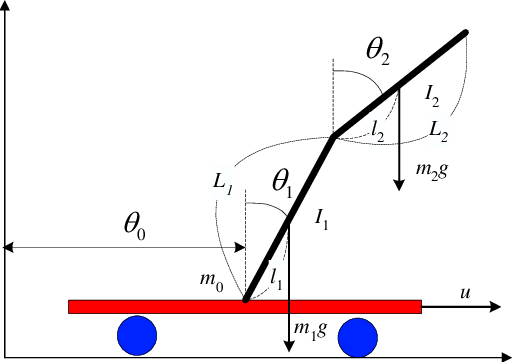
\includegraphics[width=0.4\textwidth]{figures/Double-inverted-pendulum-on-a-cart.png} % Replace "example-image" with the actual image file name and path
  \caption{Double inverted pendulum on a cart\cite{bogdanov2004optimal}}
  \label{fig:DIPC}
\end{figure}

Another significant variation is the Furuta pendulum\cite{cazzolato2011dynamics}, initially developed at the Tokyo Institute of Technology by Furuta and his colleagues\cite{furuta1992swing}. This system comprises a driven arm that rotates horizontally and a pendulum attached to this arm, allowing free vertical rotation. Due to the influence of gravitational forces and the coupling stemming from Coriolis and centripetal forces, the Furuta pendulum is characterized by its underactuation and highly nonlinear behavior.

\begin{figure}[H]
  \centering
  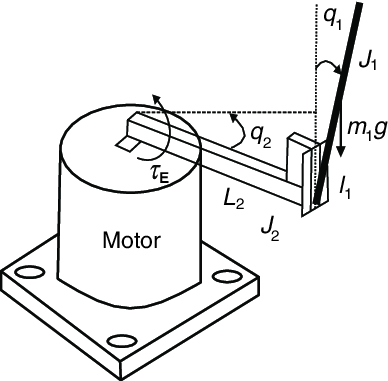
\includegraphics[width=0.4\textwidth]{figures/Furuta-pendulum.png} % Replace "example-image" with the actual image file name and path
  \caption{Furuta pendulum\cite{aguilar2010direct}}
  \label{fig:Furuta pendulum}
\end{figure}

The double pendulum utilized in this thesis represents a third variation. It consists of two links connected in series by revolute joints. Unlike the Furuta pendulum, both links of the double pendulum move in the same plane within three-dimensional space. These two links are connected to the world frame via revolute joints as well. In contrast to the DIPC setup, the actuation capability is solely limited by the torque that the joints can generate, unrestricted by the length of a prismatic rail. The dynamics of the double pendulum system will be discussed in the following section.

\subsection{Dynamics of underactuated double pendulum system}
As shown in Figure \ref{fig:double pendulum dynamics}, we model the dynamics of the double pendulum with 15 parameters which include 8 link parameters namely masses \((m_1,m_2)\)
, lengths \((l_1,l_2)\)
, center of masses \((r_1,r_2)\) 
, inertias \((I_1,I_2)\)
 for the two links, and 6 actuator parameters namely motor inertia \(I_r\)
, gear ratio \(g_r\)
, coulomb friction \((c_{f1},c_{f2})\)
, viscous friction \((b_1,b_2)\)
 for the two joints and gravity.
\begin{figure}[h]
  \centering
  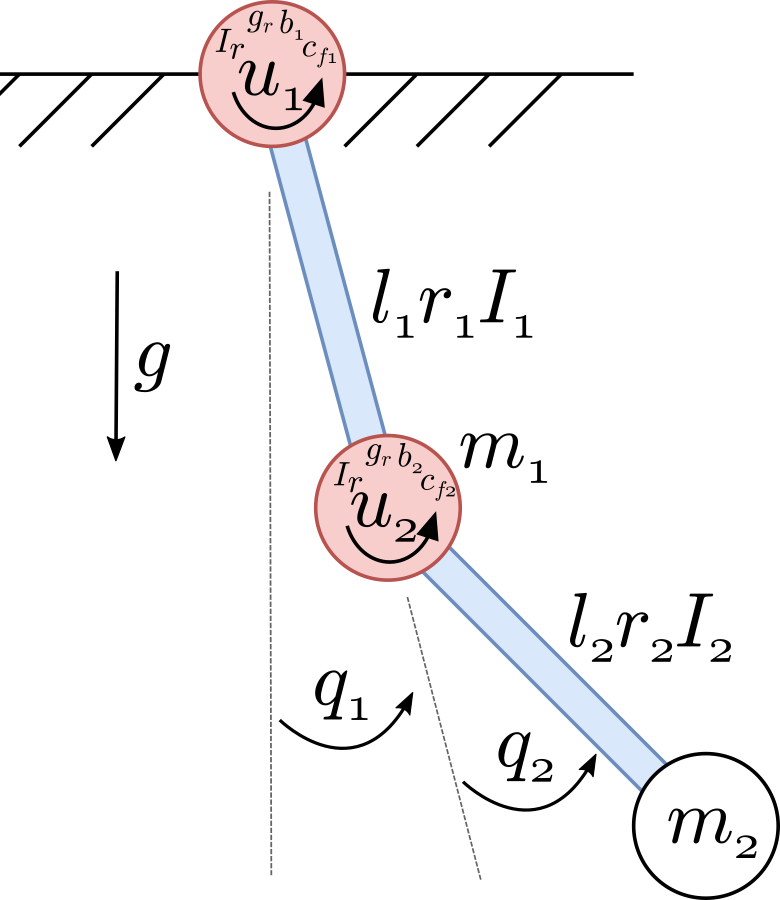
\includegraphics[width=0.5\textwidth]{figures/double_pendulum_dynamics.png} % Replace "example-image" with the actual image file name and path
  \caption{Double pendulum dynamics}
  \label{fig:double pendulum dynamics}
\end{figure}

The generalized coordinates \( \mathbf{q} =[q_1,q_2]^T \) are the joint angles measured from the free hanging position. The state vector of the systems contains the position coordinates and their time derivatives: \(\mathbf{x}=[\mathbf{q},\mathbf{\dot{q}}]^T\). The torque applied by the actuators are \(\mathbf{u}=[u_1,u_2]\). The equation of motion for the dynamics of a dynamical system can be derived following the blow steps:

\textbf{Step 1. Define the Lagrangian (\(L\)):}

   The Lagrangian (\(L\)) is defined as the difference between the kinetic energy (\(T\)) and the potential energy (\(U\)) of the system:
   \begin{align}
         L = T - U
   \end{align}


\textbf{Step 2. Express the Kinetic Energy (\(T\)):}

   The kinetic energy (\(T\)) of the double pendulum is the sum of the kinetic energies of both links. The kinetic energy for a link is given by:
   \begin{align}
        \label{eq:kinetic energy}
        T = \frac{1}{2} m_1 (\dot{x}_1^2 + \dot{y}_1^2) + \frac{1}{2} m_2 (\dot{x}_2^2 + \dot{y}_2^2)
   \end{align}

   where \(m_1\) and \(m_2\) are the masses of the links, \((x_1, y_1)\) and \((x_2, y_2)\) are their positions, and \(\dot{x}_1, \dot{y}_1, \dot{x}_2, \dot{y}_2\) are their respective velocities.

\textbf{Step 3. Express the Potential Energy (\(U\)):}

   The potential energy (\(U\)) of the double pendulum is the sum of the potential energies of both links. The potential energy for a link in a gravitational field is given by:
   \begin{align}
         \label{eq:potential energy}
         U = m_1 g y_1 + m_2 g y_2
   \end{align}

   where \(g\) is the acceleration due to gravity.
   
   
\textbf{Step 4. Formulate the Lagrange's Equation:}

   Use Lagrange's equation to derive the equations of motion for the generalized coordinates \(x_1, y_1, x_2, y_2\).

    \begin{align}
    \label{eq:lagrange equation}
    \frac{d}{dt} \left(\frac{\partial L}{\partial \dot{q_i}}\right) - \frac{\partial L}{\partial q_i} = 0
    \end{align}

\textbf{Step 5. Solve the Equations of Motion:}

   Solve the obtained set of second-order differential equations to determine the equations of motion for the system. The system dynamics with friction is:
   
   \begin{align}
        \label{eq:EoM}
        M(q)\ddot{q} + C(q,\dot{q})\dot{q} &= Du + G(q) - F(\dot{q})
   \end{align}
    
    Because the state vector is \(\mathbf{x}=[\mathbf{q},\mathbf{\dot{q}}]^T\), the equation of motion can also be expressed as:
    
    \begin{equation}
    \begin{split}
        \dot{x} &= f(x,u) \\
        &= \begin{bmatrix} 
            \dot{q} \\ 
            M^{-1}(Du - C(q,\dot{q})\dot{q} + G(q) - F(\dot{q})) 
       \end{bmatrix}
    \end{split}
    \end{equation}

   Consider the forward kinematics of double pendulum system, the coordinate of the joint between the first link and the second link is \(P_1=(x_1,y_1)\),the coordinate of the end effector is \(P_2=(x_2,y_2)\).

    \begin{align}
        \label{eq:p1}
        \left\{
        \begin{aligned}
        x_1 &= l_1 \sin(q_1) \\
        y_1 &= - l_1 \cos(q_1)
        \end{aligned}
        \right.
    \end{align}

    \begin{align}
        \label{eq:p2}
        \left\{
        \begin{aligned}
        x_2 &= l_1 \sin(q_1) + l_2 \sin(q_1 + q_2) \\
        y_2 &= -l_1 \cos(q_1) - l_2 \cos(q_1 + q_2)
        \end{aligned}
        \right.
    \end{align}

    Put Equation \ref{eq:p1} and \ref{eq:p2} into \ref{eq:kinetic energy}, \ref{eq:potential energy}, \ref{eq:lagrange equation}, \ref{eq:EoM},we can get the mass matrix (with \(s_1 = \sin(q_1), c_1 = \cos(q_1), \ldots\))
    \begin{equation}
    \mathbf{M} =
    \left[ 
    {\begin{array}{cc}
    I_1 + I_2 + l_1^2m_2 + 2l_1m_2r_2c_2 + g_r^2I_r + I_r  &   I_2 + l_1m_2r_2c_2 - g_rI_r  \\
    I_2 + l_1m_2r_2c_2 - g_rI_r                    & I_2 + g_r^2I_r                       \\
    \end{array}} 
    \right]
    \end{equation}
    
    The Coriolis matrix:
    
    \begin{equation}
    \begin{split}
    \mathbf{C} = \left[
    \begin{matrix}
    -2 \dot{q}_2 l_{1} m_{2} r_{2} \sin(q_2) & -\dot{q}_2 l_{1} m_{2} r_{2} \sin(q_2)\\
    \dot{q}_1 l_{1} m_{2} r_{2} \sin(q_2) & 0
    \end{matrix}
    \right],
    \label{eq:coriolis_matrix}
    \end{split}
    \end{equation}
    
    The gravity vector:
    
    \begin{equation}
    \begin{split}
    \mathbf{G} = \left[
    \begin{matrix}
    - g m_{1} r_{1} \sin(q_1) - g m_{2} \left(l_{1} \sin(q_1) + r_{2} \sin(q_{1+2}) \right) \\
    - g m_{2} r_{2} \sin(q_{1+2})
    \end{matrix}
    \right],
    \label{eq:gravity_matrix}
    \end{split}
    \end{equation}
    
    The friction vector:
    
    \begin{equation}
        \begin{split}
            \mathbf{F} =
            \left[
                \begin{matrix}
                    b_1 \dot{q}_1 + c_{f1} \arctan(100\,\dot{q}_1) \\
                    b_2 \dot{q}_2 + c_{f2} \arctan(100\,\dot{q}_2)
                \end{matrix}
            \right]
        \end{split}
    \end{equation}
    (the \(\arctan(100\,\dot{q}_i)\) function is used to approximate the discrete step function for the coulomb friction)

    And the actuator selection matrix \(\mathbf{D}\):
    
    \begin{equation}
        \begin{split}
            \mathbf{D}_{full} =
            \left[
                \begin{matrix}
                    1 & 0 \\
                    0 & 1
                \end{matrix}
            \right],
            \quad
            \mathbf{D}_{pendu} =
            \left[
                \begin{matrix}
                    1 & 0 \\
                    0 & 0
                \end{matrix}
            \right],
            \quad
            \mathbf{D}_{acro} =
            \left[
                \begin{matrix}
                    0 & 0 \\
                    0 & 1
                \end{matrix}
            \right]
        \end{split}
    \end{equation}
    
    for the fully actuated system, the pendubot or the acrobot.

\section{Related work}
This thesis focuses on learning-based robotic motion control, a field that has garnered increasing attention in recent years, with significant contributions from various research institutes.

Today, much of the research in this field is conducted within simulation environments due to their cost-effectiveness and the ability to facilitate rapid iteration. One noteworthy project from 2018 is the DeepMimic project\cite{peng2018deepmimic}, undertaken by researchers at the University of California, Berkeley. This work resides at the intersection of deep reinforcement learning, imitation learning, and robotics.

The DeepMimic project utilizes physics-based simulations to successfully replicate the diverse range of behaviors exhibited in the real world by 3D characters. These characters include real-world examples such as humanoid and Atlas robotics, as well as fictional characters like T-Rexes and dragons. Instead of relying on manually designed controllers, the project employs deep reinforcement learning methods to generalize to new skills and situations, often without human intervention.

In the training process, the agent is provided with reference data recorded by motion capture actors or keyframed animations. Through imitation learning, the agent is guided to achieve specific predefined goals. The central contribution of this project lies in its framework, which combines goal-directed reinforcement learning with reference data generated by humans. This combination enables the imitation of a wide variety of motion skills.

\begin{figure}[H]
  \centering
  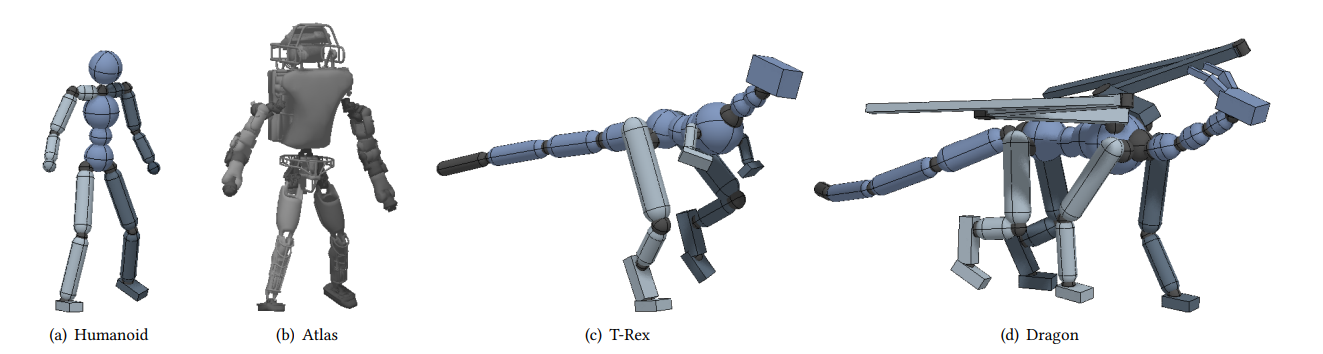
\includegraphics[width=1.1\textwidth]{figures/deepmimic.png} % Replace "example-image" with the actual image file name and path
  \caption{3D characters in Deepmimic project\cite{peng2018deepmimic}}
  \label{fig:deepmimic}
\end{figure}

In the context of reinforcement learning, a distinction exists between model-free and model-based approaches. Model-free reinforcement learning(MFRL) does not require information about the transition model, whereas model-based reinforcement learning(MBRL) leverages the transition model to make decisions based on a prior known model or one learned from interactions.

The model-free approach is notably characterized by its sample inefficiency. Successful training often takes many hours, if not days or weeks.

An intriguing project that relies solely on model-free deep reinforcement learning is the Learning-to-Walk-in-20 Minutes project\cite{smith2022walk} conducted by researchers from UC Berkeley. They employ an algorithmic framework closely related to DroQ \cite{hiraoka2021dropout}, an extension of the SAC algorithm \cite{haarnoja2018soft} incorporating dropout \cite{srivastava2014dropout} and layer normalization \cite{ba2016layer}. Remarkably, their training is conducted directly on the real system. They demonstrate that current deep RL methods can effectively teach quadrupedal locomotion in under 20 minutes, a stark contrast to previous research conducted by Kumar et al. \cite{kumar2021rma}, which employed the same hardware but required \(1.2 \times 10^9\) samples to train a robust controller for locomotion. This corresponds to roughly 4.5 months' worth of cumulative experience.

Model-based reinforcement learning is recognized for its integration of an environment model with trial-and-error learning. One notable advantage is the potential for higher sample efficiency compared to the model-free approach. This work, conducted by the University of Toronto\cite{wang2019benchmarking}, provides a comprehensive comparison by benchmarking model-based reinforcement learning.

\begin{figure}[H]
  \centering
  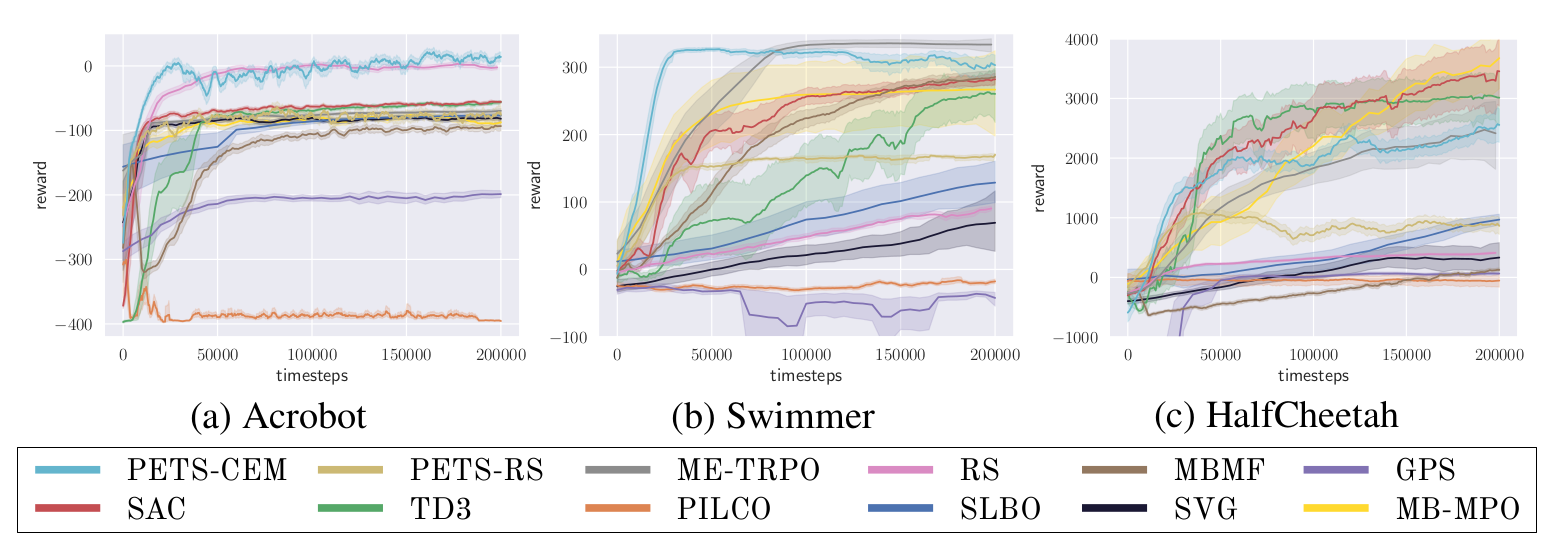
\includegraphics[width=0.9\textwidth]{figures/benchmarking_mbrl.png} % Replace "example-image" with the actual image file name and path
  \caption{Benchmarking model-based reinforcement learning\cite{wang2019benchmarking}}
  \label{fig:benchmarking MBRL}
\end{figure}

The team has collected 11 Model-Based Reinforcement Learning (MBRL) algorithms and 4 Model-Free Reinforcement Learning (MFRL) algorithms across 18 benchmarking environments specifically designed for MBRL in simulation. These benchmarking environments are based on the standard OpenAI Gym\cite{brockman2016openai}, ranging from simple 2D tasks like cart-pole to complex setups like humanoid. The benchmarking process is further extended by introducing noise into the environment, including disturbances in observations and actions.

The team has discovered that while 1 million time-step training is common for MFRL algorithms, many MBRL algorithms converge much earlier, often within 200k time-steps. Within the field of MBRL, when it comes to the evaluation of sample efficiency, asymptotic performance, and robustness, there is no clear and consistent best MBRL algorithm. This leaves ample opportunities for future research to leverage the strengths of different approaches.

Another notable challenge in reinforcement learning-based robotic control is the sim-to-real gap problem. Since agents are typically trained in carefully designed simulated worlds, these simulations can sometimes be idealized or oversimplified to some extent. Consequently, the optimal policy derived from the simulation often fails to account for the uncertainties of the real world, leading to failures when executing intended tasks. There are several approaches to bridging the sim-to-real gap, and the following work presents an interesting approach.

A research team from ETH Zurich has made significant progress in addressing the sim-to-real interface challenge \cite{hwangbo2019learning}. Their methodology involves training a control model for a quadruped robot within a simulation environment. By utilizing a neural network and leveraging data collected from the real robot, they approximated the dynamics model of the physical robot. This approach has facilitated the accurate implementation of the control policy derived from the virtual environment onto the real robot. These exemplary works demonstrate the promising applications of learning-based approaches in various aspects of robot control.

\begin{figure}[H]
  \centering
  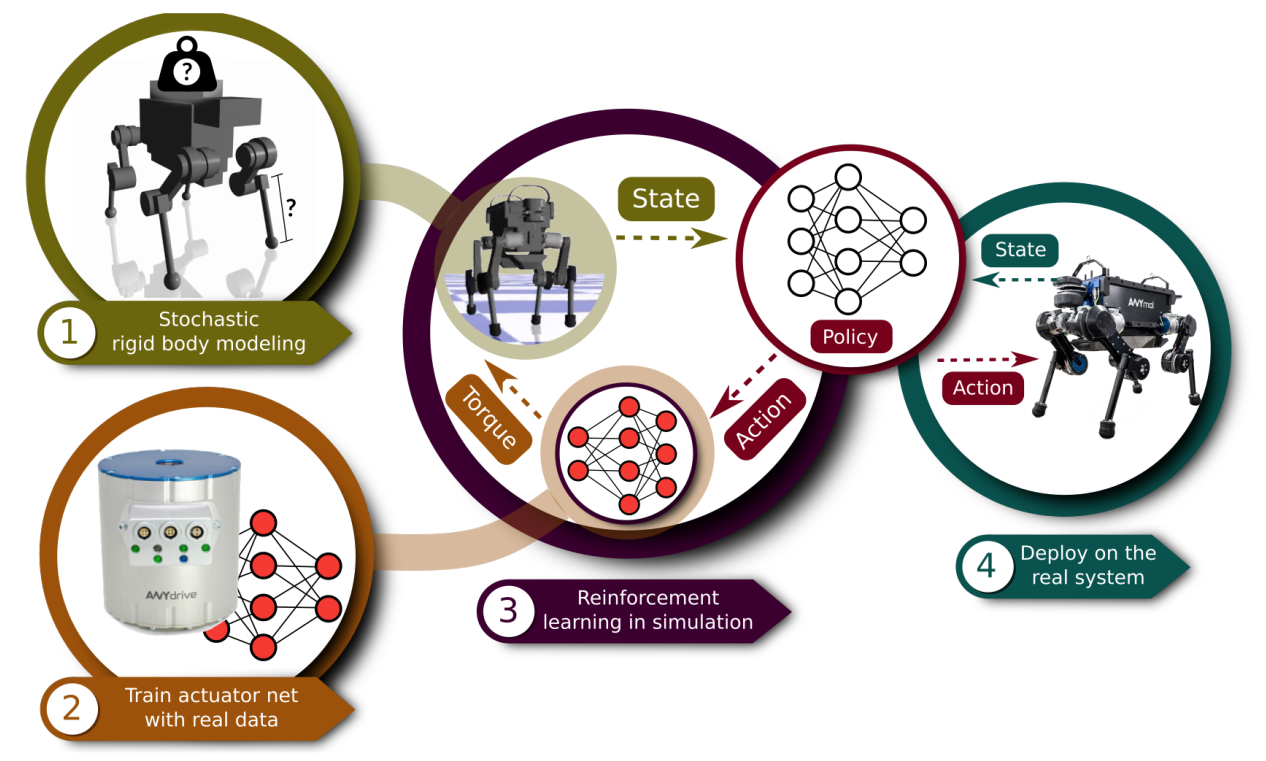
\includegraphics[width=0.9\textwidth]{figures/quadruped_sim2real.png} % Replace "example-image" with the actual image file name and path
  \caption{Sim-to-real framework for RL-based quadruped controller\cite{hwangbo2019learning}}
  \label{fig:benchmarking MBRL}
\end{figure}

In conclusion, in the field of reinforcement learning-based control in robotics, researchers currently face three major challenges:

\begin{enumerate}
    \item \textbf{Sample Inefficiency in Model-Free Reinforcement Learning:}
    
    Model-free reinforcement learning is known for its sample inefficiency, where the time required for random trial and error can be excessively long.
    
    \item \textbf{Immaturity of Model-based RL} 
    
    Model-based reinforcement learning is a growing force but still in its infancy. Finding the right balance between model information and reinforcement learning remains an ongoing challenge.
    
    \item \textbf{Sim-to-Real Gap Limitations:} 
    
    Deploying controllers learned through reinforcement learning on real systems is limited due to the significant sim-to-real gap. This limitation confines a substantial portion of research to simulations.
\end{enumerate}

The research community has much work to do before reinforcement learning becomes a stable and widely accepted approach in the industry.


\cleardoublepage

\chapter{Methodology}
The primary goal of this thesis is to achieve the swing-up movement in the pendubot or acrobot setup and to maintain stability around the highest points. Challenges have been revealed in initial training trials with reinforcement learning, including potential entrapment in local minima and difficulty in maintaining stability at the highest point for extended periods.

To address these challenges, two main strategies are adopted. For the stabilization issue, a combined controller is introduced. During the swing-up process, control is assumed by an RL-trained agent, utilizing the Soft Actor-Critic—a classic model-free reinforcement learning algorithm—based on its learned policies. However, as the system nears the maximum point, a seamless transition occurs. This shift allows for the takeover of control by a continuous-time LQR controller, ensuring the final stabilization required to maintain stability at the highest point. For the entrapment in local minima problem, a carefully designed reward function is utilized to guide the agent away from hazadous local minima and achieve successful swing up.

\section{Soft actor critic}
Within the landscape of reinforcement learning, the Soft Actor Critic (SAC)\cite{haarnoja2018soft} stands out as an algorithm specifically designed for environments with continuous state and action spaces. Such environments, exemplified by our double pendulum system where actuators can be adjusted to any value within the torque limit range, and state measurement can take any real number, influenced our decision to adopt SAC.

Like many other deep reinforcement learning algorithms, SAC optimizes a policy by maximizing the expected cumulative reward the agent obtains over time. This optimization is primarily achieved through an actor-critic structure\cite{konda1999actor}.

The actor determines the best actions by interpreting the current environmental conditions and adhering to the existing policy. Typically, the actor is visualized as a shallow neural network that approximates the mapping between the input state and the output probability distribution over actions. Furthermore, SAC incorporates a stochastic policy within its actor, which fosters exploration and aids the agent in refining its policies.

On the other hand, the critic evaluates the value of state-action pairs. It estimates the expected cumulative reward the agent can achieve by following a particular policy. More often than not, the critic is depicted as a neural network that processes state-action pairs as inputs to yield the estimated value.

A distinguishing feature of SAC, besides the actor-critic framework, is entropy regularization\cite{achiam2018spinning}. SAC utilizes a stochastic policy. This means that instead of always settling on a single best action for each state, the agent considers a probability distribution over potential actions. The incorporation of entropy in SAC aims to encourage exploration: high entropy signifies a more uniform distribution, implying the agent's uncertainty and tendency to explore diverse actions, while low entropy points to a concentrated distribution, suggesting the agent's confidence in a specific action. By definition, entropy quantifies randomness. Within SAC, it captures the unpredictability of the policy's action distribution. If
\(x\) is a random variable with a probability density function \(P\), the
entropy \(H\) of \(x\) is defined as:

\begin{equation}
 H(P) = \displaystyle \mathop{\mathbb{E}}_{x \sim P}[-\log P(x)]
\end{equation}

By maximizing entropy, SAC encourages exploration and accelerates learning. It
also prevents the policy from prematurely converging to a suboptimal solution.
The trade-off between maximizing reward and maximizing entropy is controlled
through a parameter, \(\alpha\). This parameter serves to balance the importance
of exploration and exploitation within the optimization problem. Each interactioin between the agent and the environment can be recorded as a tuple \((s_t,a_t,R,s_{t+1})\). The optimal policy
\(\pi^*\) can be defined as follows:

\begin{equation}
 \pi^* = {arg}{\max_{\pi}}{\displaystyle
 \mathop{\mathbb{E}}_{\tau\sim\pi}}{\Bigg[{\sum_{t=0}^{\infty}}{\gamma^{t}}{\Big(R(s_t,a_t,s_{t+1})}+{\alpha}H(\pi(\cdot\mid{s_t}))\Big)\Bigg]}
\end{equation}

Where \(s_t\) and \(a_t\) represent the state and action at time \(t\), and \(s_{t+1}\) represents the state at time \(t+1\). \(R\) denotes the immediate reward received by the agent after taking action \(a_t\) in state \(s_t\), while \(\gamma\) is the discount factor that determines the agent's emphasis on long-term cumulative rewards over immediate ones.

During training, SAC learns a policy $\pi_{\theta}$ and two Q-functions
$Q_{\phi_1} , Q_{\phi_2}$ concurrently. The loss functions for the two Q-networks are
$(i \in {1, 2})$:

\begin{equation}
  L(\phi_i,D) = \displaystyle
  \mathop{\mathbb{E}}_{(s,a,r,s',d)\sim{D}}\bigg[\bigg(Q_{\phi_i}(s,a)-y(r,s',d)\bigg)^2\bigg],
\end{equation}

where the temporal difference target \(y\) is given by:

\begin{align}
  y(r,s',d) &= r + \gamma(1-d) \times \nonumber\bigg(\displaystyle
  \mathop{\min}_{j=1,2}Q_{\phi_{targ,j}}(s',\tilde{a}')-\alpha\log
  {\pi_\theta}(\tilde{a}'\mid{s}')\bigg), \\
  \tilde{a}'&\sim{\pi_\theta}(\cdot\mid{s'})
\end{align}

In each state, the policy \(\pi_\theta\) should act to maximize the expected
future return \(Q\) while also considering the expected future entropy \(H\). In other
words, it should maximize \(V^\pi(s)\):

\begin{align}
 V^\pi(s) &= {\displaystyle \mathop{\mathbb{E}}_{a\sim\pi}[Q^\pi(s,a)]} +
 \alpha{H(\pi(\cdot\mid{s}))} \\
 &= {\displaystyle \mathop{\mathbb{E}}_{a\sim\pi}[Q^\pi(s,a)} -
 \alpha{\log {\pi(a\mid{s})]}}
\end{align}

The interaction experiences are stored as tuples \((s, a, r, s', d)\) in a replay buffer \(\textit{D}\). Here, \(d\) represents the signal for episode termination. When it is time to update the Q-value and policy, a batch of transitions \(\textit{B} = \{(s, a, r, s', d)\}\) is randomly sampled from \(\textit{D}\). The Q-functions are updated by one step of gradient descent, the gradients of the loss functions for the Q-networks are calculated by:

\begin{equation}
\nabla_{\phi_i} \frac{1}{|\textit{B}|} \sum_{(s, a, r, s', d) \in \textit{B}} \left(Q_{\phi_i}(s, a) - y(r, s', d)\right)^2 \quad \text{for} \quad i=1,2
\end{equation}

The policy is updated using one step of gradient ascent, the gradient is expressed as:

\begin{equation}
\nabla_{\theta} \frac{1}{|\textit{B}|} \sum_{s \in \textit{B}}\left(\min\limits_{\substack{i=1,2}}Q_{\phi_i}(s,\widetilde{a}_{\theta}(s)) - \alpha \log\pi_{\theta}(\widetilde{a}_{\theta}(s)|s)\right)
\end{equation}

where \(\widetilde{a}_{\theta}(s)\) is a sample of action derived from \(\pi_\theta(\cdot|s)\) which is differentiable with respect to \(\theta\). 

In conclusion, SAC's combination of stochastic policies, exploration through
entropy regularization, value estimation, and gradient-based optimization make
it a well-suited algorithm for addressing the challenges posed by continuous
state and action spaces.

\section{Linear quadratic regulator}
The Linear Quadratic Regulator (LQR)\cite{lehtomaki1981robustness} is an effective control method primarily designed for linear systems. Yet, when dealing with nonlinear dynamics, it remains applicable. The nonlinear system is linearized around a selected operating point, and based on this linearized version, the LQR controller can be sculpted.

Taking a step back, the general form of a nonlinear system defined by state vector \(x\) and input vector \(u\) can be expressed as:
\begin{equation}
 \dot{x}(t) = f(x(t), u(t))
\end{equation}

In certain applications, such as pendubot or acrobot stabilization, it is important to select the appropriate operating point. Due to the tasks to be completed, the operating point is chosen around the upright position, specifically \(x_{op} = [\pi,0,0,0]^T\). Around this point, the system can be linearized, leading to:

\begin{equation}
\dot{\overline{x}}(t) = A \overline{x}(t) + B u(t)
\end{equation}

Here, the deviation from the desired state is given by \(\overline{x} = x - x_{\text{op}}\). Its first derivative, \(\dot{\overline{x}} = \dot{x} - \dot{x}_{\text{op}} = \dot{x}\), for \(x_{\text{op}}\) being a constant. The linearized state matrices \(A\) and input matrix \(B\) around the operation point are derived as:

\begin{equation}
A = \left.\frac{\partial f}{\partial x}\right|_{x = x_{\text{op}}}, \quad B = \left.\frac{\partial f}{\partial u}\right|_{x = x_{\text{op}}}
\end{equation}

To derive an optimal control strategy, a quadratic cost function \(J\) is needed:

\begin{equation}
  J = \int_0^{T} \left( x^T Q x + u^T R u \right) \, dt
  \label{eq:quadratic_cost}
\end{equation}

The matrices \(Q\) and \(R\) must be chosen to be symmetric and positive definite, which means \(Q = Q^T\) with all its eigenvalues positive, and similarly, \(R = R^T\) with all positive eigenvalues.

The Hamilton-Jacobi-Bellman equation (HJB) characterizes the optimal value function \(J^*(x)\), representing the minimum cost-to-go from state \(x\) to termination at \(T\). The HJB equation is as follows:

\begin{equation}
 \frac{dJ^*(x)}{dt} = \min_u \left( x^T Q x + u^T R u + \frac{dJ^*(x)}{dx} (Ax + Bu) \right)
 \label{eq:HJB}
\end{equation}

By calculating \(\frac{dJ^*(x)}{dt}\) from Equation \ref{eq:quadratic_cost}, the HJB equation can be reduced to the continuous-time algebraic Riccati equation:

\begin{equation}
 A^T S + SA - SBR^{-1}B^T S + Q = 0
\end{equation}

Finally, the LQR control law obtained with the above method for this linearized system is:

\begin{equation}
 u(t) = -K\overline{x}(t)
\end{equation}

where \(K = R^{-1}B^T S\).

For a LQR controller like this, torques will always be applied to steer the system state toward the origin of the linear system.


\section{Combining SAC and LQR with region of attraction}
In our approach, a combined control method is utilized for both the swing-up and stabilization tasks. This combined control framework is a natural choice and has previous work that supports this method. In this work by S. Gillen et al.\cite{gillen2020combining}, a similar structure combining a local controller and a learned controller with a gate function was employed. The work was conducted on chaotic control of an acrobot setup in simulation, which resembles our project.

In our implementation, during the swing-up phase, the SAC controller is employed. Once the state of the double pendulum approaches the vicinity of the desired goal state, the transition from the SAC controller to the LQR controller is made for final-stage stabilization. An essential aspect of any combined control strategy is the determination of the conditions under which the system is ready for a transition between control methods. In our SAC+LQR control strategy, the gate function for making this determination is provided by the region of attraction method\cite{maywald2022co}.

\begin{figure}[H]
    \centering
    
\includegraphics[width=0.8\textwidth]{figures/methodology/combined_controller.png}
    \caption{Combined controller}
    \label{fig:combined_controller}
\end{figure}

The region of attraction (RoA) for a nonlinear system, denoted as \(R_a\), describes the set of initial states surrounding a fixed point \(x_0\). If a state lies within this region, the system will converge towards \(x_0\) as \(t \rightarrow \infty\). In the context of an LQR controller, the RoA signifies the area within the state space where the controlled system exhibits asymptotic stability. For complex systems, directly computing \(R_a\) can be challenging; instead, it is often estimated. The simplest way to estimate such a set requires the assistance of a Lyapunov function \(V(x)\) bounded by a scalar \(\rho\)\cite{khalil2002nonlinear}.

\begin{equation}
 B = \{x|V(x)<\rho\}
\end{equation}

Here, \(B\) represents the estimated subset of the real region of attraction \(R_a\). 

The goal is to find the largest \(\rho\) for which the Lyapunov conditions are satisfied. These conditions are as follows:

\begin{equation}
\begin{cases}
   V(x) > 0 \\
   \dot{V}(x) < 0 & \text{for} \quad x \in B
\end{cases}
\label{eq:V_conditions}
\end{equation}

The Lyapunov function for a controlled linear system, \(\dot{x}(t) = (A - BK)x(t)\), is chosen in a quadratic form:

\begin{equation}
  V(x) = x^T S_{LQR} x 
  \label{eq:V}
\end{equation}

Here \(S_{LQR}\) is a positive definite matrix. This function serves as an 'energy-like' metric. Next, we calculate the time derivative of the Lyapunov function.For the infinite horizon LQR, \(\frac{\partial S_{LQR}}{\partial t} = 0\) and \(\frac{\partial x_0}{\partial t} = 0\), hence, \(\dot{V}\) is:

\begin{equation}
\dot{V}(x) = 2x^{T}S_{LQR}\dot{x}
\label{eq:V_dot}
\end{equation}

Combining equations and conditions \ref{eq:V_conditions}, \ref{eq:V}, \ref{eq:V_dot}, we have the following expression:

\begin{equation}
\begin{cases}
    B = \{ x \mid 0 < V(x) < \rho \} \\
    \dot{V}(x) = 2x^T S_{LQR} \dot{x} < 0
\end{cases}
\end{equation}

The RoA is computed similar to \cite{maywald2022co} but with a sums of squares method\cite{tedrake2010lqr}. The resulting shape of the RoA in a 4D state space resembles an ellipsoid.

\begin{figure}[H]
    \centering
    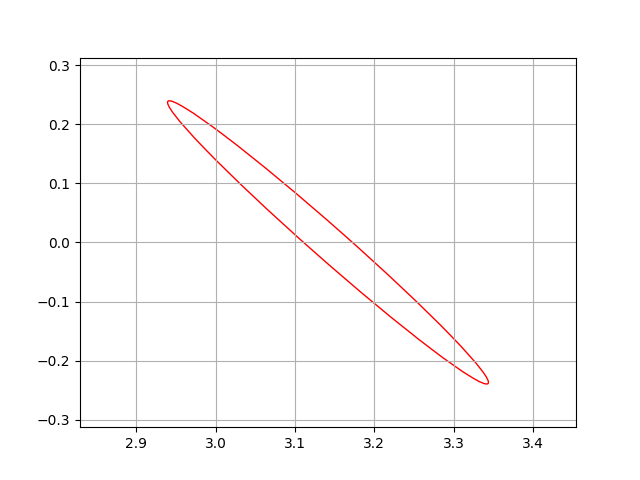
\includegraphics[width=0.6\textwidth]{figures/methodology/roaplot.png} % Adjust the width as needed
    \caption{Region of Attraction[redraw this figure]}
    \label{fig:example}
\end{figure}

Once the RoA is computed, it can be checked whether a state \(x\) belongs to the estimated RoA of the LQR controller by calculating the cost-to-go of the LQR controller with the matrix \(S_{LQR}\) and comparing it with the scalar \(\rho\).

\section{Reward shaping}
The reward function is intended to guide the agent in performing desired behavior. In our design, the reward function aims to guide the double pendulum system towards achieving stability around the highest point.

One of the primary reasons why controlling an underactuated double pendulum system using RL is so challenging is the state space that can lead to successful stabilization is very small. Initial training attempts using OpenAI Gym Acrobot-v1\cite{towers_gymnasium_2023} rewards have revealed this challenge. For instance, the agent may accidentally get close to the goal state but not receive enough reward. This can result in being stuck in an unsuitable position for an extended period or a high-speed rotation of the second link with the first link almost upright. 

Another significant challenge in our RL-based training is that, due to our plan for real hardware deployment, the dynamic model of the double pendulum is more detailed than that of most simulation environments like OpenAI Gym Acrobot-v1\cite{towers_gymnasium_2023}. Because we are using quasi-direct drive motors to simplify joint dynamics, one of the significant drawbacks of this motor type is its low gear ratio, resulting in a relatively low torque limit (5 Nm).

Therefore, there is a need for an innovative reward function design suitable for our problem setup. To tackle the swing-up issue, a customized three-stage reward function is designed to steer the agent away from problematic local minima and into the region of attraction of the LQR controller. The full equation for this reward function is:

\begin{equation}
\begin{aligned}
 r(x,u) = &-(x - x_g)^T Q_{train} (x - x_g) - u^T R_{train}u \\
           & +
            \begin{dcases*}
              r_{line} & \text{if} $h(p_1, p_2) \geq h_{line}$\, ,\\
              0 & \text{else}
            \end{dcases*}\\
           & +
            \begin{dcases*}
              r_{LQR} & \text{if} $(x - x_g)^T S_{LQR} (x - x_g) \geq \rho $\, ,\\
              0 & \text{else}
            \end{dcases*}\\
           & -
            \begin{dcases*}
              r_{vel} & \text{if} $|v_1| \geq v_{thresh}$\, ,\\
              0 & \text{else}
            \end{dcases*}\\
           & -
            \begin{dcases*}
              r_{vel} & \text{if} $|v_2| \geq v_{thresh}$\, ,\\
              0 & \text{else}
            \end{dcases*}
\end{aligned}
\end{equation}

In the initial stage, a quadratic reward function is employed to encourage
smooth swinging of the entire system within a relatively small number of
training sessions. The matrix  \(Q_{train} = diag(Q_1, Q_2, Q_3, Q_4)\) is a
diagonal matrix, while \(R_{train}\) is a scalar. This is due to the nature
of underactuated control in the double pendulum system, where only a single
control input is available.

\begin{figure}[H]
    \centering
    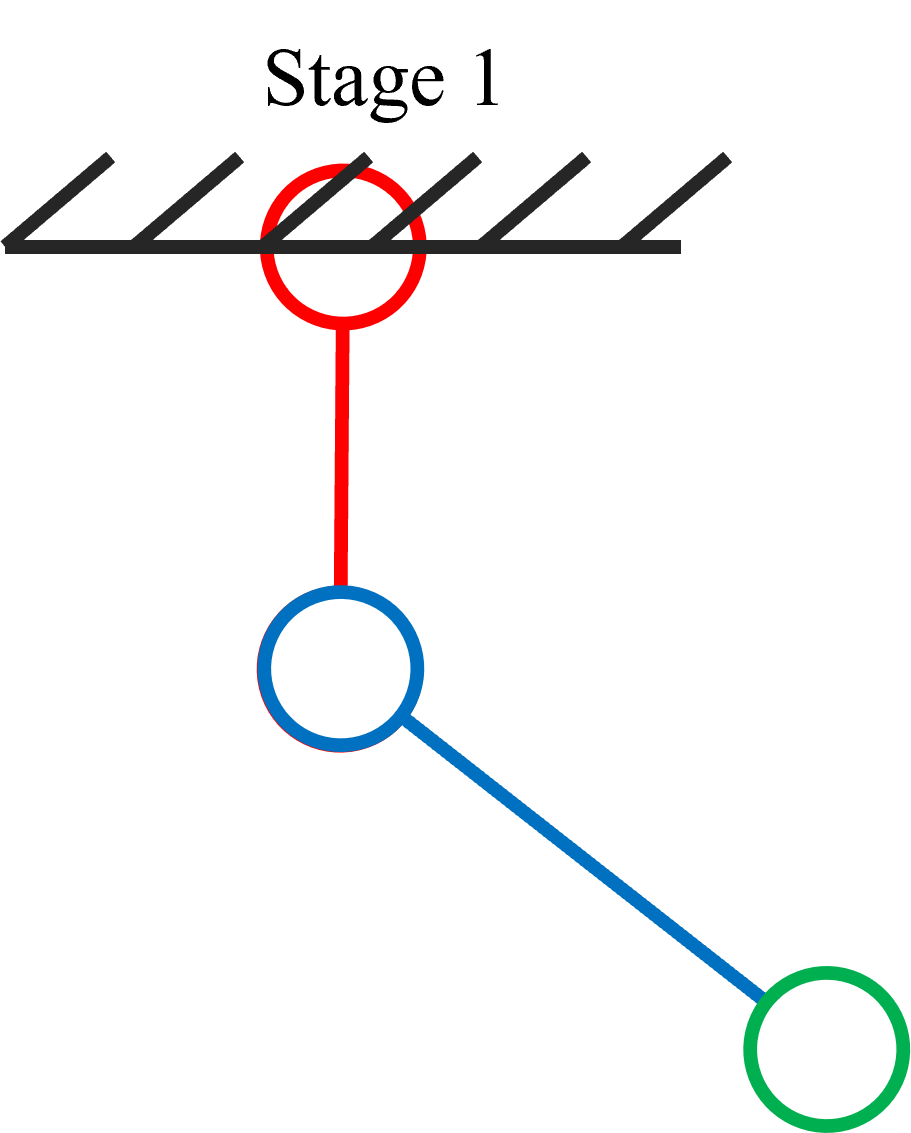
\includegraphics[width=0.25\textwidth]{figures/methodology/stage1.png} % Adjust the width as desired
    \caption{Swing up stage 1}
    \label{fig:stage1} % Optional label for referencing
\end{figure}

As the end effector reaches a threshold line \(h_{line} = 0.8(l_1+l_2)\), we
introduce a second level of reward \(r_{line}\). The end effector height is
given by
\begin{align}
    h(p_1, p_2) = -l_1\cos(p_1) - l_2 \cos(p_1 + p_2).
\end{align}

with the link lengths $l_1$ and $l_2$.
This reward provides the agent with a fixed value
but is carefully designed to prevent the system from spinning rapidly in either
clockwise or counterclockwise directions. To discourage the agent from
exploiting rewards by spinning at excessive speeds, a significant penalty
\(-r_{vel}\) is implemented for any speed exceeding $v_{thresh}=8\,
\text{rad}/\text{s}$ in absolute value.
This penalty effectively compels the agent to approach the maximum point while
adhering to the predefined speed interval(less than 20 rad/s). The speed penalty was only needed for the acrobot when the experiments are confined in simulation.

\begin{figure}[H]
    \centering
    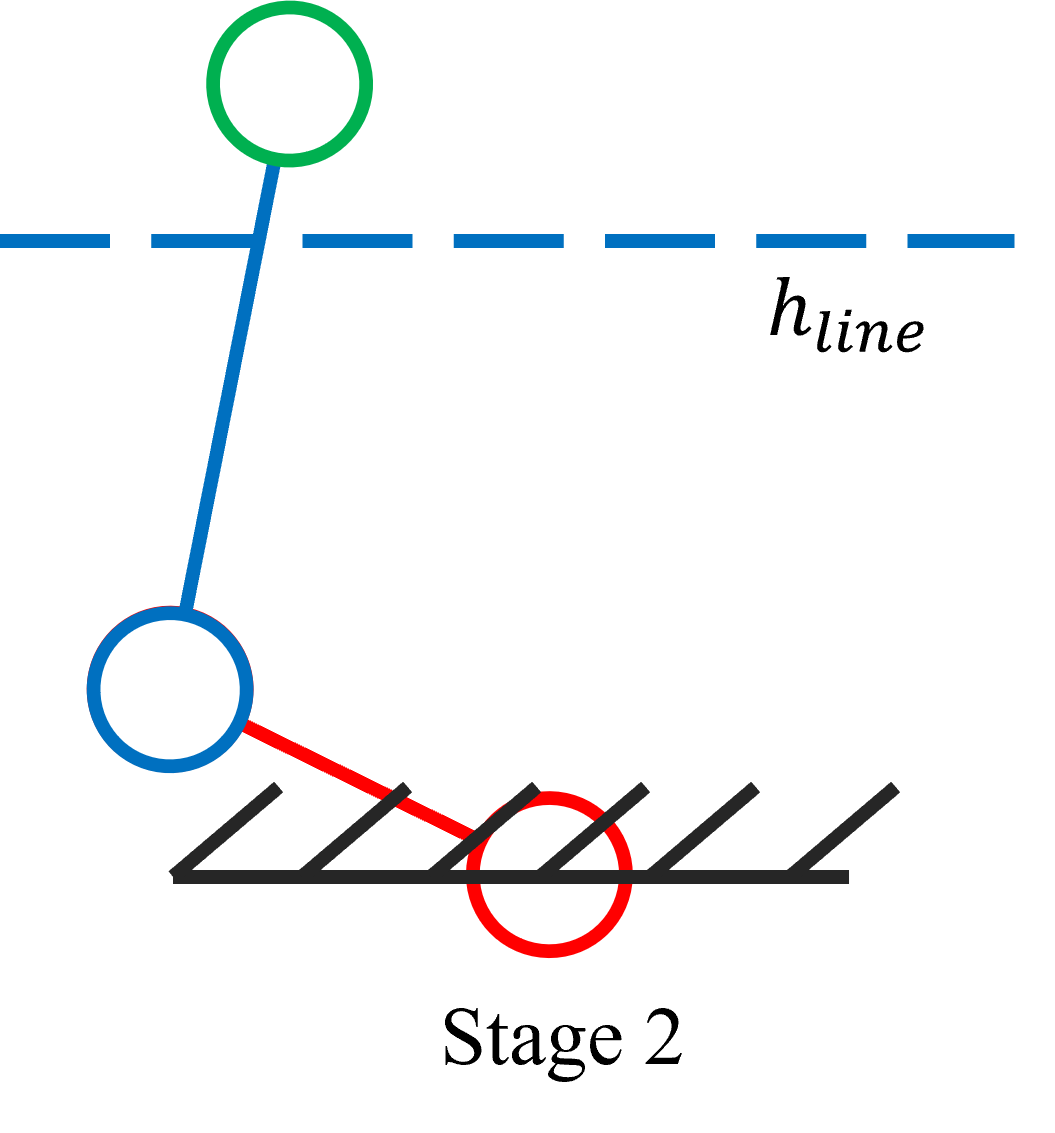
\includegraphics[width=0.25\textwidth]{figures/methodology/stage2.png} % Adjust the width as desired
    \caption{Swing up stage 2}
    \label{fig:stage2} % Optional label for referencing
\end{figure}

The third level of reward $r_{LQR}$ aims to provide a substantial reward to the
agent when it remains within the Region of Attraction (RoA) of the LQR
controller. By this we want to achieve that the policy learns to enter the LQR
controller RoA so that there can be a smooth transition between both
controllers.  The parameters, we used in
the cost matrices of the LQR controller are listed in
Table~\ref{tab:training_parameters}. 

\begin{figure}[H]
    \centering
    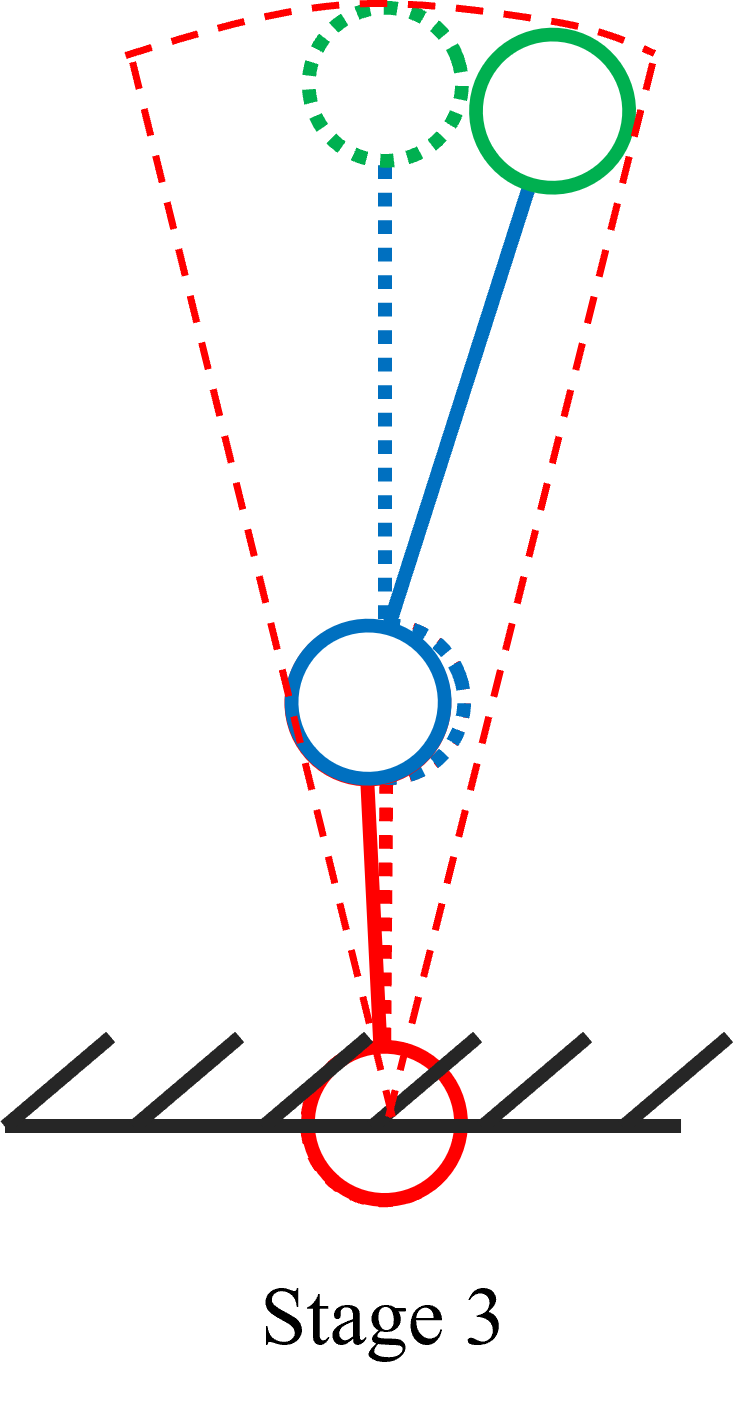
\includegraphics[width=0.2\textwidth]{figures/methodology/stage3.png} % Adjust the width as desired
    \caption{Swing up stage 3}
    \label{fig:stage3} % Optional label for referencing
\end{figure}


\section{Introduction to leaderboard metrics}
To facilitate a comparison of controller performance for the double pendulum testbench, three separate leaderboards have been created: the simulation leaderboard, the robustness leaderboard, and the real system leaderboard\cite{2023_ram_wiebe_double_pendulum}. Each of these leaderboards is additionally divided into two categories, which are determined by the pendubot and acrobot configurations.

\subsection{Performance Leaderboard in Simulation and Real system}
In the evaluation of controller performance, a set of metrics is utilized that extends beyond mere task success, delving into the finer aspects of controller operation. The same performance evaluation metrics are consistently applied to experiments conducted in both simulation environments and on real hardware. These metrics encompass various aspects, ranging from fundamental swing-up maneuver success to detailed examinations of energy consumption and torque utilization. Below, we provide a comprehensive breakdown of each metric:

\begin{itemize}
  \item \textbf{Swingup Success} \(c_{\text{success}}\):
  Determines if the end-effector successfully remains above the predefined threshold by the simulation's conclusion.
  
  \item \textbf{Swingup Time} \(c_{\text{time}}\):
  Measures the duration taken for the pendubot or acrobot to achieve and maintain its position above the threshold line. The metric only considers the swingup successful if the end-effector remains above the threshold until the simulation's end.
  
  \item \textbf{Energy} \(c_{\text{energy}}\):
  Quantifies the total mechanical energy expended during the task.
  
  \item \textbf{Max Torque} \(c_{\tau, \text{max}}\):
  Captures the highest torque applied at any point during the task.
  
  \item \textbf{Integrated Torque} \(c_{\tau, \text{integ}}\):
  Represents the cumulative torque applied throughout the task's duration.
  
  \item \textbf{Torque Cost} \(c_{\tau, \text{cost}}\):
  A quadratic metric that weighs the torques used, defined as \(c_{\tau, \text{cost}} = \sum u^TRu\), where \(R = 1\).
  
  \item \textbf{Torque Smoothness} \(c_{\tau, \text{smooth}}\):
  Reflects the variability or fluctuations in the torque signals by measuring their standard deviation.
  
  \item \textbf{Velocity Cost} \(c_{\text{vel, cost}}\):
  A metric assessing the joint velocities achieved, computed as \(c_{\text{vel}} = \dot{q}^T Q \dot{q}\), with \(Q\) being the identity matrix.
\end{itemize}

The cumulative RealAI Score is determined based on the specified formula, using the following criteria:

\begin{equation}
\begin{aligned}
S = c_{\text{success}} \Bigg(& w_{\text{time}}\frac{c_{\text{time}}}{n_{\text{time}}} + \\
& w_{\text{energy}}\frac{c_{\text{energy}}}{n_{\text{energy}}} +
w_{\tau, \text{max}}\frac{c_{\tau, \text{max}}}{n_{\tau, \text{max}}} +
w_{\tau, \text{integ}}\frac{c_{\tau, \text{integ}}}{n_{\tau, \text{integ}}} + \\
& w_{\tau, \text{cost}}\frac{c_{\tau, \text{cost}}}{n_{\tau, \text{cost}}} +
w_{\tau, \text{smooth}}\frac{c_{\tau, \text{smooth}}}{n_{\tau, \text{smooth}}} +
w_{\text{vel, cost}}\frac{c_{\text{vel, cost}}}{n_{\text{vel, cost}}} \Bigg)
\end{aligned}
\end{equation}

The weights and normalizations are:
\begin{table}[H]
  \centering
  \begin{tabular}{lcc}
    \hline
    Criteria & Normalization \(\mathit{n}\) & Weight \(\mathit{w}\) \\
    \hline
    Swingup time & 10.0 & 0.2 \\
    Energy & 100.0 & 0.1 \\
    Max. Torque & 6.0 & 0.1 \\
    Integrated Torque & 60.0 & 0.1 \\
    Torque Cost & 360 & 0.1 \\
    Torque Smoothness & 12.0 & 0.2 \\
    Velocity Cost & 1000.0 & 0.2 \\
    \hline
  \end{tabular}
  \caption{Weights and normalizations for performance leaderboards}
  \label{tab:performance}
\end{table}

In the simulation experiments, the pendubot is modeled using a Runge-Kutta 4 integrator with a timestep of \(dt=0.002s\) over a span of \(T=10s\). The pendubot is initiated in a hanging down configuration, represented as \(x_0 = [0, 0, 0, 0]^T\), with the goal of reaching the unstable fixed point in the upright configuration, denoted as \(x_g = [\pi, 0, 0, 0]^T\). The double pendulum is considered to have achieved its upright position once the end-effector surpasses the threshold line situated at \(h=0.45m\), with the origin being the mounting point.

In real hardware experiments, there exists a torque limit of 0.5 Nm on the passive joint, which compensates for the motor's friction. The actuators are capable of operating at a control frequency as high as 500Hz, and each experiment has a duration of 10 seconds. The pendubot commences from a hanging down position, aiming to reach the unstable fixed point in the upright configuration. Successful attainment of the upright position is confirmed when the end-effector crosses the threshold line set at \(h=0.45m\), measured from the mounting point's origin.

\subsection{Simulation Robustness Leaderboard}
In addition to performance metrics, we also consider robustness metrics. As the ultimate goal is to transfer successful models from a simulation environment to real hardware, it's essential to assess the robustness of controllers developed within the simulation. This helps determine the types of perturbations that affect each controller.

\begin{itemize}
    \item \textbf{Model Inaccuracies \(c_{model}\)}: Model parameters determined through system identification are inherently subject to inaccuracies. To assess these inaccuracies, variations are introduced one at a time into the independent model parameters within the simulator while maintaining the use of the original model parameters in the controller.

    \item \textbf{Velocity Measurement Noise \(c_{vel, noise}\)}: The outputs of the controllers depend on the measured system state, and in the case of the QDDs, online velocity measurements introduce noise. Therefore, it is important for transferability that a controller can handle at least this level of noise in the measured data. Testing is conducted with and without a low-pass noise filter.
    
    \item \textbf{Torque Noise \(c_{\tau,noise}\)}: Beyond measurement noise, the torque output by the controller may not precisely match the desired value.

    \item \textbf{Torque Response \(c_{\tau,response}\)}: The controller's requested torque typically varies during execution, and the motor may not be able to instantaneously respond to significant torque changes. Instead, it may overshoot or undershoot the desired torque value. This behavior is modeled by the equation \(\tau = \tau_{t-1} + k_{\text{resp}} (\tau_{\text{des}} - \tau_{t-1})\), where \(\tau_{\text{des}}\) is the desired torque. In this model, a \(k_{\text{resp}}\) value of 1 indicates flawless torque response, while any deviation from 1 indicates imperfect motor responses.

    \item \textbf{Time Delay \(c_{delay}\)}: In real-system operations, time delays inevitably arise due to communication and reaction times. It's essential to account for these when evaluating controller performance.
\end{itemize}

The above criteria are employed to compute the comprehensive RealAI Score using the given formula:
\begin{equation}
 S = w_{model} c_{model} + 
    w_{vel, noise} c_{vel, noise} +  
    w_{\tau, noise} c_{\tau, noise} +  
    w_{\tau, response} c_{\tau, response} +  
    w_{delay} c_{delay}
\end{equation}

The weights are:
\begin{equation}
 w_{model} = w_{vel, noise} = w_{\tau, noise} = w_{\tau, response} = w_{delay} = 0.2
\end{equation}
\cleardoublepage

\chapter{Experiment: agent training and simulation}
Chapters 4 and 5 focus on the experimental phase of our project. This chapter details the training procedure of our SAC agent for the swing-up task and then transitions to a simulation phase to validate results for both the swing-up and stabilization tasks. We have structured this chapter into three distinct subsections: training setup, training process, and simulation results.

The first subsection describes the foundation of a reinforcement learning interaction rooted in a stable baseline3-based RL algorithm. It also touches upon a customized environment inherited from the OpenAI Gym environment. The second subsection centers on hyperparameter tuning and highlights the challenges encountered during training. The third subsection displays the results acquired from both the pendubot and acrobot setups.

\section{Training setup}
Stable Baseline 3(SB3)\cite{stable-baselines3} is an open-source implementation of deep reinforcement learning algorithms based on the Python language. This library includes seven commonly used model-free deep reinforcement learning algorithms including SAC. Prior implementations of deep RL algorithms often encountered a problem wherein small implementation details could greatly affect performance, typically exceeding the differences between algorithms[some paper]. The developers of SB3 have done a commendable job stabilizing the performance of these deep RL algorithms by benchmarking each one on common environments and comparing them to prior implementations. Owing to its user-friendly and reliable nature, we chose Stable Baseline 3 as our RL library, which greatly simplified our research process.

OpenAI Gymnasium\cite{towers_gymnasium_2023} is a toolkit for developing and comparing reinforcement learning algorithms, and it is widely used in the research community. Among its many advantages are its open-source nature and standardized environments, which facilitate the rapid testing and benchmarking of new algorithms. Additionally, it offers easy visualization and monitoring. Our decision to use the Gym library is based on its extensibility—from standard environments to highly customized ones—as well as its capability to integrate with tools like PyTorch and TensorFlow for GPU-accelerated computations. Furthermore, Gym provides the ability to construct stacked training environments for parallel training.

\begin{figure}[htbp]
    \centering
    \includegraphics[width=0.7\linewidth]{example-image}
    \caption{Interaction between reinforcement learning agent and customized environment}
    \label{fig:my_label}
\end{figure}

To construct the customized environment, we begin with the symbolic dynamic function that captures the nonlinear dynamics of the underactuated double pendulum. This function uses the current state observation from the simulation and the action determined by the control policy, producing a prediction of the next state via a Runge-Kutta integrator.

This predicted state is then input into the reward function, which yields a scalar output. This output is subsequently relayed to the SAC algorithm for policy evaluation and update. After these computations, the simulation provides an estimation of the current state, and the policy identifies the most probable action. Both of these values are then directed back to the dynamics function, initiating a new cycle.

It's widely recognized that reinforcement learning algorithms tend to converge more effectively when using normalized state and action spaces \cite{sutton2018reinforcement}. Therefore, we've designed a scaling mechanism to translate the state and action spaces from their normalized versions to real-world measurements. Users can choose to activate or deactivate this scaling. For example, while a normalized state resides within the interval \( [-1,1] \), we might wish to map it to real-world measurements \( \left[ \text{pos1}, \text{pos2}, \text{vel1}, \text{vel2} \right] \), such as \( \text{pos1} \) in \( [0,2\pi] \), \( \text{pos2} \) in \( [-\pi,\pi] \), and velocities \( \text{vel1} \) and \( \text{vel2} \) in \( [-20,20] \) rad/s, while keeping the torque within \( [-\tau_{\text{limit}}, \tau_{\text{limit}}] \). When this scaling mechanism is activated, it ensures that states and actions in the SAC algorithm always stay within the \( [-1,1] \) boundary, which often leads to faster convergence. The mapping relation of the scaling mechanism is demonstrated in the picture below:

\begin{figure}[H]
    \centering
    \includegraphics[width=0.7\linewidth]{example-image}
    \caption{mapping relation of the scaling mechanism}
    \label{fig:my_label}
\end{figure}

The logic of the pipeline of the interaction of customized environment is described in the picture below.

\begin{figure}[H]
    \centering
    \includegraphics[width=0.7\linewidth]{example-image}
    \caption{logic of the interaction}
    \label{fig:my_label}
\end{figure}

or

\begin{algorithm}
\caption{Customized environment}
\begin{algorithmic}[1]
\Procedure{Euclid}{$a,b$}
\While{$b \neq 0$}
    \State $t \gets b$
    \State $b \gets a \mod b$
    \State $a \gets t$
\EndWhile
\State \textbf{return} $a$
\EndProcedure
\end{algorithmic}
\end{algorithm}

\section{Training phase}
The training phase started immediately after we finished setting up the training pipeline. During the training of the SAC controller for both the acrobot and pendubot, our primary focus was on tuning several key hyperparameters. These encompassed the learning rate, control frequency, episode length, and learning timestep. We invested much effort in adjusting hyperparameters for the reward function and the LQR controller, given their pivotal roles in the learning process, as detailed in Table 4.1.

We set the learning rate at 0.01 to promote effective learning and adaptation. Additionally, we configured the control frequency of the simulation to 100Hz, ensuring frequent updates and heightened responsiveness in the control process. We selected an episode length of 1000 for both the Acrobot and Pendubot, translating to 10-second-long episodes, to provide sufficient exploration and learning opportunities. To harness the full training potential, we executed a total of 2e7 learning time steps for the pendubot and 5e7 for the acrobot, allowing the agent to accumulate vast experience and enhance its performance.


\begin{table}[H]
  \centering
  \begin{tabular}{p{2cm} | p{3cm} | p{3cm} | p{3cm}}
  Robot & Quadratic Reward  & Constant Reward & LQR\\
  \hline
  \multirow{5}{*}{Pendubot} & \(Q_1\) = 8.0  &  & \(Q_1\) = 1.92\\
  & \(Q_2\) = 5.0  & \(r_{line}=500\) & \(Q_2\) = 1.92\\
  & \(Q_3\) = 0.1  & \(r_{vel}=0.0\) & \(Q_3\) = 0.3\\
  & \(Q_4\) = 0.1  & \(r_{LQR}=1e4\)& \(Q_4\) = 0.3\\
  & \(R\) = 1e-4  & & \(R\) = 0.82\\
  \hline
  \multirow{5}{*}{Acrobot} & \(Q_1\) = 10.0  &  & \(Q_1\) = 0.97\\
  & \(Q_2\) = 10.0  & \(r_{line}=500\) & \(Q_2\) = 0.93\\
  & \(Q_3\) = 0.2  & \(r_{vel}=1e4\) & \(Q_3\) = 0.39\\
  & \(Q_4\) = 0.2  & \(r_{LQR}=1e4\) & \(Q_4\) = 0.26\\
  & \(R\) = 1e-4  &  & \(R\) = 0.11\\
  \end{tabular}
 \caption{Hyper parameters used for the SAC training and the LQR controller.}
 \label{tab:parameters}
\end{table}

The learning curve for a total of 2e7 timesteps for the pendubot is illustrated below.As depicted in the figure, from 0 to 1e7 timesteps, the learning curve experiences a gradual ascent. Between 1e7 and 1.2e7 timesteps, the learning curve surges rapidly, peaking in reward around one million. After 1.2e6 timesteps, the curve begins to stabilize with occasional fluctuations, and no substantial increase in reward is observed.

\begin{figure}[H]
    \centering
    \fbox{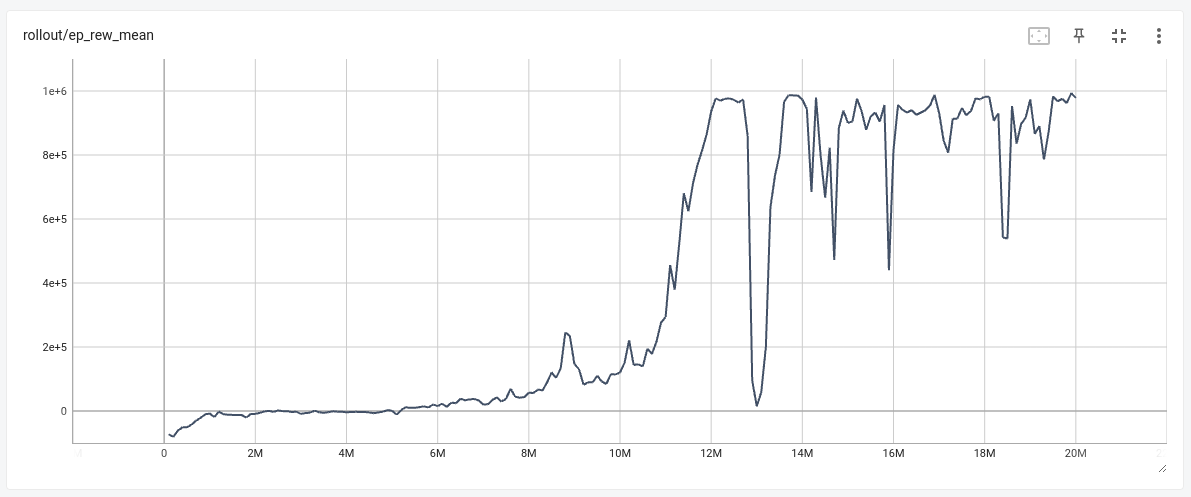
\includegraphics[width=0.9\textwidth]{figures/learning_curve/pendubot_learning_curve.png}} % First image
    \caption{pendubot learning curve}
    \label{fig:image_a}
\end{figure}

As shown in the learning curve over a total of 3e7 timesteps for the acrobot, the curve experienced a relatively steady growth until 1.8e7 timesteps. After a sudden drop in reward between 1.8e7 and 2e7 timesteps, the learning curve began to increase drastically, with two major fallbacks. By 3e7 timesteps, the learning curve hadn't reached its peak. We extended the learning period to 5e7 using a warm start from the model obtained at 3e7 timesteps, and the learning curve began to stabilize around 4e7 time steps.

\begin{figure}[H]
    \centering
    \fbox{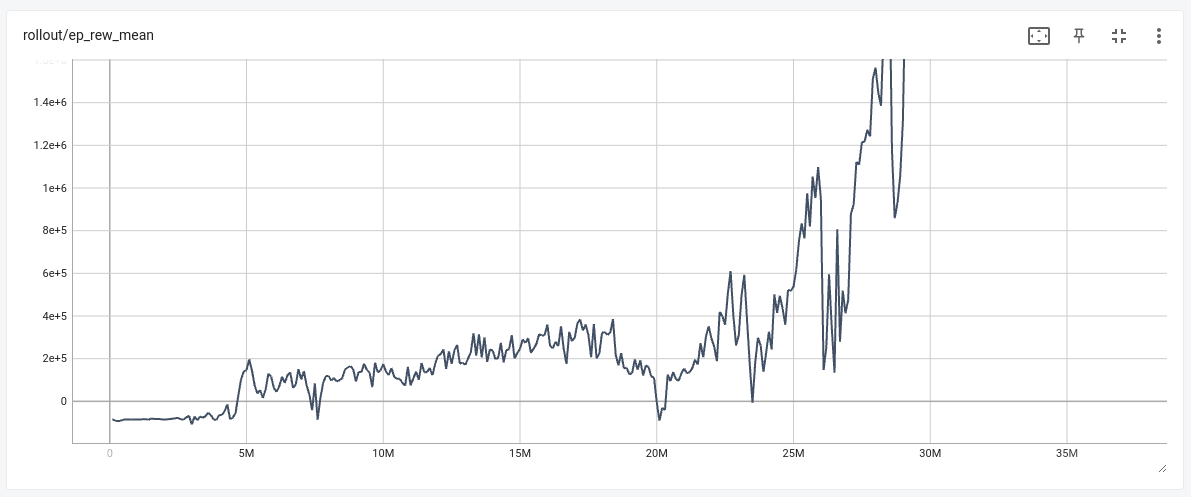
\includegraphics[width=0.9\textwidth]{figures/learning_curve/acrobot_learning_curve.png}} % Second image
    \caption{acrobot learning curve}
    \label{fig:image_b}
\end{figure}

In conclusion, the training for the pendubot converges more quickly than that for the acrobot. Additionally, based on the training curves, the pendubot's training process is more stable than the acrobot's.

\section{Simulation results}
In this section, the simulation results for the acrobot and pendubot are presented separately. The model trained using the SAC algorithm is utilized during the swing-up stage and switches to the LQR controller when nearing the upright position. The primary success criteria for both swing-up and stabilization involve swinging up the double pendulum and maintaining its stability around the upright position for a prolonged period. Therefore, a total simulation time of 10 seconds is used. If the double pendulum fails to swing up within these 10 seconds, the result is deemed unsuccessful. Similarly, if the double pendulum loses stability within this time frame, the outcome is still considered a failure.

\subsection{Pendubot simulation in ideal environment}
A testing environment, identical to the customized learning environment, has been established to validate the training results and accurately replicate the agent's behavior learned during the reinforcement learning process. The pendulum is initialized at its lowest point with zero velocity and begins its swing-up using the control policy derived solely from the SAC.

As depicted in the figure, the swing-up time is under 1 second. After this, the state of the pendubot enters the Region of Attraction (ROA) of the LQR controller. The transition between the two controllers is both seamless and effective, with the system stabilizing towards the desired state under the LQR controller's influence. This validates the effectiveness of the ROA method for the LQR takeover.

A significant highlight from this successful simulation is the impressively short swing-up time, despite having strict torque limit in place. However, a concerning feature observed from this simulation is the noisiness of the input control signal. The torque alternates signs rapidly, and the gradient of the torque tends to have a high absolute value.

\begin{figure}[H]
    \centering
    \fbox{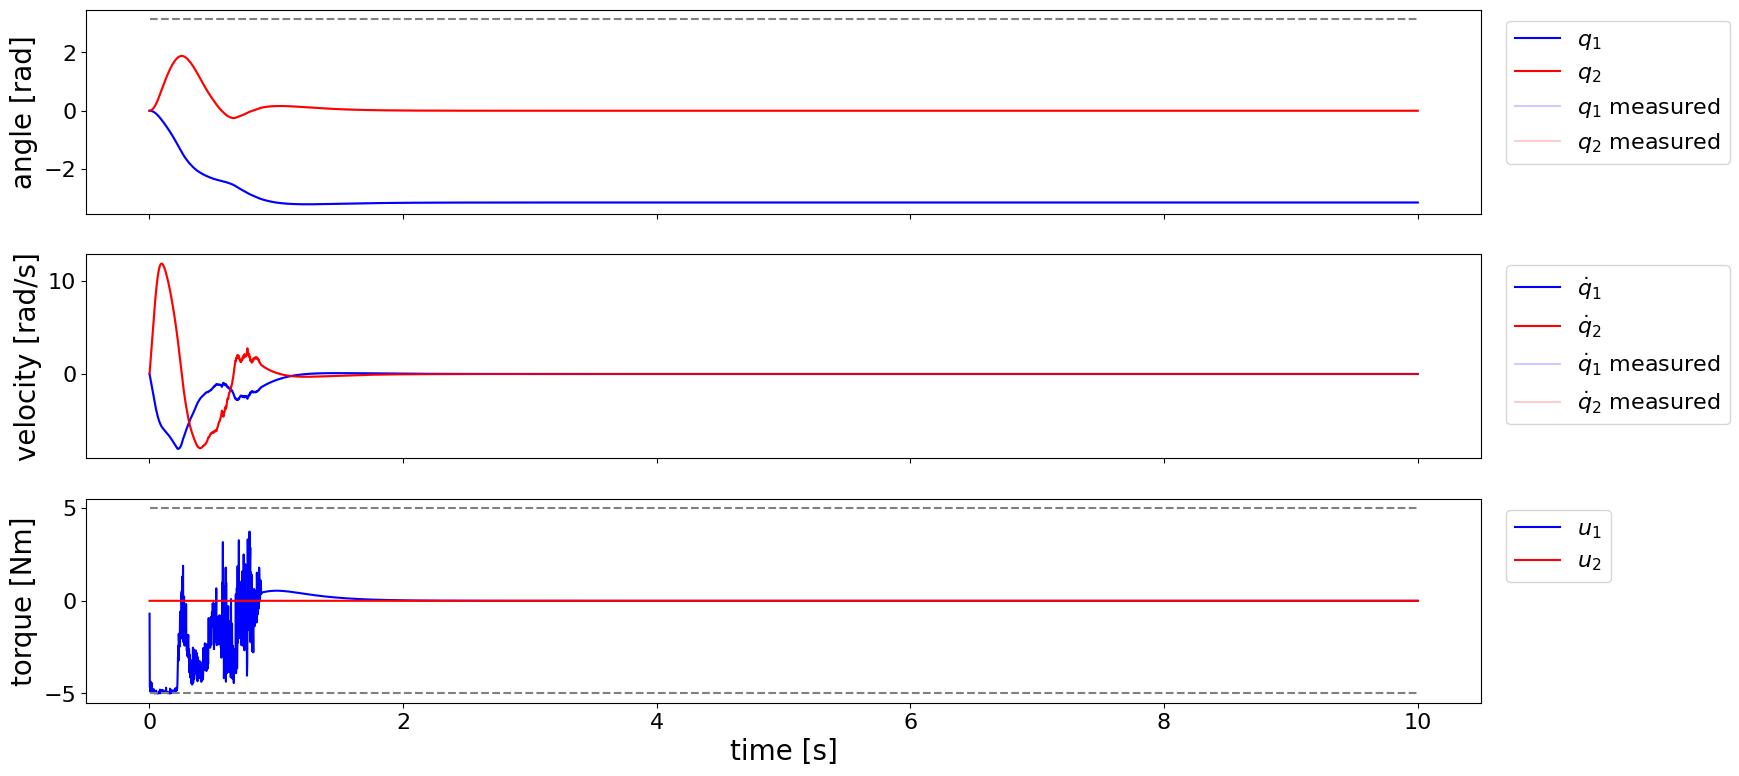
\includegraphics[width=0.9\textwidth]{figures/simulation_result/pendubot_unclipped.png}} % First image
    \caption{pendubot simulation result}
    \label{fig:image_a}
\end{figure}

\subsection{Acrobot simulation in ideal environment}

Just like the pendubot simulation, the acrobot setup is tested in an ideal environment identical to its training environment. The acrobot begins its swing from the downward position with the goal of stabilizing around its highest point.

The accompanying image depicts a successful swing-up and stabilization within a 10-second window. The swing-up process takes about 2 seconds before the LQR effectively assumes control, maintaining an asymptotic stability around the target state with minimal fluctuations.

In comparison to the pendubot's simulation curves, the swing-up time for the acrobot is roughly twice as long. This aligns with the notion that controlling the acrobot is a more challenging task than the pendubot. A shared drawback observed in both simulations is the lack of torque smoothness. For the acrobot, the input torque exhibits several significant jumps from one torque limit to the other, which might cause difficulties when translating to real-world hardware control.

\begin{figure}[htbp]
    \centering
    \fbox{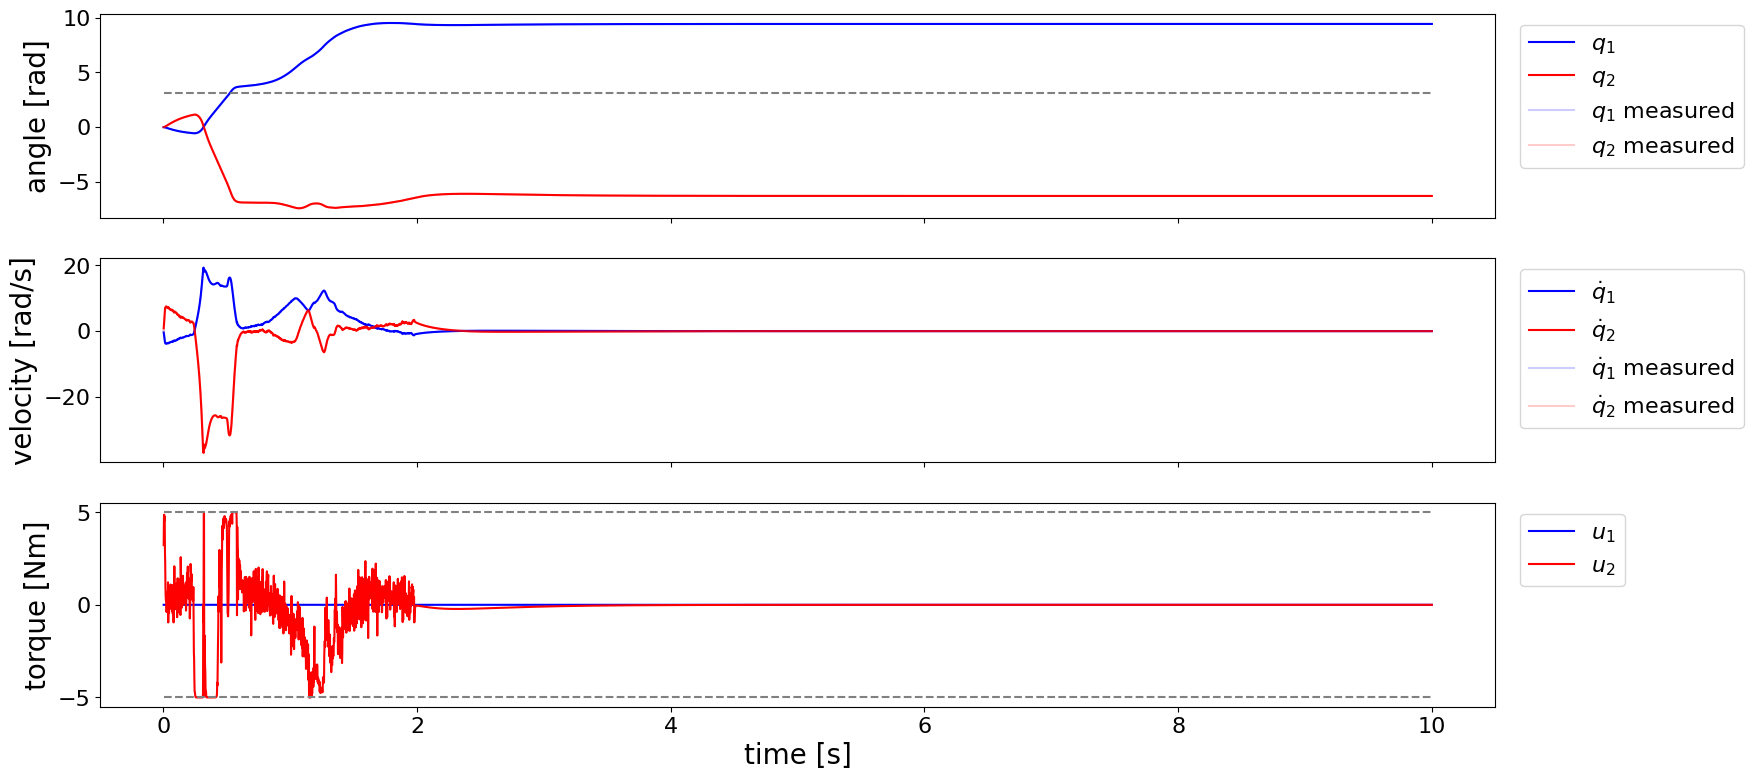
\includegraphics[width=0.9\textwidth]{figures/simulation_result/acrobot_unclipped.png}} % Second image
    \caption{acrobot simulation result}
    \label{fig:image_b}
\end{figure}


\cleardoublepage

\chapter{Experiments on real hardware}
In this chapter, the experiments conducted on the hardware system are discussed. The content is organized into four sections. An overview of the hardware setup for the double pendulum system is provided in the first section. The system identification of the hardware is delved into in the second section. The approach to addressing the sim-to-real gap challenge is detailed in the third section. The outcomes of the hardware experiments are presented in the final section.

\section{Hardware setup}
To be clear upfront, the hardware design and manufacturing were completed by previous researchers and coworkers at the Underactuated Lab of the German Research Center for Artificial Intelligence GmbH, Robotics Innovation Center branch. My role in this section is to understand the logic of all the involved subsystems and set up the test environment using existing components.

Mechanically, the double pendulum system is a straightforward 2-R linkage. The first revolute joint attaches to the base, while the second one connects the two links. Quasi-direct drive motors are mounted on each joint to provide torque, and a counterweight is positioned at the end of the second link.

The mechanical design of the double pendulum underwent two iterations. The initial design was characterized by rotational imbalances due to a slightly misaligned motor axis and homogeneous link sizes, leading to vibrations and potential failures. Significant improvements were made in the second iteration: the original aluminum-plastic links were replaced with a carbon fiber-foam composite, and a lightweight, triangular design with central cutouts was introduced. These changes not only rectified the weaknesses of the previous design but also resulted in a mechanical structure that was markedly more reliable and safer, with enhanced yield strength and reduced safety risks.

\begin{figure}[H]
    \centering
    \begin{subfigure}[b]{0.3\textwidth}
        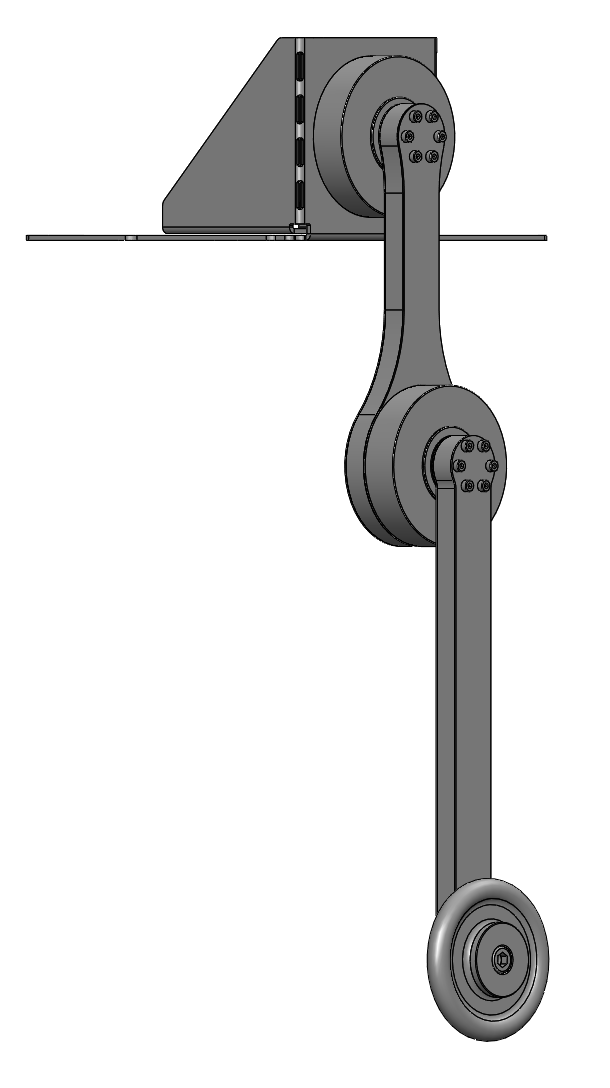
\includegraphics[width=\textwidth]{figures/hardware_setup/double_pendulum_it1_v1.png}
        \caption{Iteration 1 in isometric view}
        \label{fig:image1}
    \end{subfigure}
    \hfill
    \begin{subfigure}[b]{0.3\textwidth}
        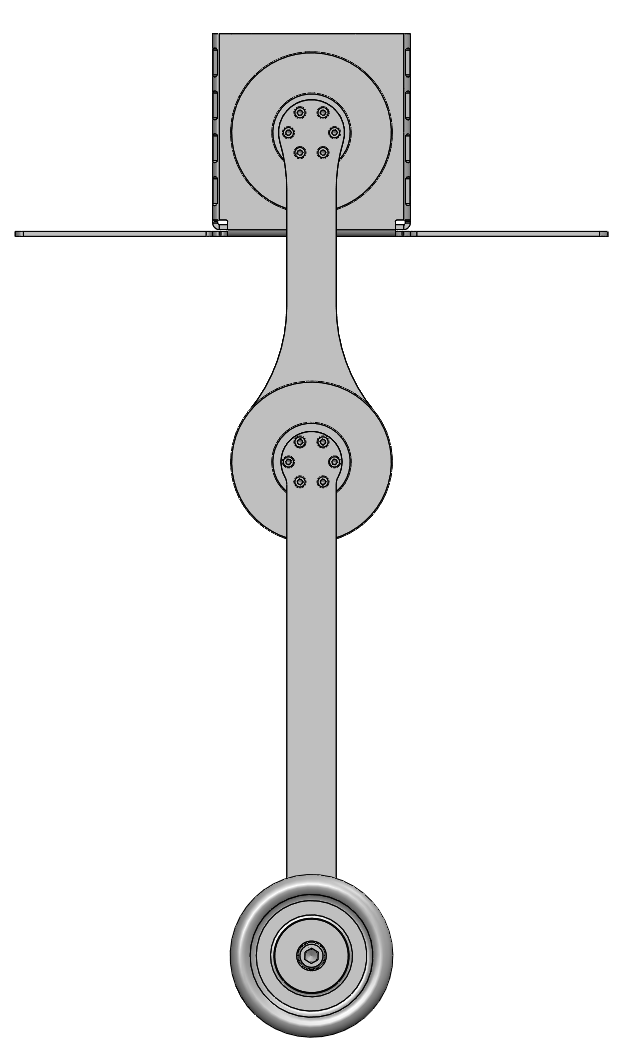
\includegraphics[width=\textwidth]{figures/hardware_setup/double_pendulum_it1_v2.png}
        \caption{Iteration 1 in front view}
        \label{fig:image2}
    \end{subfigure}

    \vspace{1em} % or use \bigskip or \medskip depending on the space you want

    \begin{subfigure}[b]{0.3\textwidth}
        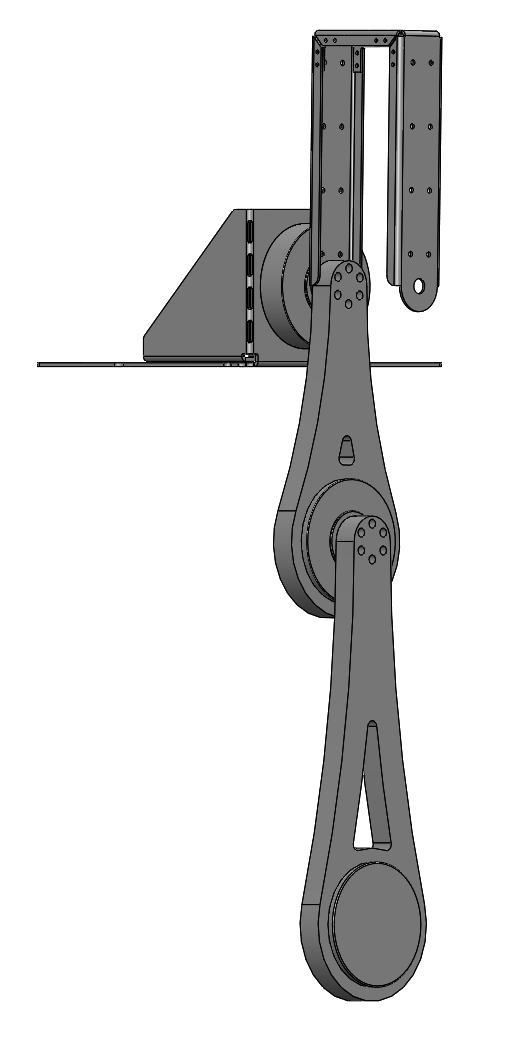
\includegraphics[width=\textwidth]{figures/hardware_setup/double_pendulum_it2_v1.png}
        \caption{Iteration 2 in isometric view}
        \label{fig:image3}
    \end{subfigure}
    \hfill
    \begin{subfigure}[b]{0.3\textwidth}
        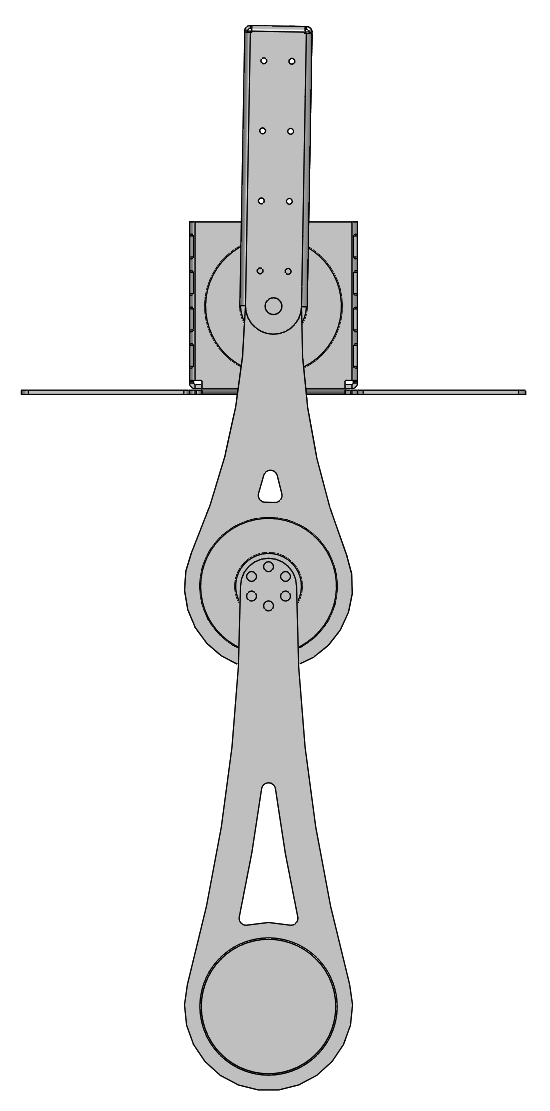
\includegraphics[width=\textwidth]{figures/hardware_setup/double_pendulum_it2_v2.png}
        \caption{Iteration 2 in front view}
        \label{fig:image4}
    \end{subfigure}
    \caption{Double pendulum mechanical system iteration 1 and iteration 2}
    \label{fig:four_images}
\end{figure}

For actuation selection, quasi-direct drive (QDD) motors were chosen. QDDs are popular choices for actuation in robotics, commonly utilized in applications that demand both high torque and precise control, such as robotic arms or exoskeletons. They represent a compromise between direct drive systems, which connect the load directly to the motor without any gear reduction, and traditional geared systems, which use gears to increase torque at the cost of speed and may introduce backlash. The advantages of employing QDDs are apparent: they offer high precision and allow for precise control. Furthermore, the low gear ratio simplifies joint dynamics, which can typically be neglected when modeling the overall system dynamics. The drawbacks, however, are also evident. QDDs are costlier than average motors, and the low gear ratio limits the torque output.

\begin{figure}[H]
  \centering
  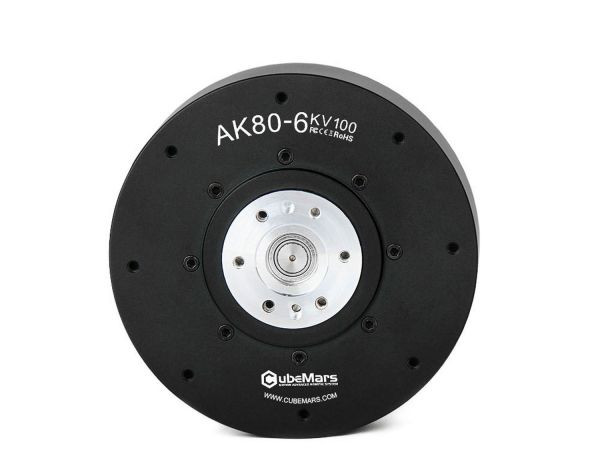
\includegraphics[width=0.5\textwidth]{figures/hardware_setup/motor.jpg}
  \caption{AK80-6 V100 motor\cite{cubemarsAK806}}
  \label{fig:AK80-6}
\end{figure}

The AK80-6 V100 motors from CubeMars were selected for their ease of mounting, which is facilitated from both the front and rear ends\cite{cubemarsAK806}. As shown in Figure \ref{fig:torque_speed_curve}, these motors are characterized by a peak torque of 12 Nm and a rated torque of 6 Nm during continuous operation, aligning with the project's set torque limit of 5 Nm. They are designed to operate on a 24V voltage with a gear ratio of 6:1. Additionally, their design incorporates compatibility with both serial and CAN bus systems, which simplifies the development process.

\begin{figure}[H]
  \centering
  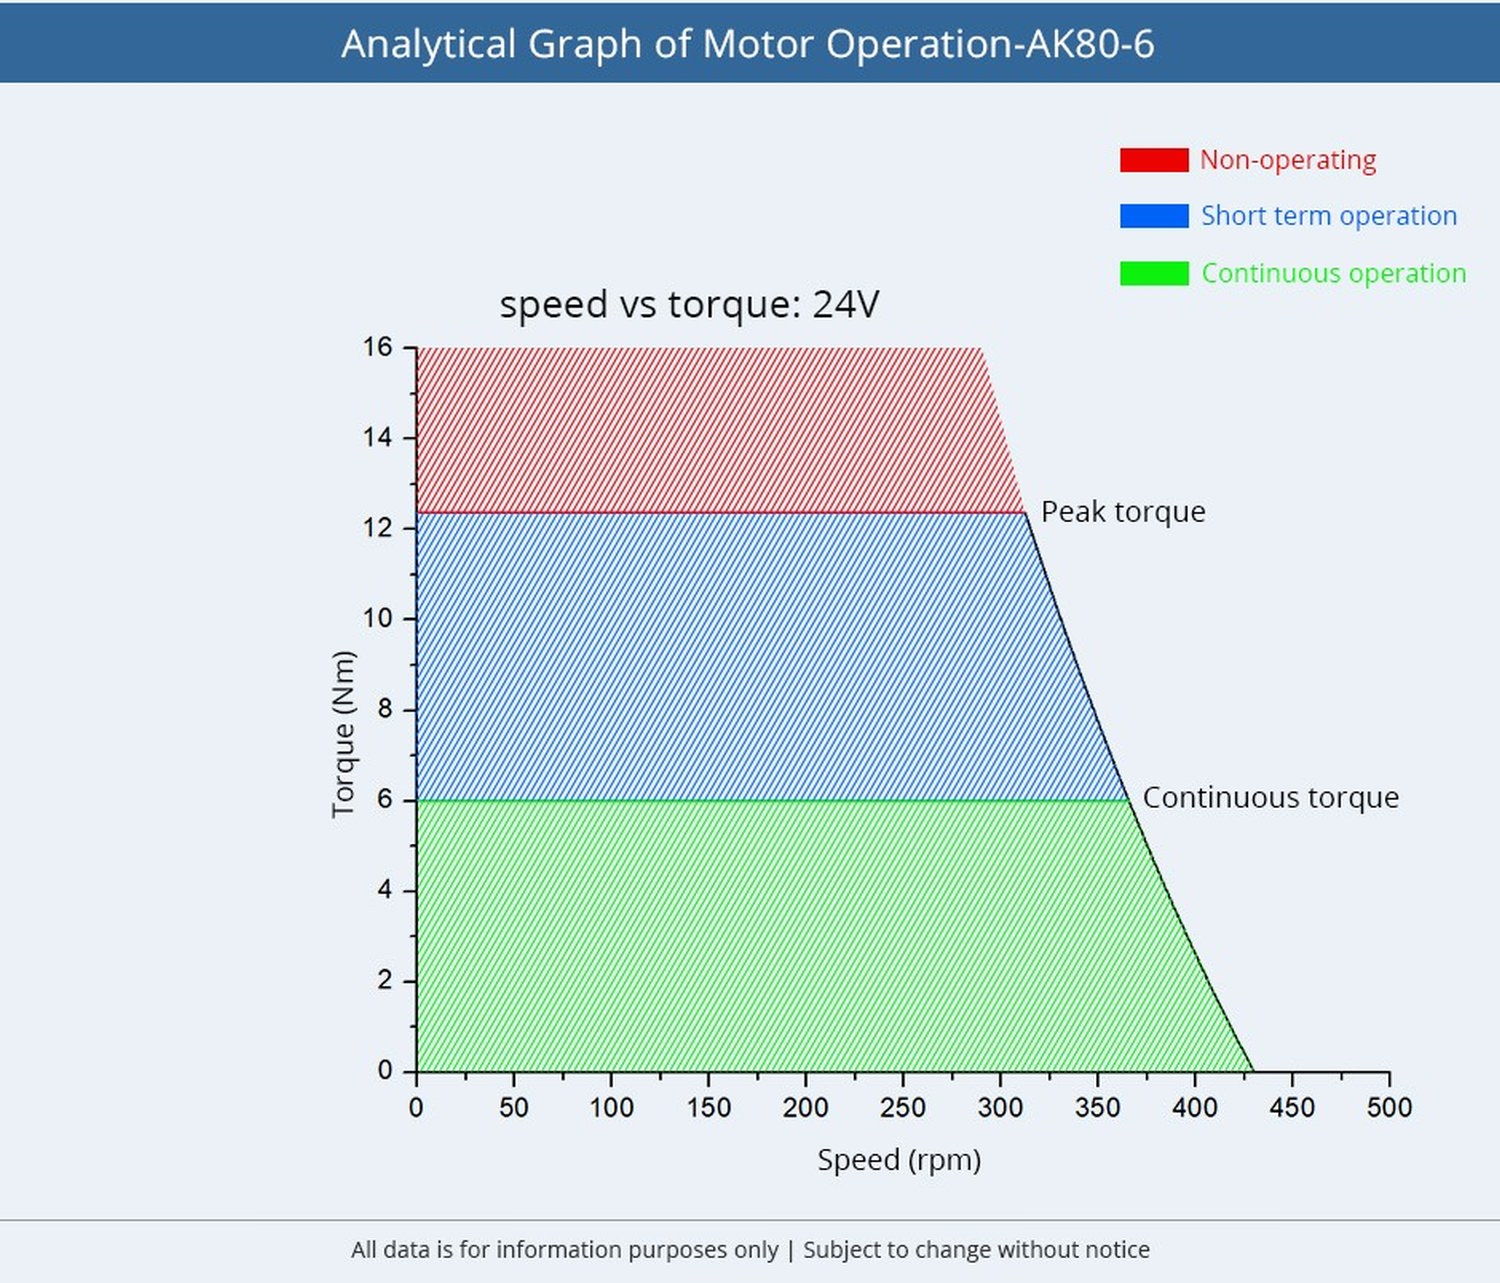
\includegraphics[width=0.80\textwidth]{figures/hardware_setup/torque_speed_curve.jpg}
  \caption{Torque speed curve of AK80-6 V100 motor\cite{cubemarsAK806}}
  \label{fig:torque_speed_curve}
\end{figure}

For communication, the Controller Area Network (CAN) bus was chosen due to its compatibility with the actuators. Known for its robustness, flexibility, and efficiency, the CAN bus is a communication protocol that has been widely utilized in various applications. The adoption of the CAN bus for control brings numerous advantages. It provides error checking and fault confinement capabilities and supports real-time operation, facilitating high control frequencies with a relatively simple wiring arrangement. 

In our application (Figure \ref{fig:can_connection_diagram}), the network comprises one master node (the PC) and two slave nodes (the motors). The control loop is constituted by a CAN-to-USB converter, a single CAN high cable, and a single CAN low cable, with termination resistors of \(120 \Omega\) at both the initial and terminal points of the network.

\begin{figure}[H]
  \centering
  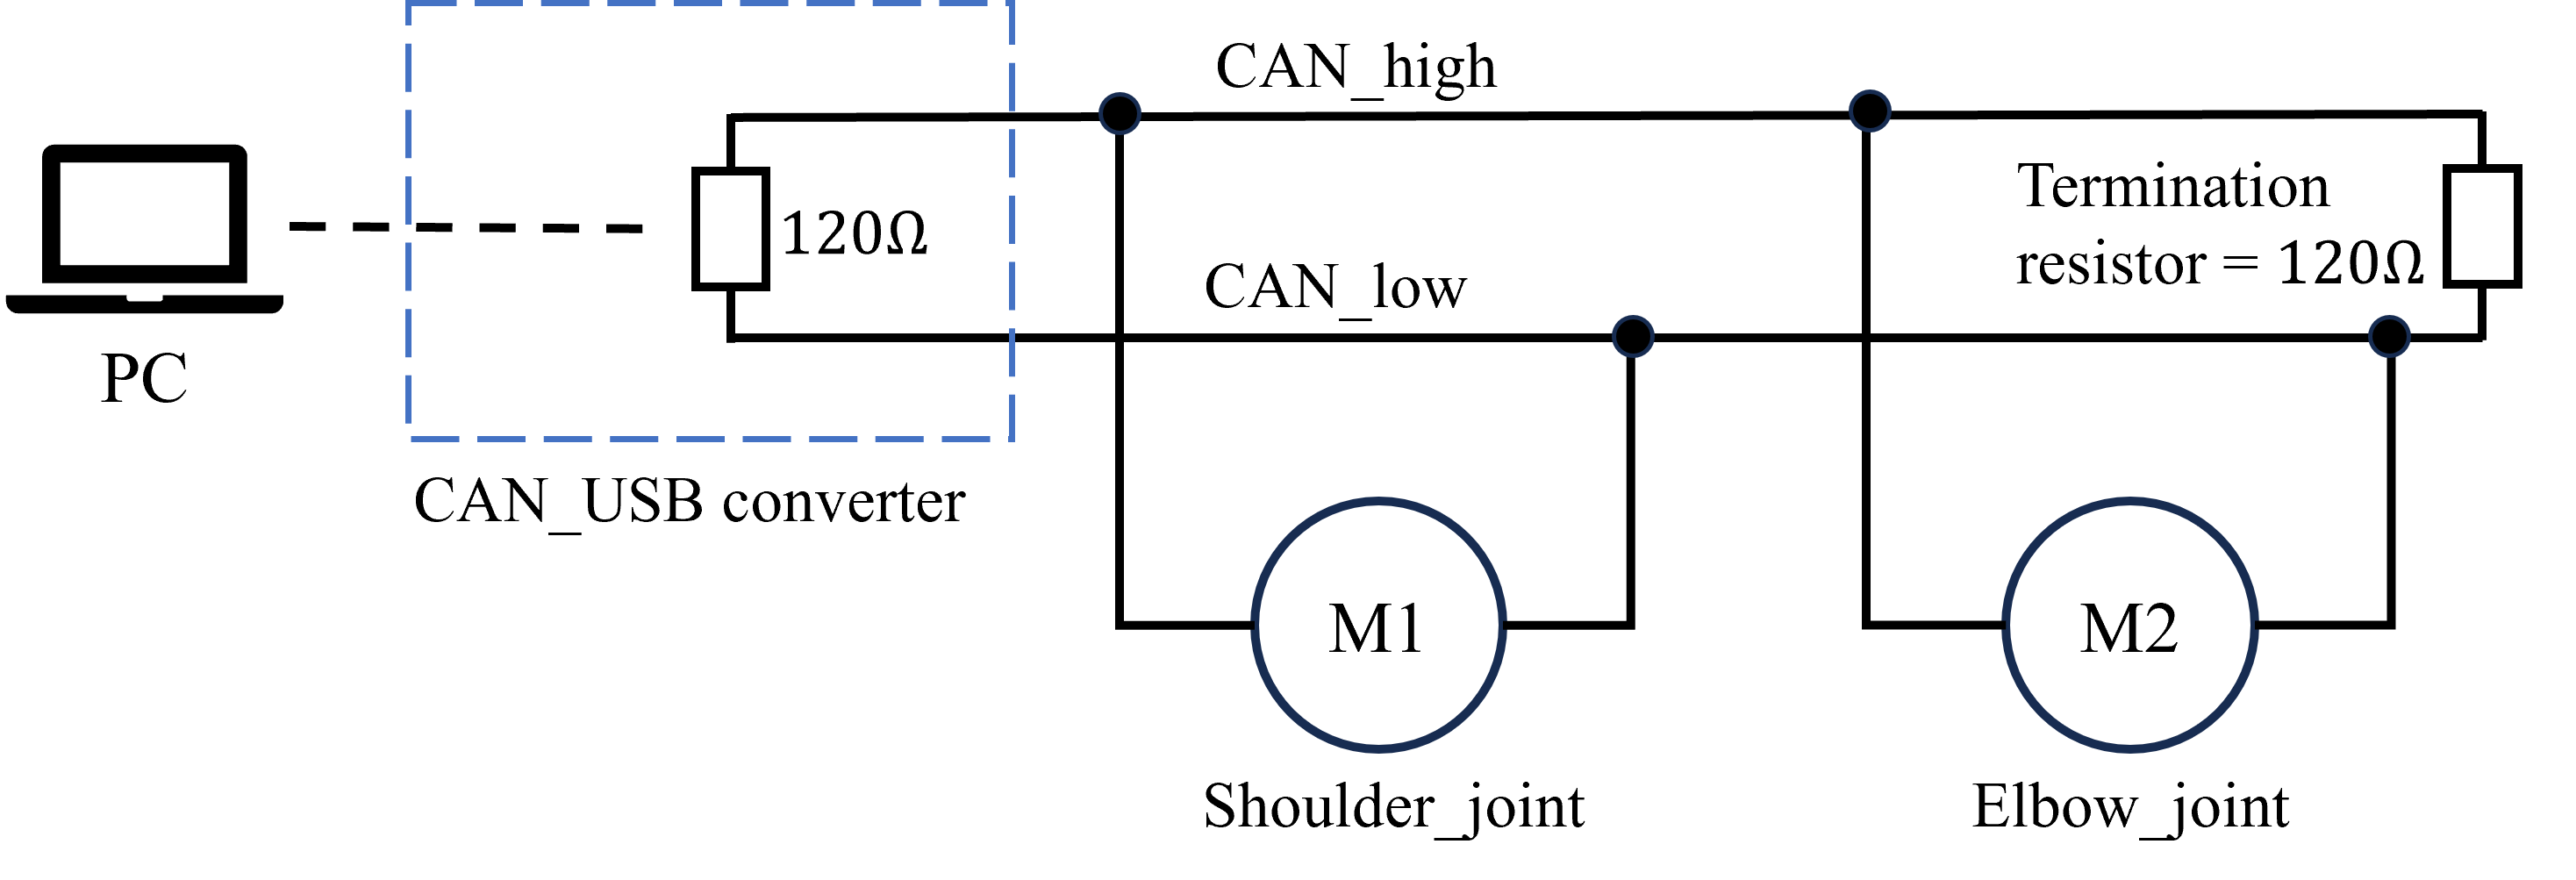
\includegraphics[width=0.9\textwidth]{figures/hardware_setup/can_connection.png}
  \caption{CAN connection diagram}
  \label{fig:can_connection_diagram}
\end{figure}

To achieve a higher control frequency of approximately 500 Hz, the CAN-USB/2 product from ESD GmbH Hannover~\cite{esdCANUSB2} was selected. This specialized interface exploits the USB 2.0 standard, which allows for a data rate of 480 Mbit/s, and features CAN capability at 1 Mbit/s as per ISO 11898-2. Furthermore, compatibility with the SocketCAN interface, which is incorporated into the Linux Kernel 2.6, is supported, thereby facilitating its use within a Linux development environment.

\begin{figure}[H]
    \centering
    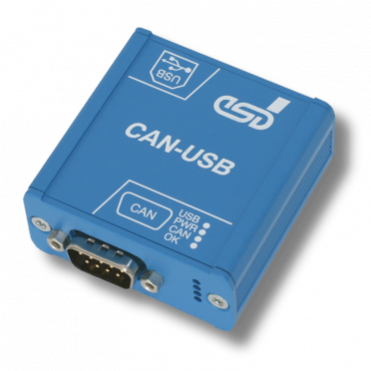
\includegraphics[width=0.3\linewidth]{figures/hardware_setup/can_blue_box.png}
    \caption{High speed CAN to USB interface\cite{esdCANUSB2}}
    \label{fig:can_blue_box}
\end{figure}

Following accidents encountered during testing with the initial mechanical systems, several safety protocols have been instituted to safeguard human lives and equipment. Four principal measures are now in place.

\textbf{Emergency stop:}

An emergency stop has been interfaced directly with the 24V power supply. In the event that the double pendulum's behavior deviates from the expected parameters during tests, the power can be disconnected manually with immediate effect. Subsequently, the mechanical system's energy will dissipate swiftly, causing an automatic reversion to its initial state.

\textbf{Capacitor:}

In instances where the emergency stop is activated while the system operates at high velocities, the motors at the revolute joints serve as generators, converting the mechanical energy into electrical energy. This conversion process results in a current that is channeled back into the circuit, which, under extreme conditions, has the potential to overload the power supply. To mitigate this, a capacitor has been incorporated into the power supply circuitry to capture any excessive electrical energy that may arise from the abrupt cessation of the system's movement.

\begin{figure}[H]
    \centering
    \includegraphics[width=0.4\textwidth]{figures/hardware_setup/capacitor.jpg}
    \caption{Capacitor}
    \label{fig:capacitor}
\end{figure}

\textbf{Speed and position limit:}

At the software level, speed and position limits have been defined. Due to the potential for vibrations and rotational imbalances that may occur at high speeds, which could lead to structural disassembly, a maximum speed of \(20\) rad/s has been instituted. Should the speed surpass this threshold, an automatic system halt will be initiated, analogous to the actuation of the emergency stop mechanism. Position limits have been established at \(2\pi\) for both joints. Excessive rotations risk the entanglement of CAN and power cables, which could result in interference and possible cable damage. A schematic of the entire wiring system is illustrated in the Figure \ref{fig:wiring diagram}:

\textbf{Physical enclosure:}

A custom-designed enclosure(see Figure \ref{fig:overview_experiment_setup}) has been fabricated to serve as a safeguard against unanticipated system failures. Constructed from aluminum profiles and reinforced with thick acrylic boards, the enclosure comprehensively surrounds the double pendulum apparatus, significantly mitigating the potential for accidents.

These safety measures have been crucial in reducing the risks associated with testing and operational procedures.

\begin{figure}[H]
    \centering
    \includegraphics[width=0.9\textwidth]{figures/hardware_setup/enclosure.jpg}
    \caption{Physical enclosure for protection}
    \label{fig:overview_experiment_setup}
\end{figure}

\begin{figure}[H]
    \centering
    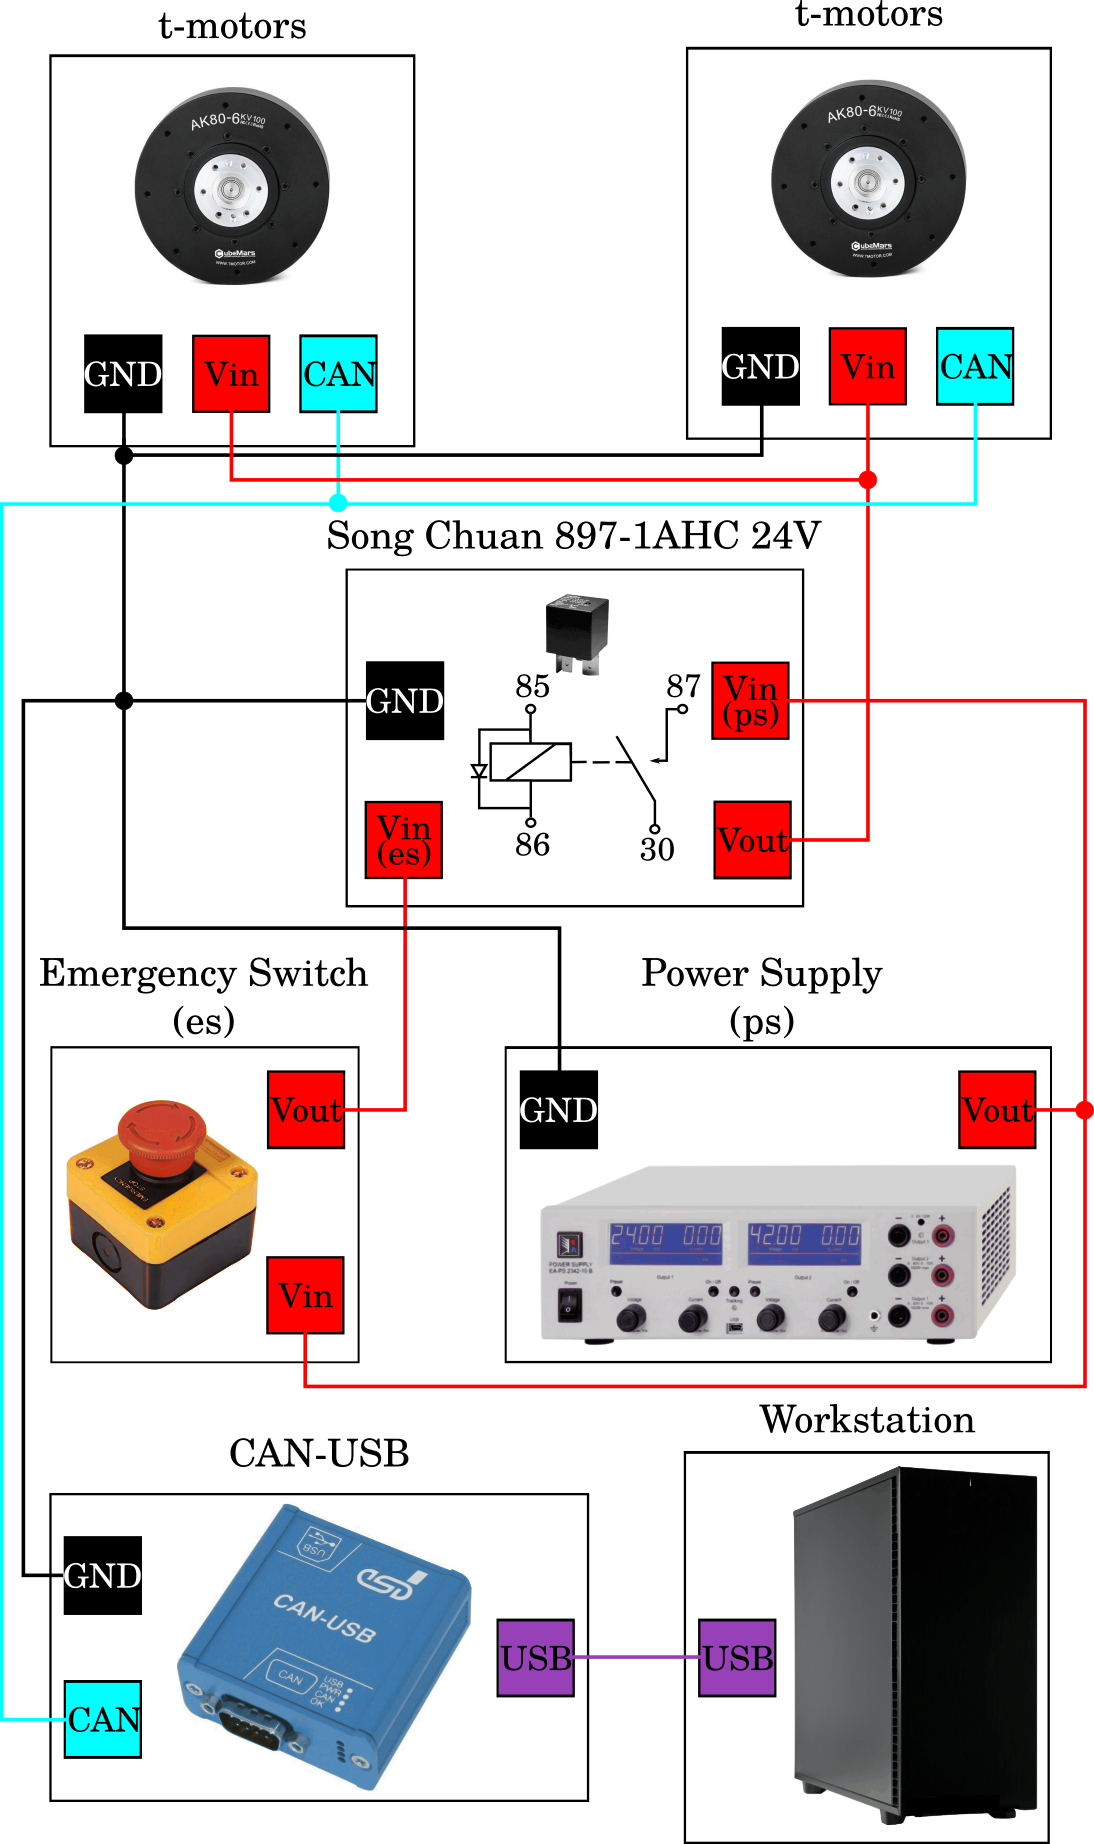
\includegraphics[width=0.7\linewidth]{figures/hardware_setup/wiring-diagram.png}
    \caption{Wiring diagram\cite{2023_ram_wiebe_double_pendulum}}
    \label{fig:wiring diagram}
\end{figure}

\section{System identification}
Before implementing control strategies on a real system, it is crucial to ensure that the dynamics of the real system match those anticipated in theory. To achieve this, identifying the values used in the equation of motion is essential, and the system identification method is employed.

System identification is the process of deriving mathematical models of dynamic systems from observed input-output data. This method is widely used in control theory to analyze and predict the behavior of real-world systems. The common procedure of system identification includes model structure selection, data collection, and parameter estimation.

\textbf{Model Structure Selection:}

As described in Section 2.1.2, the equation of motion for the target system is derived using the Lagrangian method, as expressed in Equation \ref{eq:EoM}. Fifteen parameters are required to fully describe the system dynamics, including masses $(m_1, m_2)$, lengths $(l_1, l_2)$, centers of masses $(r_1, r_2)$, inertias $(I_1, I_2)$ for the two links, and six actuator parameters, namely motor inertia $I_r$, gear ratio $g_r$, Coulomb friction $(c_{f1}, c_{f2})$, and viscous friction $(b_1, b_2)$ for the two joints, and gravity $g$.

While the naturally provided parameters $g$ and $g_r$ are held constant, the easily measurable parameters $l_1$ and $l_2$ are measured by hand and recorded in Table \ref{tab:different_designs}. The remaining 11 system parameters need to be determined. We define the following terms as independent variables, which are to be estimated during the system identification experiment:

\[m_1 r_1, m_2 r_2, m_1, m_2, I_1, I_2, I_r, b_1, b_2, c_{f1}, c_{f2}\]

\textbf{Data Collection:}

System identification experiments are conducted by running excitation trajectories on the real hardware. The excitation trajectories include inputs of $[t, q, \dot{q}, \ddot{q}]^T$, where $t$ is the timestamp, $q = [p_1, p_2]^T$ represents position, $\dot{q} = [v_1, v_2]^T$ represents velocity, and $\ddot{q} = [a_1, a_2]^T$ represents acceleration. Data tuples in the form $(q, \dot{q}, \ddot{q}, u)$ can be collected. One of the excitation trajectories are shown in Figure \ref{fig:excitation_traj}.

\begin{figure}[H]
    \centering
    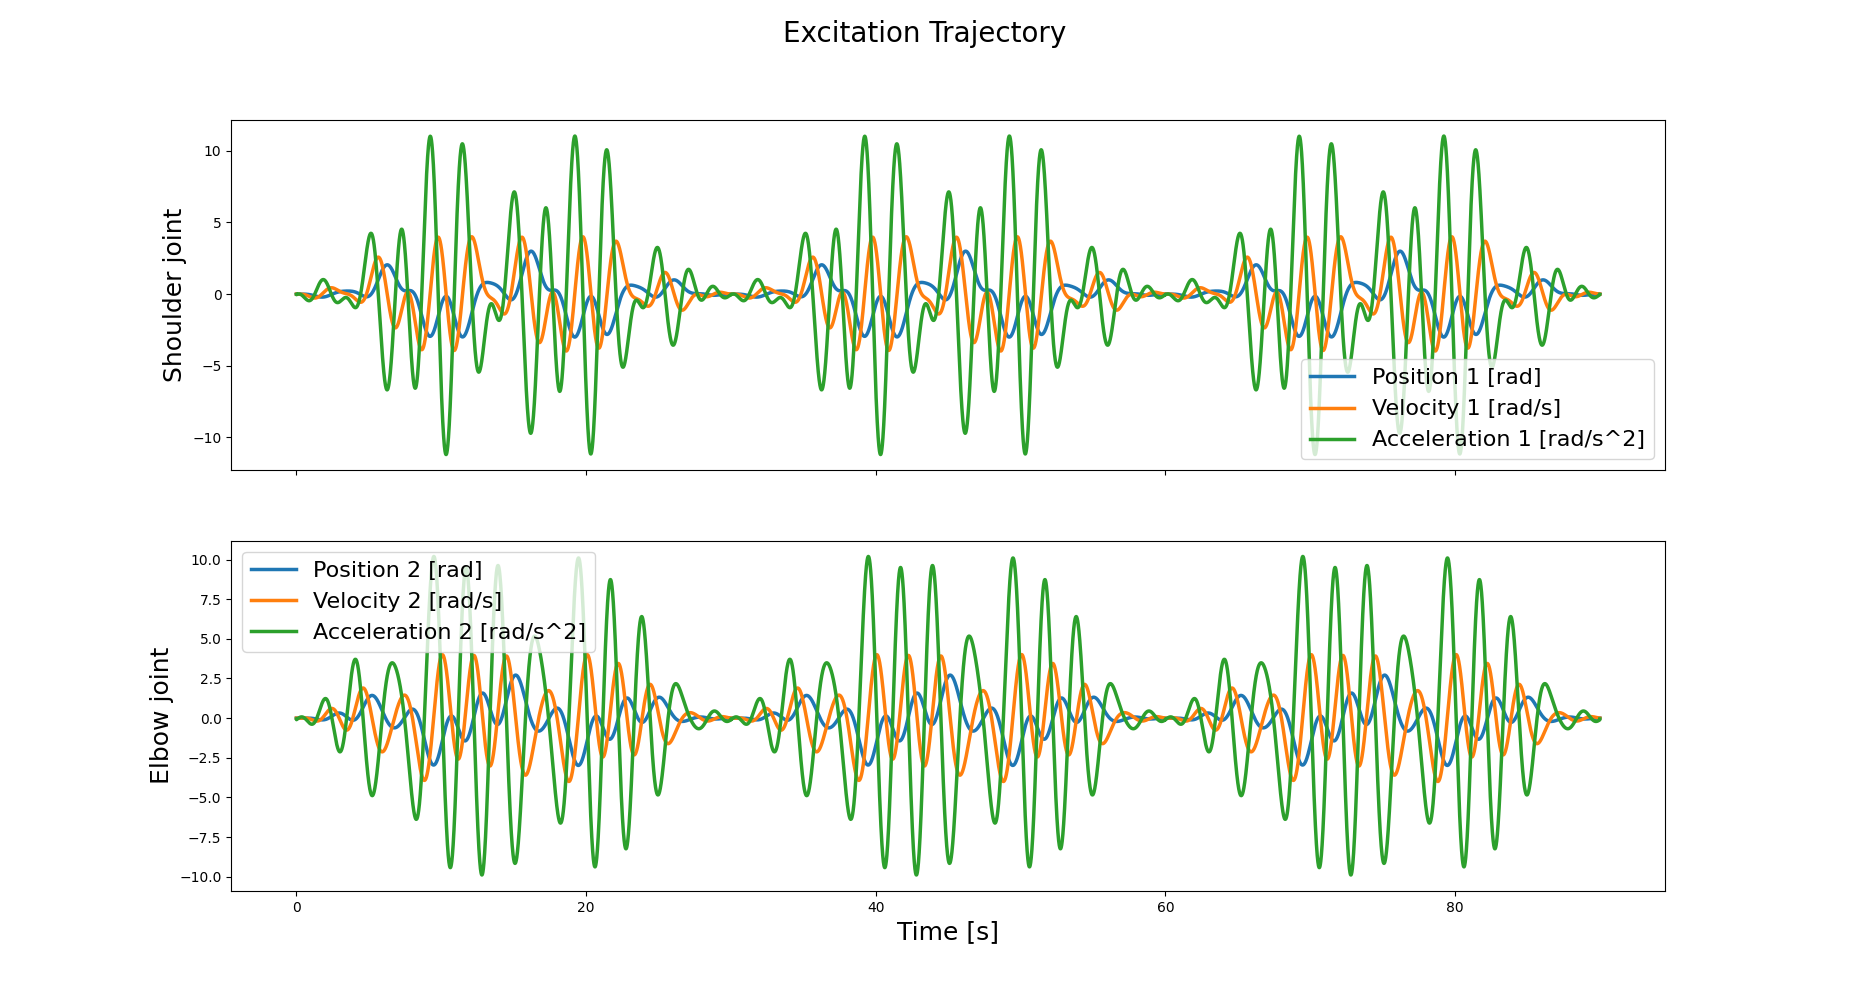
\includegraphics[width=1.1\linewidth]{figures/hardware_setup/excitation_traj.png}
    \caption{Excitation trajectory}
    \label{fig:excitation_traj}
\end{figure}

\textbf{Parameter Estimation:}

To determine the most accurate system parameters, a least squares optimization can be performed on the recorded data. The objective of the least squares optimization is to find the values of model parameters that minimize the sum of squared differences between the observed output data and the model's predictions. The objective function can be expressed as:

\begin{equation}
J(\theta) = \sum (y_{\text{observed}} - y_{\text{predicted}}(\theta))^2
\end{equation}

Where:
\begin{itemize}
\item $J(\theta)$ is the cost function to be minimized.
\item $\theta$ represents the vector of model parameters to be estimated.
\item $y_{\text{observed}}$ is the vector of observed output data.
\item $y_{\text{predicted}}(\theta)$ is the vector of model predictions based on the current parameter values $\theta$.
\end{itemize}

The optimization uses the CMA-ES (Covariance Matrix Adaptation Evolution Strategy) algorithm\cite{hansen2001completely}, and the identified model parameters are shown in Table \ref{tab:parameters}. These parameters are based on design C ($l_1 = 0.2m$, $l_2 = 0.3m$), which is used in real-world tests.

\begin{table}[H]
\centering
\begin{tabular}{|c|c|}
\hline
\textbf{Parameter} & \textbf{Value} \\
\hline
$I_1$ & 0.031887199591513114 \\
$I_2$ & 0.05086984812807257 \\
$I_r$ & 6.287203962819607e-05 \\
$b_1$ & 0.001 \\
$b_2$ & 0.001 \\
$c_{f1}$ & 0.16 \\
$c_{f2}$ & 0.12 \\
$g$ & 9.81 \\
$g_r$ & 6.0 \\
$l_1$ & 0.2 \\
$l_2$ & 0.3 \\
$m_1$ & 0.5234602302310271 \\
$m_2$ & 0.6255677234174437 \\
$r_1$ & 0.2 \\
$r_2$ & 0.25569305436052964 \\
\hline
\end{tabular}
\caption{Parameter values from system identification}
\label{tab:parameters}
\end{table}


\section{Sim-to-Real transfer}
Transferring working models from simulation to real systems to produce similar performance has always been a challenge in controller design. This challenge is even more pronounced in model-free reinforcement learning for two main reasons.

Firstly, model-free reinforcement learning relies solely on interaction with the environment to gain experience and select actions. While a simulation environment is merely a simplification of the real-world scenario, the agent in simulation might not capture all the factors, such as friction, sensor noise, or real-world dynamics, accurately. Therefore, a control policy optimized for a simplified model might not perform as expected in the more intricate real world.

Secondly, many simulations operate in discrete time and space, whereas the real world functions continuously. In our implementation, the control frequency presents a significant challenge. We use a control frequency of 100 Hz in simulation; however, it does not suffice in the real system. To enhance performance, we increased the control frequency to 400 Hz when experimenting on the real system, and this adjustment yielded positive results.

\subsection{Validation with noisy simulation environment}
In addressing the challenge of sim-to-real transfer, multiple agents were trained using the Soft Actor-Critic (SAC) algorithm under similar setups in an ideal environment. These agents were then subjected to validation within a noisy environment, which is an ideal environment incorporated with real-world features. Only those agents demonstrating robustness to perturbations within this environment were advanced to real-world tests. Agents that did not withstand the noisy environment were deemed insufficiently robust and subsequently discarded.

In the course of real world experiments, four critical factors were identified that differ from ideal simulations: friction, measurement noise, latency, and torque responsiveness.

\textbf{Friction:}

Friction, identified as the predominant factor affecting performance, was not accounted for in the simulated training environment. To bridge this gap with real-world conditions, a friction compensation strategy was employed, starting with modeling the friction based on Coulomb’s law as detailed in Equation \ref{eq:friction_function}. 

Since frictional force counteracts the relative motion between contact surfaces, this compensation involved exerting additional torque in the same direction as the angular motion, providing the system with the necessary energy to overcome the effects of friction.

Despite the friction coefficients \(c_{f1}\) and \(c_{f2}\) being ascertained during the system identification phase, they were subsequently found to be imprecise during real system testing. To refine these coefficients, free-fall tests were conducted, which entailed releasing the double pendulum from a slight angular displacement and allowing it to descend under the force of gravity. Given the coupling influence of the two links, one joint was immobilized during the friction coefficient tuning of the other: the elbow joint remained static while estimating the shoulder joint's coefficient, and vice versa. Manual adjustments to the friction coefficients were made until the position output of the tested joint resulted in a sine wave without decay.

\textbf{Measurement noise:}

Measurement noise has been identified as the second most critical factor. The position displacement is measured with high accuracy using built-in encoders in the AK80-6 motors. However, the velocity measurement, which is derived as the first derivative of the position measurement, tends to introduce a relatively higher error. In the ideal environment, measurement error for both position and velocity is assumed to be non-existent. Nonetheless, this error is considerable in real-world applications.

To tackle this problem, the measurement error has been modeled as a normal distribution, with the mean representing the true velocity value and a manually adjustable standard deviation. The measurement noise vector is denoted by \(\epsilon = [\Delta p_1, \Delta p_2, \Delta v_1, \Delta v_2]^T\), and is assumed to follow a multivariate normal distribution:
\begin{equation}
\epsilon \sim \mathcal{N}(\boldsymbol{\mu}, \boldsymbol{\Sigma})
\end{equation}
where \(\boldsymbol{\mu}\) is the vector of means, and \(\boldsymbol{\Sigma}\) is the \(4 \times 4\) covariance matrix, representing the uncertainty spread of the noise across each dimension. The measurements for the four states are presumed to be independent, rendering \(\boldsymbol{\Sigma}\) a diagonal matrix. In practice, \(\mu = 0\) and \(\Sigma = \text{diag}(0,0,0.5,0.5)\), indicating an omission of measurement noise on positions and a focus on the velocity measurement noise.

\textbf{Latency:}

Latency has been identified as the third significant factor. Given that any communication system requires time to transmit and receive data, and programs also require time to execute, latency is an inevitable aspect. Such latency presents a substantial challenge to control systems, especially those based on reinforcement learning. Reinforcement learning operates on the principles of Markov Decision Processes (MDPs), which follow the Markov property. According to this property, the future state of a MDP process is determined solely by the current state and action, and not by the sequence of states that preceded it. However, latency compromises the Markov property by inducing state mismatches and fostering dependencies on historical data. During free-fall tests, the maximum latency observed was 0.015 seconds. Therefore, this value has been established as the standard latency.

\textbf{Torque responsiveness:}

The fourth factor to be considered is torque responsiveness. In real hardware tests, it was observed that motors struggle to match the torque output with rapidly alternating control signals, particularly when there are significant differences between consecutive time steps. To model this phenomenon in noisy simulation, a discount coefficient \( c_{tr} \) is applied to the change in control signals. The actual applied torque \(u_{\text{real}}\) is the sum of the previous torque \(u_{\text{previous}}\) plus the discounted change in torque \(u_{\text{current}} - u_{\text{previous}}\). The calculation is expressed as follows:

\begin{equation}
 u_{\text{real}} = u_{\text{previous}} + c_{tr} \cdot (u_{\text{current}} - u_{\text{previous}})
\end{equation}

When \(c_{tr}\) equals zero, the torque that is exerted on the system precisely mirrors the controller's output. A lower \(c_{tr}\) value makes it more difficult to apply significant changes to the control signal. Conversely, a policy that functions effectively with a low \(c_{tr}\) value indicates better torque smoothness. This also acts as an intuitive measure of the policy's capacity to yield smooth torque outputs. In most cases, \(c_{tr}\) is set to 0.85; however, to test the controllers' boundaries, values below 0.7 are also examined.

\subsection{Noisy training based on domain randomization}
For agents that succeeded in ideal simulations yet failed in noisy simulations, domain randomization has been identified as one method to enhance robustness.

Domain randomization \cite{tobin2017domain}, a technique conceived to narrow the gap between simulation and reality, aims to enable a model to operate effectively in real-world conditions, without the need for labeled real-world training data.

Initially emerging from the computer vision domain, domain randomization involves training a model not within a single, static simulation but rather within a diverse and perturbed environment. This is achieved by incorporating random variations into the ideal simulation. Techniques commonly employed in vision-based systems include changing the colors and textures of objects, modifying the lighting conditions, adjusting object shapes and sizes, introducing random noise to sensor data, and perturbing physical properties like friction or mass.

In the application of domain randomization to robotic manipulation tasks, disturbances introduced in the noisy simulation were employed to construct a noisy training process. This process resembles the previous ideal training process, but the environments for both the trial and evaluation phases were substituted with noisy environments. The training was warm-started with pretrained agents that had demonstrated success in ideal simulations yet performed poorly in noisy simulations.

The results of domain randomization in noisy training proved to be highly variable. Some agents significantly improved after a mere 5e6 iterations of noisy training, while others remained unchanged or worsened, with some even regressing to the point of failure in ideal simulations where they had once succeeded.


\section{Results on real hardware}
In this section, the results from the real hardware phase are presented. The content is divided into three parts. The first part discusses the procedure for selecting agents suitable for real-world testing. The second part displays the successful outcomes from an agent trained for the pendubot setup. The range of results is restricted to the pendubot setup due to the introduction of speed and position limits, which have significantly narrowed the range of possible policies. The third part discusses an unsuccessful agent in the acrobot setup. It passed ideal and noisy validations but cannot be transferred to real-world tests due to a violation of the \(2\pi\) position limit.

\begin{figure}[H]
    \centering
    \includegraphics[width=0.45\textwidth]{figures/double_pendulum_real_system.png}
    \caption{Double pendulum in real system}
    \label{fig:double_pendulum_real_system}
\end{figure}

\subsection{Agent selection procedure for real world tests}
An agent deemed suitable for real-system tests must undergo a process that includes training and validation in ideal environment, followed by validation in noisy environment. If the agent proves successful in noisy validation, it can proceed to further testing on the real system. If it does not succeed, we employ the domain randomization method in an attempt to enhance its performance. Should the retrained agent pass the noisy validation, it will then advance to real-system testing. Otherwise, it will be discarded.

\begin{figure}[H]
    \centering
    
\includegraphics[width=0.9\textwidth]{figures/hardware_result/agent_selection_procedure.png}% Second image
    \caption{Agent selection procedure for real hardware tests}
    \label{fig:agent_selection}
\end{figure}

\subsection{Pendubot results in real world}
All real hardware experiments are based on design C \( (l_1 = 0.2, l_2 = 0.3) \). For the pendubot setup, obtaining a working agent is relatively straightforward. Slight modifications were made to the training process for the ideal simulation phase by deactivating the scaling mechanism mentioned in Section 4.1 and adding a termination condition that ends the training episode if the shoulder or elbow joint exceeds \( 2\pi \), which means the agents are trained on unnormalized real physical state values with strict constraints on speed and velocity boundaries. Utilizing the parameters listed in Table~\ref{tab:training_parameters_real_world_pendubot}, the training process successfully yielded a working model in the ideal simulation within \( 2 \times 10^7 \) timesteps.

\begin{table}[H]
  \centering
  \begin{tabular}{p{2cm} | p{3cm} | p{3cm} | p{3cm}}
  Robot & Quadratic Reward  & Constant Reward & LQR\\
  \hline
  \multirow{5}{*}{Pendubot} & \(Q_1\) = 100 &  & \(Q_1\) = 0.97\\
  & \(Q_2\) = 100  & \(r_{line}=1e3\) & \(Q_2\) = 0.93\\
  & \(Q_3\) = 1.0  & \(r_{vel}=0.0\) & \(Q_3\) = 0.39\\
  & \(Q_4\) = 1.0  & \(r_{LQR}=1e5\)& \(Q_4\) = 0.26\\
  & \(R\) = 1e-2  & & \(R\) = 0.11\\
  \end{tabular}
 \caption{Hyper parameters used for training pendubot agents for real world tests}
 \label{tab:training_parameters_real_world_pendubot}
\end{table}

\begin{figure}[H]
    \centering
    \begin{subfigure}[b]{0.47\textwidth}
        \centering
        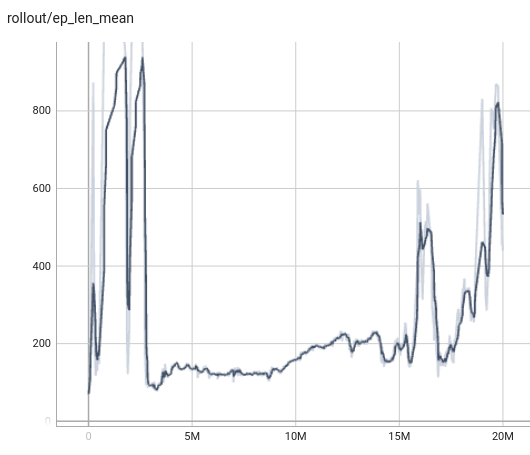
\includegraphics[width=\textwidth]{figures/hardware_result/train_without_limit_ep_length.png}
        \caption{Mean episode length}
        \label{fig:mean episode length}
    \end{subfigure}
    \hfill % add some horizontal spacing
    \begin{subfigure}[b]{0.47\textwidth}
        \centering
        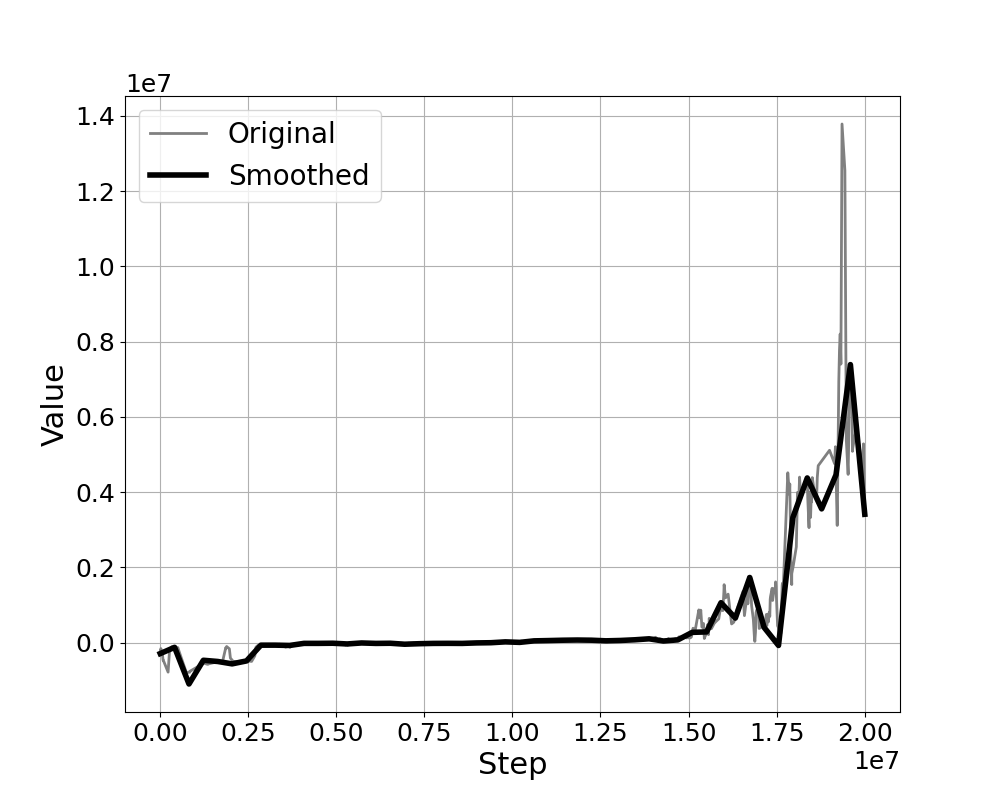
\includegraphics[width=\textwidth]{figures/hardware_result/train_without_limit_ep_reward.png}
        \caption{Mean episode reward}
        \label{fig:mean episode reward}
    \end{subfigure}
    \caption{Training curves of the working agent on pendubot}
    \label{fig:training_curves_for_real_world}
\end{figure}

Figure \ref{fig:training_curves_for_real_world} presents the training curve for the acquisition of an agent designated for real-world pendubot experiments, utilizing an ideal training process. As depicted in Figure \ref{fig:mean episode length}, the mean episode length initially approaches the maximum of 1000, but then it rapidly descends to below 200 after 3e6 training steps. This descent indicates that the agent consistently attempts to rotate beyond 360 degrees in pursuit of higher rewards. A sign of emergence from this performance valley is observed at 15e6 training steps, with a subsequent significant increase in episode length. Correspondingly, the mean episode reward, as illustrated in Figure \ref{fig:mean episode reward}, also shows a gradual increase before 15e6 time steps, followed by a rapid ascent thereafter.

The agent is put to the test in an ideal environment for validation. The results are 100\% successful, as shown in Figure \ref{fig:pendubot_ideal_working}. The switching time between the SAC controller and the LQR controller occurs in less than 1 second. After taking over, the LQR controller is able to maintain balance around the goal state until the end of the experiment.

\begin{figure}[H]
    \centering
    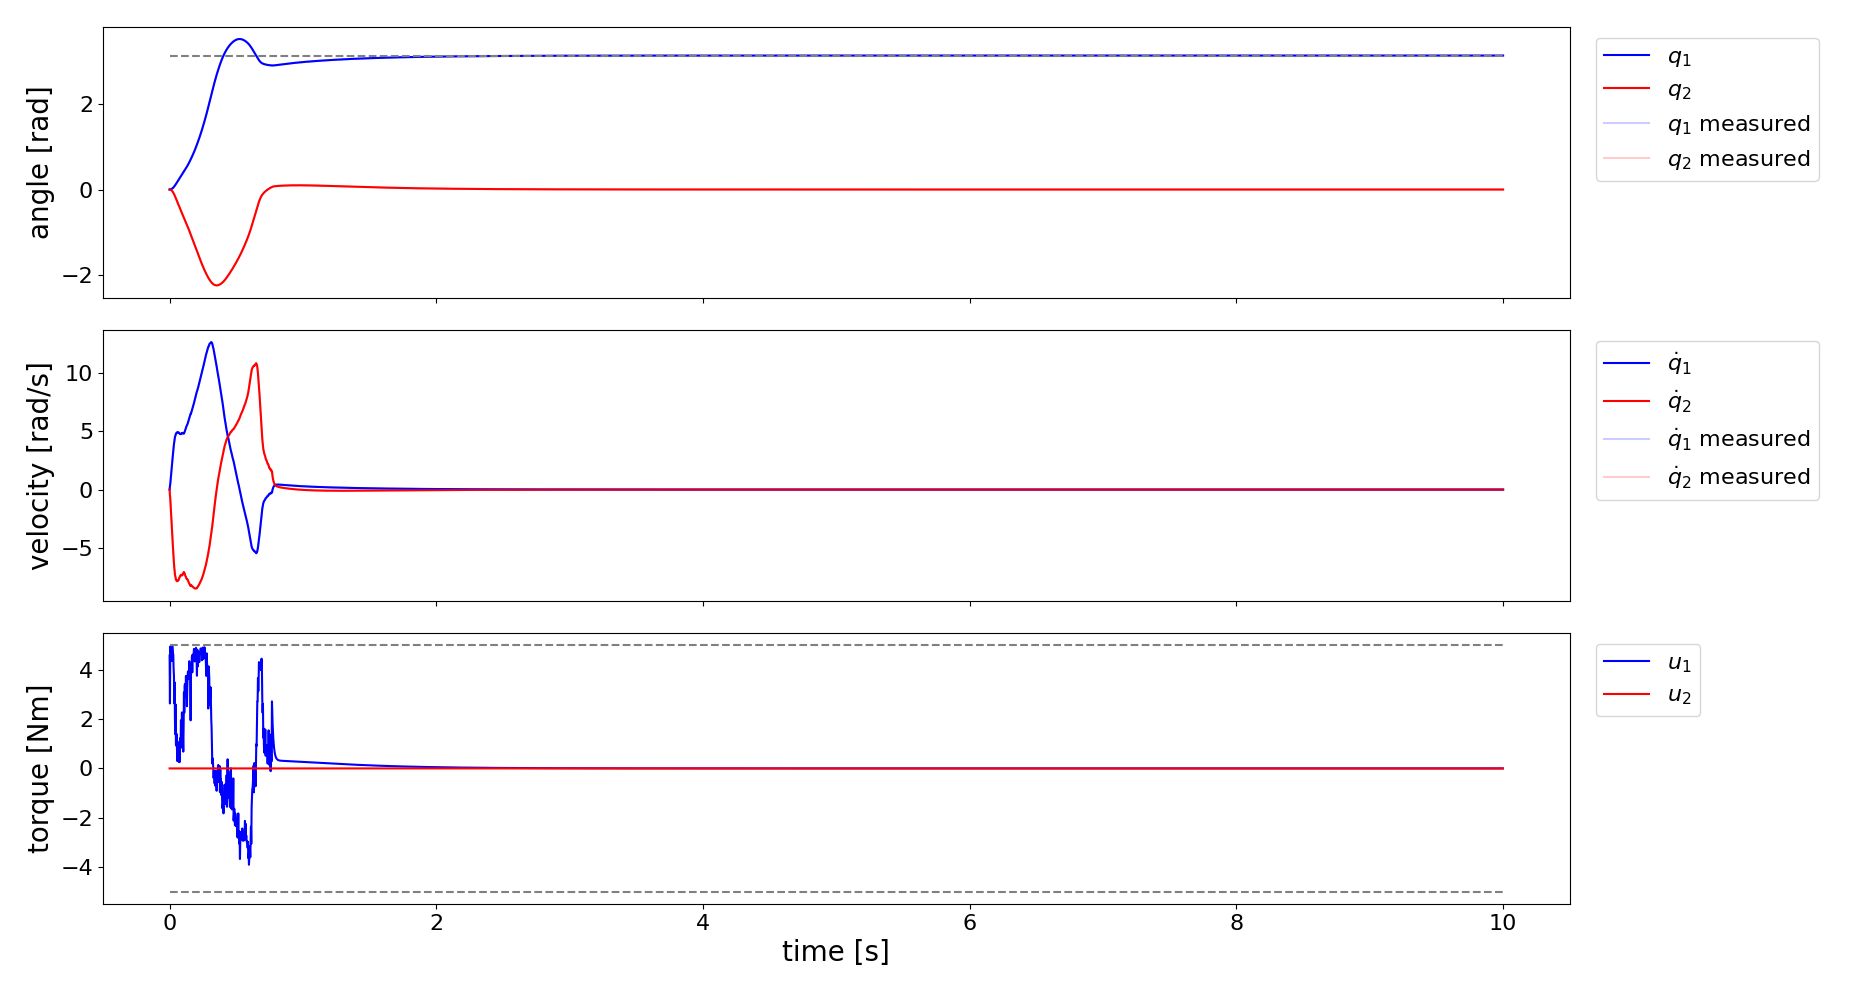
\includegraphics[width=0.95\linewidth]{figures/hardware_result/pendubot_ideal_validation_designC.1.png}
    \caption{Pendubot result in the ideal environment}
    \label{fig:pendubot_ideal_working}
\end{figure}

\begin{figure}[H]
    \centering
    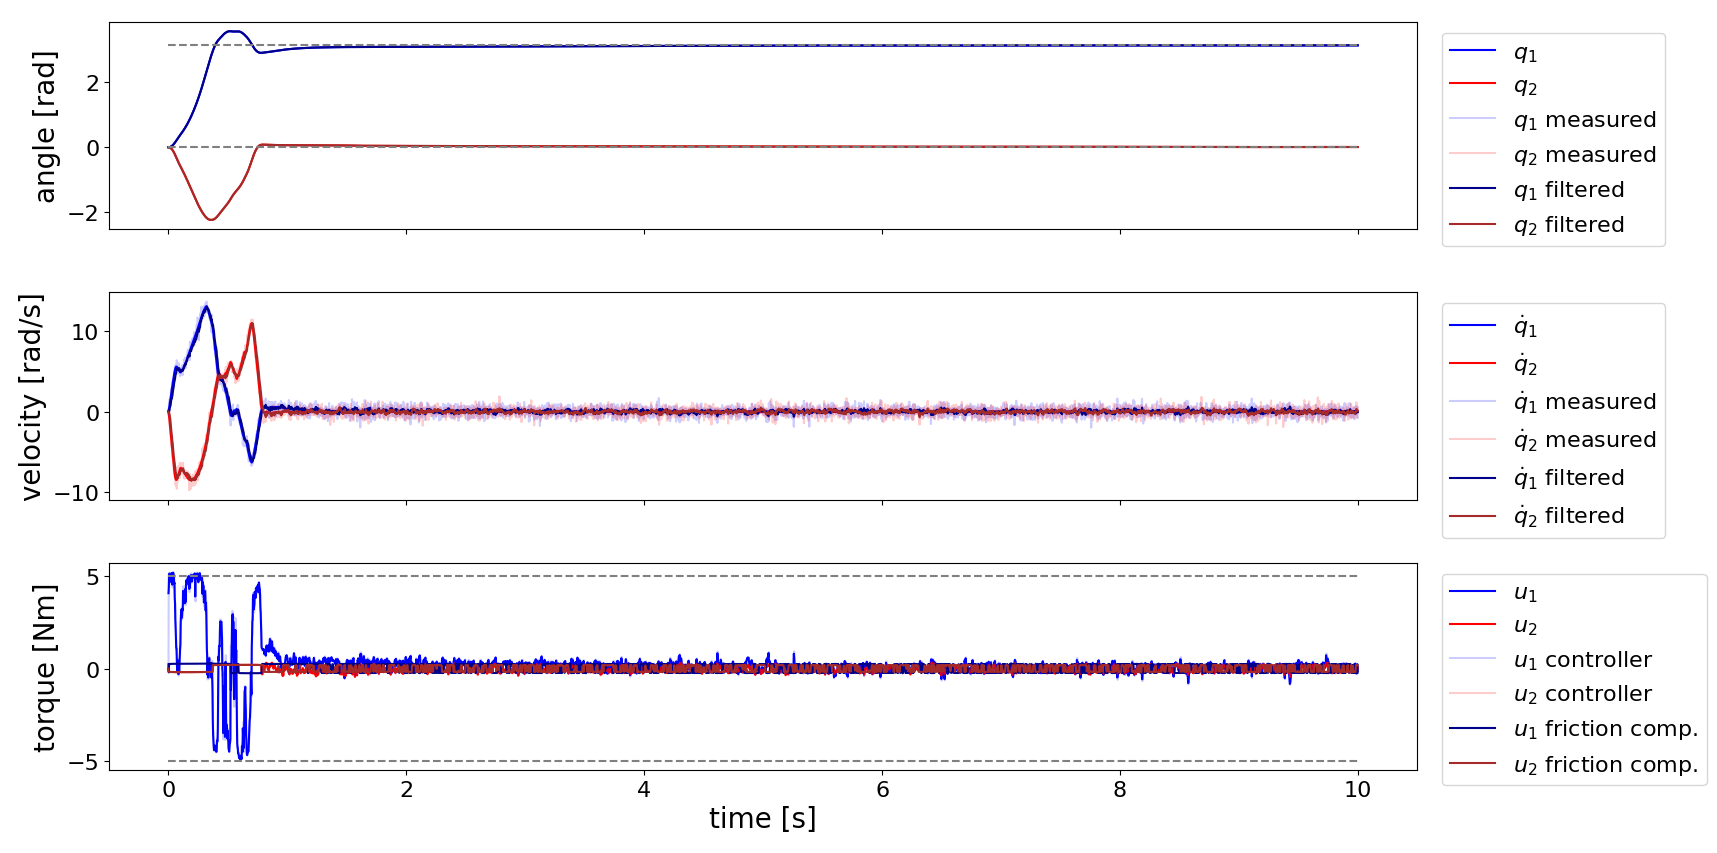
\includegraphics[width=1.0\linewidth]{figures/hardware_result/pendubot_noisy_simulation_designC.1.png}
    \caption{Pendubot result in the noisy environment}
    \label{fig:pendubot_noisy_working}
\end{figure}

Subsequently, the agent was subjected to noisy validation. In a noisy simulation, the pretrained agent was found to succeed at rate of 40\%, as demonstrated in Figure \ref{fig:pendubot_noisy_working}. In successful trials, the transition time between the SAC controller and the LQR controller occurred around 1 second. The LQR controller was still very effective in maintaining the system's stability. In unsuccessful trials, two scenarios occurred. Most often, the transition did not occur, and the system, remaining under the influence of the SAC controller, was inadequate for maintaining stability. In a few cases, although the transition did occur, the LQR controller failed to maintain the system's relative stable state around the upright position, resulting in experimental failure.

Though the noisy validation only have 40\% success rate, we consider the above shown agent ready for a real-world test, so we deploy it onto the test bench for the real world evaluation. A control frequency of 400Hz was utilized. The agent's average success rate in the real system was 40\%, aligning with the success rate observed during noisy validation. A depiction of one such successful outcome is presented in Figure \ref{fig:pendubot_real_working}. 

\begin{figure}[H]
    \centering
    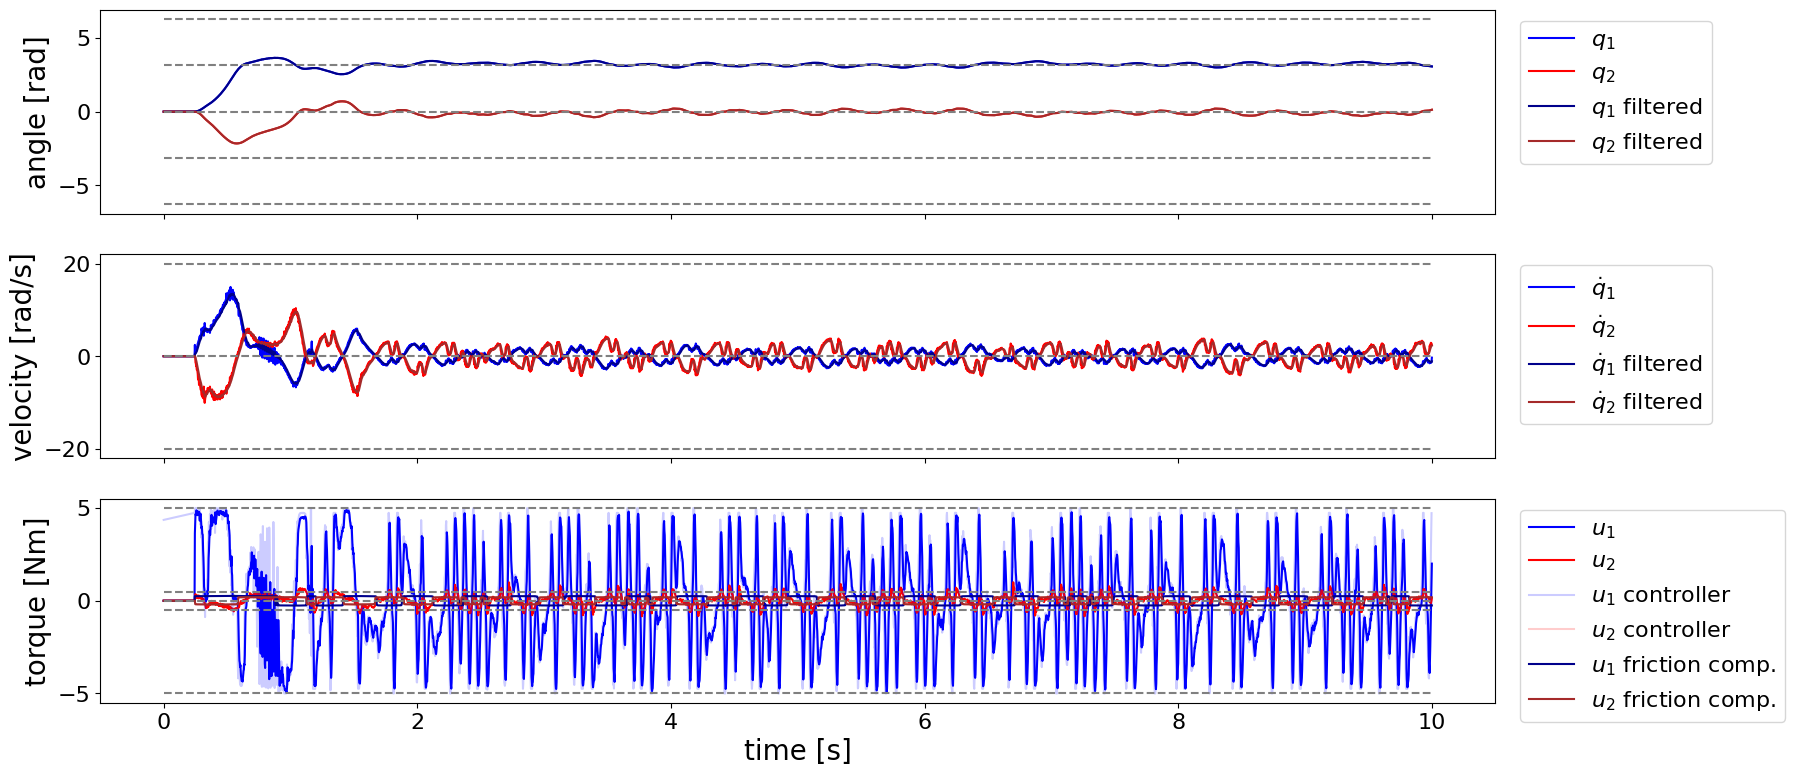
\includegraphics[width=1.0\linewidth]{figures/hardware_result/pendubot_real_system_working.png}
    \caption{Result of a successful pendubot experiment on real system}
    \label{fig:pendubot_real_working}
\end{figure}

The transition to the LQR controller occurred smoothly at approximately one second. Upon assuming control, the LQR controller succeeded in sustaining the system's upright position, albeit with vibrations, until the completion of the experiment. Contrary to the results in both noisy and ideal simulations, the torque applied by the LQR controller was noticeably less smooth, resulting in greater amplitude of position and velocity vibrations. Given that the feature of self-stabilization had been evident during the ideal validation phase, an attempt was made to omit the LQR controller, allowing the agent to execute the swing-up and stabilize independently; however, this approach proved unsuccessful.

In unsuccessful trials, similar problems that occurred during noisy validation recurred. The system either failed to switch from the SAC controller to the LQR controller, or the LQR controller was unable to maintain stability. The latter scenario is more likely to occur in real-world tests than in noisy validation.


\subsection{Acrobot results in real world}
Training for the acrobot setup has encountered numerous challenges, which can be summarized into the following aspects:

\textbf{Violation of Speed and Position Limit:}

The introduction of new rules, with a speed limit set at 20 rad/s and a position limit set at \(2\pi\), has made it more challenging to train a functional agent in the acrobot setup. Attempts have been made to train agents using unscaled real physical state values with a termination condition aimed at keeping the agent within the position limit; however, this approach did not perform as well as it did with the pendubot setup. Despite the application of 5e7 timesteps (which takes approximately 5 hours), neither the mean episode length nor the mean episode reward exhibited growth. A return to the method of training based on scaled state values without termination conditions eventually yielded a working model in ideal validation, although the \(2\pi\) position limit was violated.

\textbf{Inconsistency in Training:}

The training of acrobot agents has proven to be highly unstable. Despite the use of consistent and carefully tuned hyperparameters, training success has varied. There are instances when significant growth in mean episode reward suggests that training is progressing correctly, yet the resulting agent may perform inconsistently in ideal simulations.

\textbf{Long Training Hours:}

When compared to pendubot training, exploration in the acrobot setup often requires more time. While pendubot training typically produces a functional agent within 2e7 timesteps, acrobot training may take between 3e7 to 4e7 timesteps, with no guarantee that the resulting agent will pass an ideal validation. Such iterations, taking 3-4 hours each, are considerably time-consuming.

The most favorable outcome in the acrobot setup has been an agent that functions effectively in both ideal and noisy validations. It was trained using parameters detailed in Table \ref{tab:training_parameters_real_world_acrobot}, with an active scaling mechanism and in the absence of termination conditions, indicating that the agent was trained using normalized state values.

\begin{table}[H]
  \centering
  \begin{tabular}{p{2cm} | p{3cm} | p{3cm} | p{3cm}}
  Robot & Quadratic Reward  & Constant Reward & LQR\\
  \hline
  \multirow{5}{*}{Pendubot} & \(Q_1\) = 100 &  & \(Q_1\) = 1.92\\
  & \(Q_2\) = 90  & \(r_{line}=1e3\) & \(Q_2\) = 1.92\\
  & \(Q_3\) = 1.0  & \(r_{vel}=1e4\) & \(Q_3\) = 0.3\\
  & \(Q_4\) = 1.0  & \(r_{LQR}=1e5\)& \(Q_4\) = 0.3\\
  & \(R\) = 1e-2  & & \(R\) = 0.82\\
  \end{tabular}
 \caption{Hyper parameters used for training acrobot agents for real world tests}
 \label{tab:training_parameters_real_world_acrobot}
\end{table}

As shown in Figure \ref{fig:acrobot_training_curve}, the reward for this agent experienced a smooth increase up to 2.5e7 timesteps and then a rapid ascent in the final 5 million timesteps. Because a termination condition was not implemented, the episode length remained consistently at 1000. This outcome was anticipated and led to  a working agent in an ideal environment.

\begin{figure}[H]
    \centering
    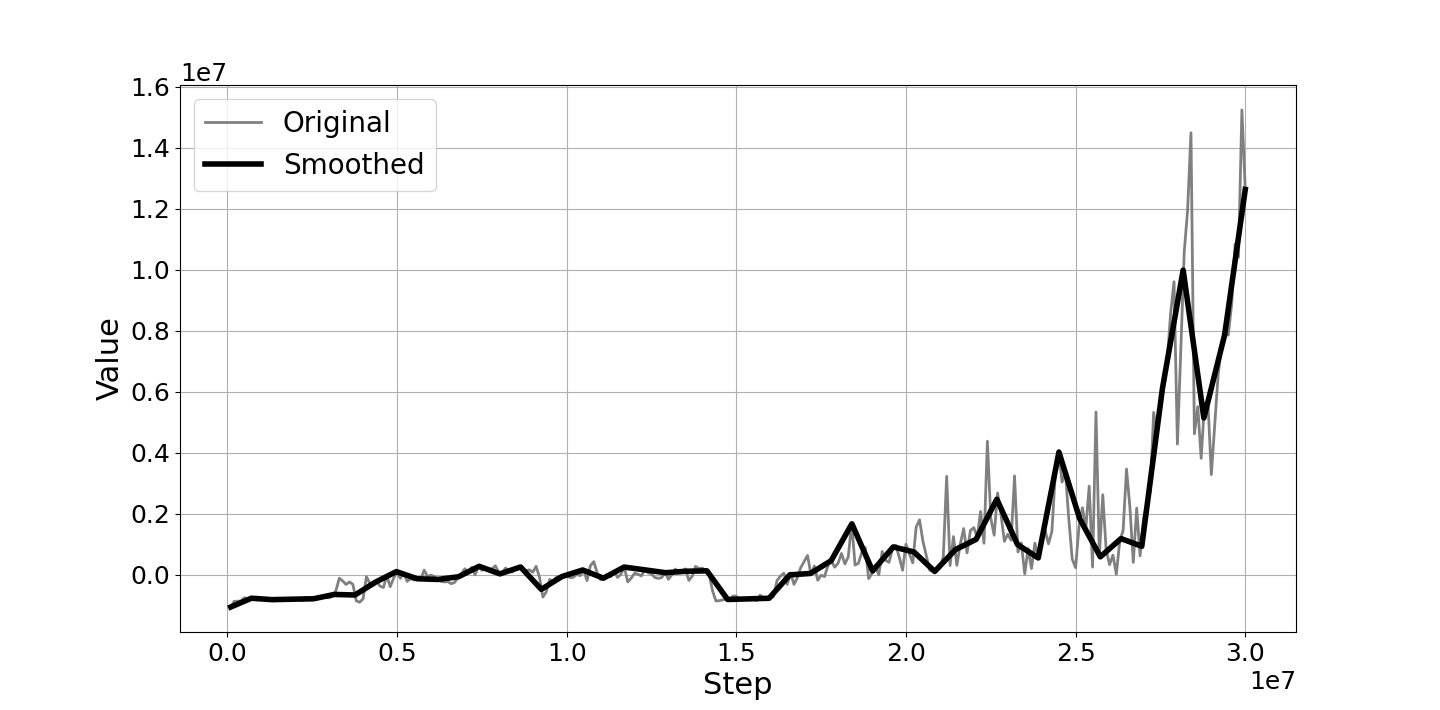
\includegraphics[width=1.0\linewidth]{figures/hardware_result/acrobot_learning_curve_real_world.png}
    \caption{Training curve of best result in acrobot setup}
    \label{fig:acrobot_training_curve}
\end{figure}

The behavior of this agent during ideal validation is shown in Figure \ref{fig:acrobot_ideal}. The swing-up is performed by the SAC controller within 2 seconds. After the LQR controller takes over, the system maintains stability around the highest position for a prolonged period. The ideal validation is considered successful.

\begin{figure}[H]
    \centering
    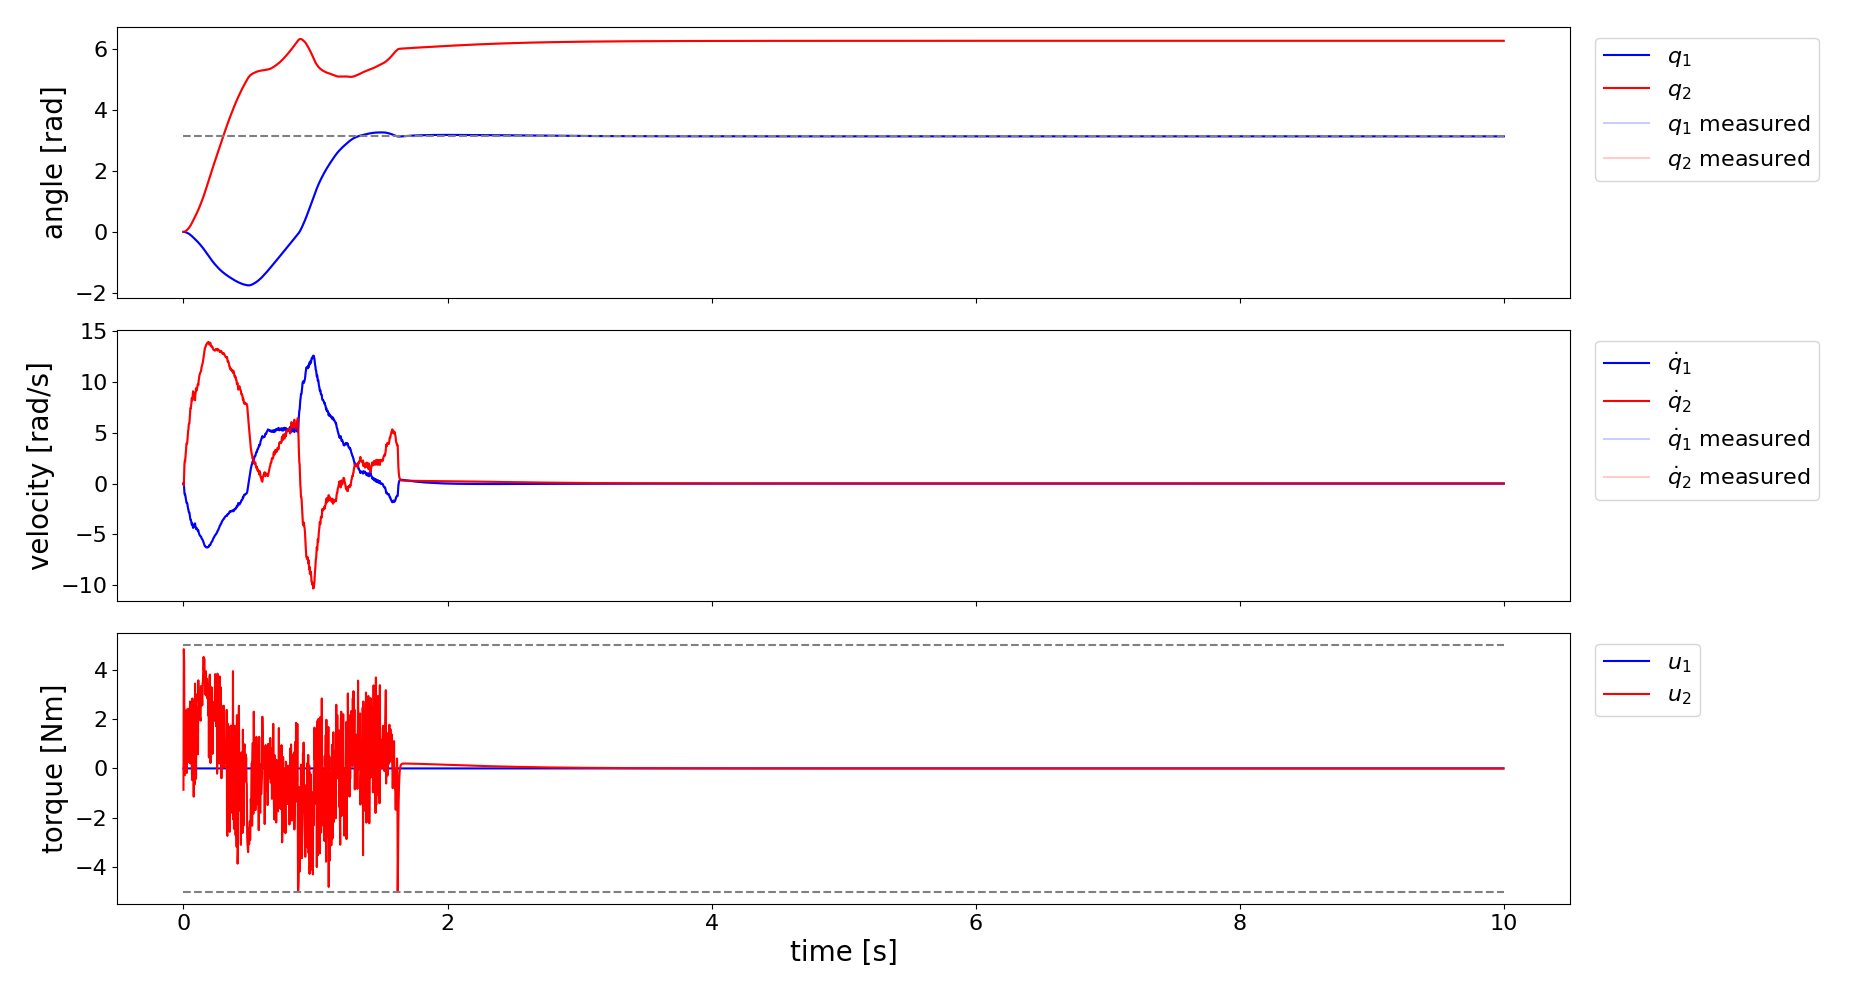
\includegraphics[width=0.95\linewidth]{figures/hardware_result/acrobot_ideal_simulation_designC.1.png}
    \caption{Acrobot result in ideal environment}
    \label{fig:acrobot_ideal}
\end{figure}

The agent operates successfully within a noisy simulation after ideal validation, eliminating the need for further noisy training. The success rate is approximately 50\%. Figure \ref{fig:acrobot_noisy} shows one of the successful tests.

In successful trials, the swing-up phase conducted by the SAC controller concludes within 2 seconds. Although the torque applied in ideal environment tests is already quite noisy, the torque in a noisy environment exhibits even greater fluctuations. Once the LQR controller takes effect, the system stabilizes around the goal state until the experiment concludes. In unsuccessful trials, the inability to switch to the LQR controller is the primary issue. But the agent has high recovery ability, the system sometimes misses the first transition oppotunity and making several rotations before it finds itself reaching a point for LQR controller to take over.

\begin{figure}[H]
    \centering
    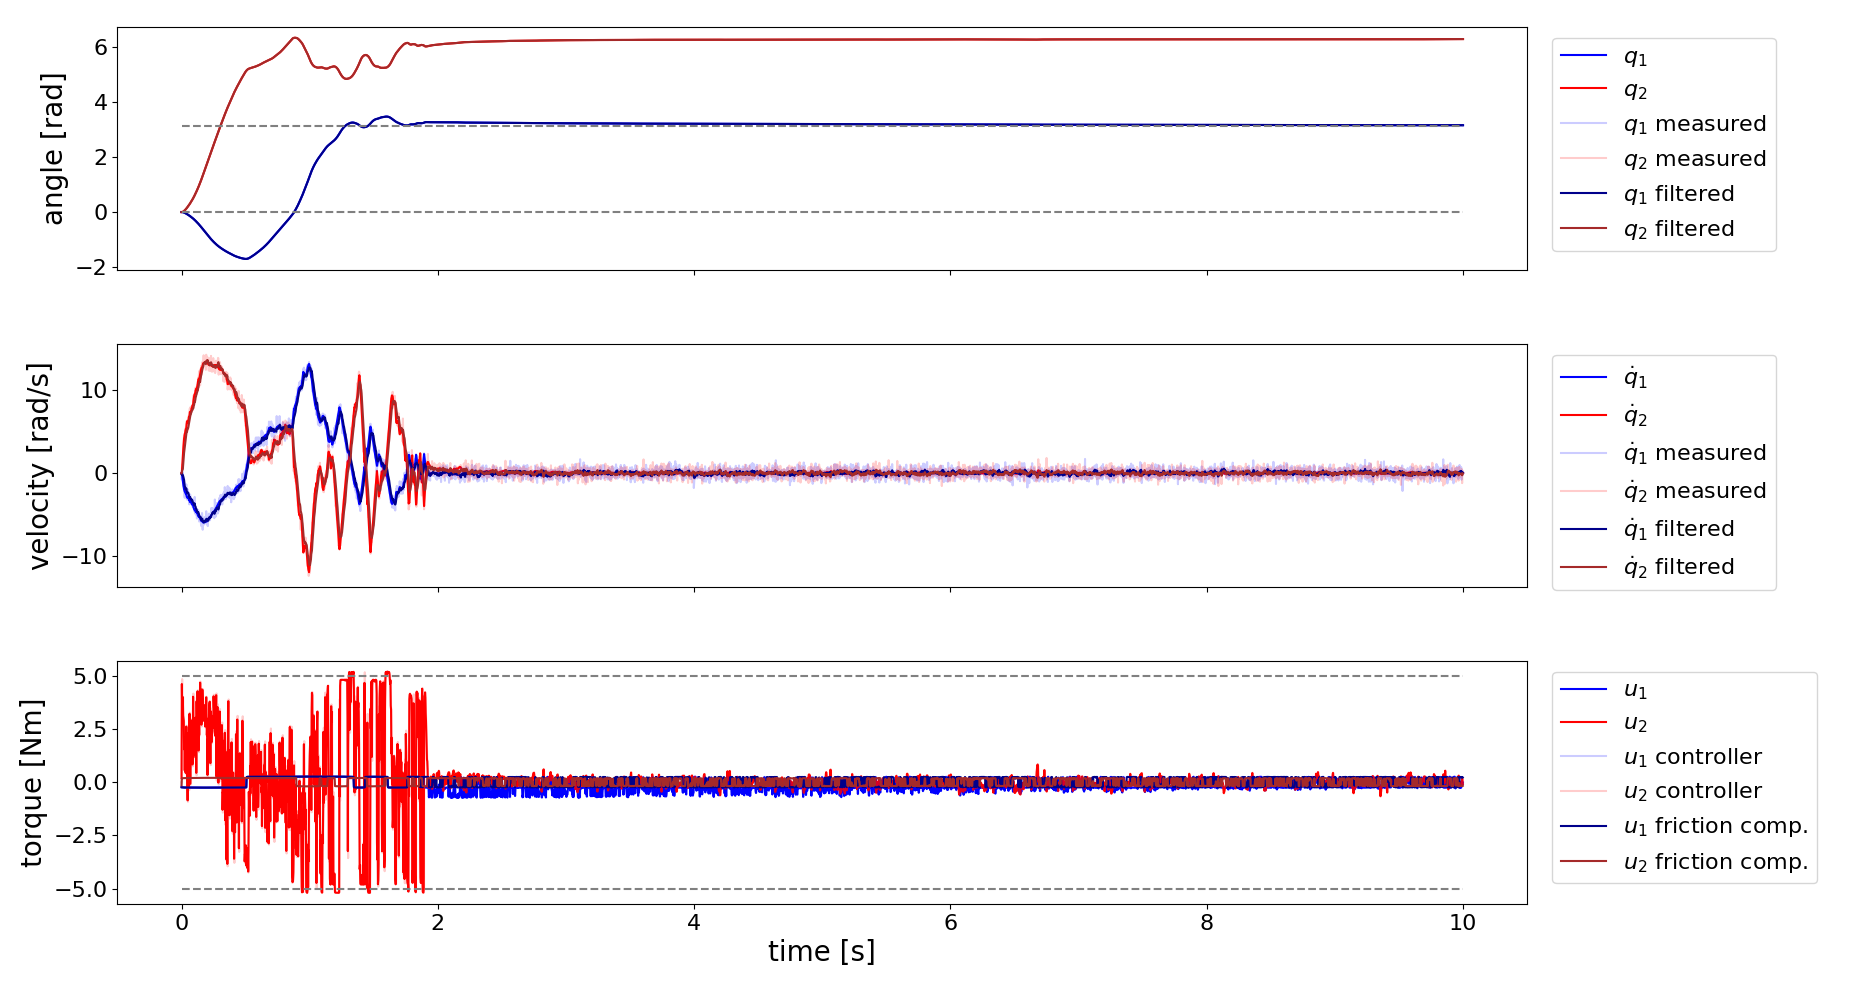
\includegraphics[width=1.0\linewidth]{figures/hardware_result/acrobot_noisy_simulation_designC.1.png}
    \caption{Acrobot result in noisy environment}
    \label{fig:acrobot_noisy}
\end{figure}

Due to the agent's violation of the \(2\pi\) position limit, it has been deemed unsuitable for real-world tests. Consequently, no additional results from real-world tests in the acrobot setup are presented.

\cleardoublepage

\chapter{Discussion and Conclusion}
In this chapter, we delve into the results of experiments conducted in both simulation and on the real system. The chapter is structured as follows: The first section discusses the three facets of leaderboard analysis, namely simulation, robustness, and real hardware, respectively. The second section summarizes our current findings and draws conclusions from the project.

\section{Discussion}
\subsection{Interpretation of simulation leaderboard}
In Table \ref{tab:performance_ideal}, the performance leaderboard results for both the pendubot and acrobot in simulation experiments are presented. Three types of controllers are listed for comparison, namely model-free reinforcement learning(MFRL) based controller, model-based reinforcement learning(MBRL) based controller and trajectory based controller.

The SAC+LQR controller is our design and is a representative of model-free reinforcement learning method. 

MC-PILCO~\cite{amadio2022model}, which stands for Monte Carlo Probabilistic Inference for Learning Control, is a model-based reinforcement learning method. It utilizes probabilistic models to predict the system's dynamics and employs Monte Carlo methods to optimize control policies based on these predictions. This method was implemented by a team from the University of Padova~\cite{Libera2023AthleticIO}. 

tvLQR is an extension of the standard Linear Quadratic Regulator (LQR) control design. It is a trajoctory based control method, tailored for systems with time-dependent state-space matrices or where the optimal control needs to be dynamic. Representing the optimal control method, it was implemented by a separate team from DFKI RIC\cite{2023_ram_wiebe_double_pendulum}.

\begin{table}[H]
  \centering
 \begin{tabular}{lcccccc}
 \hline
 Criteria & \multicolumn{2}{c}{SAC+LQR} & \multicolumn{2}{c}{MC-PILCO} & \multicolumn{2}{c}{tvLQR} \\
 & Pendubot & Acrobot & Pendubot & Acrobot & Pendubot & Acrobot \\
 \hline
 Swingup Success & success & success & success & success & success & success \\
 Swingup time [s] & \textbf{0.65} & 2.06 & 1.43 & \textbf{1.1} & 4.2 & 3.98 \\
 Energy [J] & 9.4 & 29.24 & 12.67 & \textbf{9.81} & \textbf{9.06} & 10.92 \\
 Max. Torque [Nm] & 5.0 & 5.0 & \textbf{2.4} & \textbf{2.82} & 2.82 & 5.0 \\
 Integrated Torque [Nm] & \textbf{2.21} & 4.57 & 3.48 & \textbf{1.27} & 2.57 & 2.27 \\
 Torque Cost [N²m²] & 8.58 & 12.32 & 7.77 & \textbf{2.27} & \textbf{2.0} & 2.47 \\
 Torque Smoothness [Nm] & 0.172 & 0.954 & 0.07 & \textbf{0.057} & \textbf{0.031} & 0.077 \\
 Velocity Cost [m²/s²] & \textbf{44.98} & 193.78 & 94.68 & 242.44 & 137.31 & \textbf{100.34} \\
 RealAI Score & 0.801 & 0.722 & \textbf{0.891} & \textbf{0.869} & 0.827 & 0.8 \\
 \hline
 \end{tabular}
 \caption{Performance scores of various controllers for pendubot and acrobot experiments.}
 \label{tab:performance_ideal}
\end{table}

All three controllers are successful with both the Pendubot and Acrobot setups.

In the Pendubot setup, the performance of the SAC+LQR controller is commendable, particularly with a swift swing-up time of 0.65s. The energy consumption of the SAC+LQR controller (9.4J) is significantly lower than that of the MC-PILCO controller (12.67J) and is nearly on par with the tvLQR controller (9.06J). The integrated torque of SAC+LQR controller is also the lowest. Additionally, its overall RealAI score is competitive, closely trailing the scores of MC-PILCO and tvLQR. However, a notable drawback is its torque smoothness; it performs the worst among the three controllers, being 2.46 times that of MC-PILCO and 5.55 times that of tvLQR.

For the Acrobot setup, the SAC+LQR controller loses its edge in both swing-up time and energy consumption. Its deficit in torque smoothness becomes even more pronounced, leading to a considerably lower RealAI score compared to the other two controllers.

In general, the SAC+LQR controller demonstrates competitive performance in simpler tasks, such as the pendubot, especially excelling in swing-up time. However, when faced with a more complex challenge like the Acrobot, its performance declines. The MC-PILCO consistently delivers the best overall performance across both setups and is notable for its remarkably low maximum torque input and consistent torque smoothness. Conversely, the tvLQR, a trajectory based method, highlights its effectiveness in both scenarios. While its swing-up time is relatively extended, its energy consumption and torque smoothness are commendably low, leading to a moderate RealAI score.

\subsection{Interpretation of robust leaderboard}
The results of robustness leaderboard is shown in Table \ref{tab:robustness}. In comparison, the SAC+LQR controller achieves a moderate overall robustness score among the three controllers. It exhibits a higher resistance to model inaccuracy (71.9\% for pendubot and 76.7\% for acrobot) compared to MC-PILCO (45.2\% for pendubot and 40.5\% for acrobot) and tvLQR (75.2\% for pendubot and 59.0\% for acrobot). While the other two controllers demonstrate a noticeable decline when tackling the more complex acrobot task, the performance of the SAC+LQR remains consistent. Additionally, SAC+LQR offers better resistance against velocity measurement noise compared to MC-PILCO, though the top score in this category is held by tvLQR. Apart from MC-PILCO, the other two controllers display consistent and strong robustness regarding torque noise and torque response. When considering time delay, tvLQR outperforms both SAC+LQR and MC-PILCO owing to its nature as a trajectory-based controller, which is less affected by the Markov decision process.

\begin{table}[H]
  \centering
 \begin{tabular}{lcccccc}
 \hline
 Criteria & \multicolumn{2}{c}{SAC+LQR} & \multicolumn{2}{c}{MC-PILCO} & \multicolumn{2}{c}{tvLQR} \\
 & Pendubot & Acrobot & Pendubot & Acrobot & Pendubot & Acrobot \\
 \hline
 Model inaccuracy [\%] & 71.9 & \textbf{76.7} & 45.2 & 40.5 & \textbf{75.2} & 59.0 \\
 Velocity noise [\%] & \textbf{100.0} & 71.4 & 90.5 & 66.7 & \textbf{100.0} & \textbf{95.2} \\
 Torque noise [\%] & 100.0 & 100.0 & 100.0 & 81.0 & 100.0 & 100.0 \\
 Torque response [\%] & 100.0 & 100.0 & 100.0 & 90.5 & 100.0 & 100.0 \\
 Time delay [\%] & 76.2 & 61.9 & 90.5 & 19.0 & \textbf{100.0} & \textbf{76.2} \\
 Overall Score & 0.896 & 0.820 & 0.852 & 0.595 & \textbf{0.950} & \textbf{0.861} \\
 \hline
 \end{tabular}
 \caption{Robustness scores of various controllers for pendubot and acrobot experiments.}
 \label{tab:robustness}
\end{table}

In general, tvLQR achieves the best robustness scores for both pendubot and acrobot setups, followed by SAC+LQR, with MC-PILCO ranking last. While SAC+LQR boasts consistency in robustness across both setups, time delay remains a significant issue, limiting the robustness of RL-based methods.

\subsection{Interpretation of real system leaderboard}
The results of real system performance leaderboard is presented in Table \ref{tab:performance_real}. For the pendubot, SAC+LQR achieved a swing-up success rate of 40\%, while MC-PILCO had a perfect score of 100\%, and tvLQR scored 80\%. For the acrobot, SAC+LQR did not achieve success, MC-PILCO again scored 100\%, and tvLQR achieved full success as well. The swing-up time was fastest with SAC+LQR for the pendubot at 0.67 seconds, and for the acrobot, MC-PILCO had the fastest time at 1.55 seconds.

\begin{table}[H]
  \centering
 \begin{tabular}{lcccccc}
 \hline
 Criteria & \multicolumn{2}{c}{SAC+LQR} & \multicolumn{2}{c}{MC-PILCO} & \multicolumn{2}{c}{tvLQR} \\
 & Pendubot & Acrobot & Pendubot & Acrobot & Pendubot & Acrobot \\
 \hline
 Swingup Success & 4/10 & 0/10 & 10/10 & 10/10 & 8/10 & 10/10 \\
 Swingup time [s] & \textbf{0.67} & - & 1.37 & \textbf{1.55} & 4.12 & 4.03 \\
 Energy [J] & 37.12 & - & \textbf{11.66} & 17.95 & 34.02 & \textbf{13.75} \\
 Max. Torque [Nm] & 5.0 & - & \textbf{4.99} & 5.0 & 5.0 & \textbf{2.98} \\
 Integrated Torque [Nm] & 24.87 & - & \textbf{3.72} & 5.93 & 19.06 & \textbf{5.61} \\
 Torque Cost [N²m²] & 78.7 & - & \textbf{8.93} & 11.73 & 51.88 & \textbf{3.26} \\
 Torque Smoothness [Nm] & 0.774 & - & \textbf{0.54} & 0.671 & 0.643 & \textbf{0.108} \\
 Velocity Cost [m²/s²] & 114.04 & - & \textbf{84.61} & 118.38 & 242.34 & \textbf{109.77} \\
 Best RealAI Score & 0.767 & - & \textbf{0.843} & 0.82 & 0.695 & \textbf{0.822} \\
 Average RealAI Score & 0.298 & - & \textbf{0.839} & 0.817 & 0.547 & \textbf{0.821} \\
 \hline
 \end{tabular}
 \caption{Real hardware performance scores of multiple controllers for pendubot and acrobot experiments.}
 \label{tab:performance_real}
\end{table}

Apart from the swing-up time, MC-PILCO demonstrates superior performance on the pendubot, while tvLQR has the advantage for the acrobot. MC-PILCO's energy consumption on the pendubot is markedly lower, with marginally better maximum torque and a significant lead in integrated torque and torque cost metrics. The velocity cost further showcases MC-PILCO's high efficiency, contributing to its leading average RealAI score of 0.839.

In the acrobot trials, the scores are close between MC-PILCO and tvLQR. However, tvLQR outperformed MC-PILCO in terms of energy consumption and most torque-related criteria by a substantial margin. Additionally, tvLQR's torque smoothness is notably superior to that of MC-PILCO. tvLQR also achieved the highest average RealAI score of 0.821 for the acrobot.

In summary, while MC-PILCO displayed high efficiency and success rates for the pendubot, tvLQR excelled in torque smoothness and energy efficiency, particularly for the acrobot system. The SAC+LQR approach demonstrated rapid swing-up times for the pendubot but failed to register success for the acrobot.

\section{Conclusion}
Combining an SAC-derived agent with an LQR controller is an effective method for performing swing-up and stabilization tasks for an underactuated double pendulum system in simulation, and it is partially effective in real-world tests.

During the ideal simulation phase, the training of an agent capable of swinging up and entering the Region of Attraction (RoA) of the LQR controller is stabilized using our custom three-stage reward function. The training for the pendubot setup generally requires 2e7 timesteps, and for the acrobot, it varies from 3e7 to 5e7 timesteps in total. Notably, the most significant challenge lies in hyperparameter tuning to ensure stable training that produces a functional agent. While the training for the pendubot and acrobot only takes a few hours, the tuning process can extend for several days for each design variation. The LQR controller exhibits flawless performance in ideal simulations; upon taking control, it quickly guides the system to the desired state and maintains stability until the experiment concludes. In comparison, the acrobot setup presents more challenges than the pendubot due to the longer training requirements and less consistent outcomes.

In real-world tests, which confront real-world complexities and added constraints such as speed and position limits, our SAC+LQR method encounters significant challenges. It delivers only one working solution for the pendubot, achieving a success rate of 40\%. For the acrobot setup, despite the presence of multiple well-performing candidates, each one is ultimately discarded due to exceeding the \(2\pi\) position limit. The sim-to-real gap substantially affects the performance of the SAC+LQR controllers when they are tested exclusively in an ideal simulation. The SAC agents tend to utilize control signals with less smoothness and struggle to determine the precise moment for the LQR controller to assume control amid various disturbances. Moreover, LQR controllers do not always perform perfectly in real-world applications. There are possibilities of failing to maintain stability after taking over.

An attempt to bridge the sim-to-real gap includes the establishment of a noisy simulation for validation and a noisy training process to enhance robustness. This noisy simulation builds upon the ideal simulation, incorporating real-world features such as friction, measurement noise, latency, and torque responsiveness. The noisy training process employs domain randomization techniques, aiming to improve robustness by exposing agents to variable environments. Furthermore, agents that are proven effective in ideal simulations must undergo a selection process (Figure \ref{fig:agent_selection}) before being considered suitable for real-world tests.

In terms of final RealAI scores, the SAC+LQR controller ranks last among the three methods discussed in terms of performance in both simulation and real-world tests. However, the SAC+LQR controller ranks medium in robustness scores.

In conclusion, the SAC+LQR controller performs adequately in simulation environments but exhibits flaws in real-world applications. Our current methods to bridge the sim-to-real gap lack effectiveness and require further improvements.

\cleardoublepage

% \include{01_Chapters/03_...}
%%%%%%%%%%%%%%%%%%%%%%%%%%%%%%%%%%%%%%%%%%%%%%%%%%%%%%%%%%%%%%%%%%%%%%%%%%%%%%%%




% BIBLIOGRAPHY AND APPENDIX
%%%%%%%%%%%%%%%%%%%%%%%%%%%%%%%%%%%%%%%%%%%%%%%%%%%%%%%%%%%%%%%%%%%%%%%%%%%%%%%%
\cleardoubleemptypage
\printbibliography[heading=bibintoc] % Literature
% Appendix (optional, comment out if not needed)
% \cleardoubleemptypage
% \begin{appendices}
% 	\chapter{An appendix}

You can structure appendices, just like your thesis, with the \verb*|\chapter|, \verb*|\section|, and \verb*|\subsection| commands. Referencing also works as usual.

If your thesis does not contain an appendix, comment out the creation of the appendix at the appropriate place in the \texttt{Thesis.tex} file.
% \end{appendices}
%%%%%%%%%%%%%%%%%%%%%%%%%%%%%%%%%%%%%%%%%%%%%%%%%%%%%%%%%%%%%%%%%%%%%%%%%%%%%%%%

\end{document}
